\documentclass[11pt,a4paper]{report}

% ---------- PACCHETTI ----------
\usepackage[utf8]{inputenc}
\usepackage[T1]{fontenc}
\usepackage[italian]{babel}
\usepackage{amsmath,amssymb}
\usepackage{circuitikz}
\usepackage{tikz}
\usetikzlibrary{arrows.meta,calc,positioning}
\usepackage{booktabs}
\usepackage{array}
\usepackage{geometry}
\usepackage{xcolor}
\usepackage{textcomp}
\usepackage{enumitem}
\usepackage{adjustbox}
\usepackage{fancyhdr}
\usepackage{titlesec}
\usepackage{siunitx}
\usepackage[colorlinks=true,linkcolor=blue,citecolor=blue]{hyperref}

\geometry{margin=2.5cm}
\setlength{\headheight}{14pt}
\ctikzset{resistors/scale=0.7, transistors/scale=0.8, logic ports/scale=0.8}

% ---------- COLORI ----------
\definecolor{noteblue}{RGB}{0,70,140}
\definecolor{noteteal}{RGB}{0,128,128}

% ---------- INTESTAZIONI ----------
\pagestyle{fancy}
\fancyhf{}
\fancyhead[L]{Elettronica Digitale -- Appunti}
\fancyhead[R]{\thepage}
\renewcommand{\headrulewidth}{0.4pt}

\titleformat{\chapter}[hang]{\Large\bfseries\color{noteblue}}{Capitolo \thechapter.}{0.5em}{}
\titleformat{\section}{\large\bfseries\color{noteteal}}{\thesection}{0.5em}{}

% ---------- COMANDI UTILI ----------
\newcommand{\defbox}[1]{%
  \par\medskip
  \noindent\fbox{%
    \begin{minipage}{\dimexpr\linewidth-2\fboxsep-2\fboxrule\relax}%
      \sloppy
      #1%
    \end{minipage}%
  }%
  \par\medskip
}

\newenvironment{fitcenter}{%
  \begin{center}%
  \begin{adjustbox}{max width=\linewidth}%
}{%
  \end{adjustbox}%
  \end{center}%
}

\title{\color{noteblue}\textbf{Elettronica Digitale}\\[0.3em]\large Appunti del corso}
\author{Riferimento: Katz, Borriello -- \emph{Contemporary Logic Design}}
\date{}

\begin{document}

\maketitle
\thispagestyle{empty}
\tableofcontents
\newpage

% ======================================================================
\chapter{Segnali, algebra di Boole e reti logiche}
\textit{(27 febbraio -- 2 marzo 2026)}

\section{Segnali analogici e digitali}

\defbox{
\textbf{Segnale analogico}: assume valori continui (onde). È il tipo di segnale presente in natura.\\[0.3em]
\textbf{Segnale digitale}: assume valori discreti, tipicamente $\{0,1\}$.
}

Il passaggio da un segnale analogico a uno digitale permette di \textbf{memorizzare meglio i dati}: un valore discreto è più robusto al rumore e più facile da elaborare e conservare rispetto a un valore continuo.

\section{Algebra di Boole}

L'algebra di Boole fu pubblicata a metà del 1800. Per definirla servono i seguenti ingredienti:

\begin{itemize}[leftmargin=1.5em]
    \item un insieme $B$ che contiene \textbf{2 valori} (es. $\{0,1\}$);
    \item su $B$ agiscono \textbf{2 operazioni} (tipicamente $+$ e $\cdot$, cioè OR e AND);
    \item gli \textbf{elementi neutri} delle due operazioni sono gli stessi 2 elementi di $B$;
    \item si definisce un'ulteriore operazione, il \textbf{NOT}, che manda i due valori l'uno nell'altro ($0\to1$, $1\to0$).
\end{itemize}

\textit{Notazione}: la negazione di una variabile si indica con un trattino sopra la lettera, ad esempio $\overline{A}$.

\section{Cenni storici}

\begin{itemize}[leftmargin=1.5em]
    \item \textbf{Shannon} ha inventato le porte logiche.
    \item \textbf{Huntington} ha dimostrato che ogni rete logica può essere implementata usando solo porte a 2 ingressi e 1 uscita.
    \item Il \textbf{transistor} (\emph{transfer} + \emph{resistor}) nasce e, nel giro di circa 20 anni, viene costruito il primo circuito integrato.
\end{itemize}

\section{Reti logiche}

Una rete logica può essere vista come una scatola nera con $n$ ingressi $I_i$ e $m$ uscite $O_i$:

\begin{center}
\begin{circuitikz}
\draw (0,0) rectangle (2.4,2.2);
\node at (1.2,1.1) {rete logica};
\foreach \y in {1.8,1.4,1.0,0.6}{
  \draw[-latex] (-1.1,\y) -- (0,\y);
}
\node[left] at (-1.1,2.1) {$n$ entrate};
\node[left,yshift=-0.3cm] at (-1.1,1.0) {$I_i$};
\draw[-latex] (2.4,1.6) -- (3.5,1.6);
\draw[-latex] (2.4,0.9) -- (3.5,0.9);
\node[right] at (3.5,2.1) {$m$ uscite};
\node[right,yshift=-0.3cm] at (3.5,1.25) {$O_i$};
\end{circuitikz}
\end{center}

\defbox{
$O_i = f(I_i)$: per ogni uscita esiste una funzione che dipende dagli ingressi $I_i$; tale funzione è \textbf{suriettiva}. Sia gli $O_i$ che gli $I_i$ possono assumere solo i valori $0$ oppure $1$.
}

\subsection{Funzioni a 1 ingresso}

Con un solo ingresso $I$ esistono $2^{2^1}=4$ possibili funzioni di uscita:

\begin{center}
\begin{tabular}{c|cccc}
\toprule
$I$ & $O_1$ & $O_2$ & $O_3$ & $O_4$\\
\midrule
0 & 0 & 1 & 0 & 1\\
1 & 0 & 0 & 1 & 1\\
\midrule
 & \footnotesize 0 & \footnotesize NOT & \footnotesize ID & \footnotesize 1\\
\bottomrule
\end{tabular}
\end{center}

Questa è la \textbf{tabella di verità} delle 4 funzioni a un ingresso: due sono costanti ($0$ e $1$), una è l'\textbf{identità} (ID, o \emph{buffer}) e una è la \textbf{negazione} (NOT).

\begin{center}
\begin{circuitikz}
\node[buffer port] (b1) at (0,0) {};
\draw (b1.in 1) -- ++(-0.6,0);
\draw (b1.out) -- ++(0.6,0);
\node[below=0.3cm] at (b1) {ID (buffer)};

\node[not port] (n1) at (5,0) {};
\draw (n1.in 1) -- ++(-0.6,0);
\draw (n1.out) -- ++(0.6,0);
\node[below=0.3cm] at (n1) {NOT};
\end{circuitikz}
\end{center}

\subsection{Funzioni a 2 ingressi}

Con due ingressi $I_1, I_0$ ci sono $2^2=4$ combinazioni in ingresso e $2^{2^2}=16$ possibili funzioni di uscita. La tabella completa è:

\begin{fitcenter}
\scriptsize
\begin{tabular}{cc|cccccccccccccccc}
\toprule
$I_1$ & $I_0$ & $O_1$ & $O_2$ & $O_3$ & $O_4$ & $O_5$ & $O_6$ & $O_7$ & $O_8$ & $O_9$ & $O_{10}$ & $O_{11}$ & $O_{12}$ & $O_{13}$ & $O_{14}$ & $O_{15}$ & $O_{16}$\\
\midrule
0&0 & 0&1&0&0&0&1&1&1&0&0&0&1&1&0&1&1\\
0&1 & 0&0&1&0&0&1&0&0&1&1&0&1&1&1&0&1\\
1&0 & 0&0&0&1&0&0&1&0&1&0&1&1&0&1&1&1\\
1&1 & 0&0&0&0&1&0&0&1&0&1&1&0&1&1&1&1\\
\midrule
\multicolumn{2}{c|}{} & \footnotesize 0 & \footnotesize NOR & & & \footnotesize AND & & & & \footnotesize XOR & & & \footnotesize NAND & & \footnotesize OR & & \footnotesize 1\\
\bottomrule
\end{tabular}
\end{fitcenter}

\noindent Tra le 16 funzioni, le più importanti hanno un nome ed un simbolo proprio:

\begin{fitcenter}
\begin{circuitikz}
\node[and port] (g1) at (0,0) {};
\draw (g1.in 1) -- ++(-0.5,0); \draw (g1.in 2) -- ++(-0.5,0); \draw (g1.out) -- ++(0.5,0);
\node[below=0.3cm] at (g1) {AND};

\node[or port] (g2) at (3,0) {};
\draw (g2.in 1) -- ++(-0.5,0); \draw (g2.in 2) -- ++(-0.5,0); \draw (g2.out) -- ++(0.5,0);
\node[below=0.3cm] at (g2) {OR};

\node[nand port] (g3) at (6,0) {};
\draw (g3.in 1) -- ++(-0.5,0); \draw (g3.in 2) -- ++(-0.5,0); \draw (g3.out) -- ++(0.5,0);
\node[below=0.3cm] at (g3) {NAND};

\node[nor port] (g4) at (9,0) {};
\draw (g4.in 1) -- ++(-0.5,0); \draw (g4.in 2) -- ++(-0.5,0); \draw (g4.out) -- ++(0.5,0);
\node[below=0.3cm] at (g4) {NOR};

\node[xor port] (g5) at (12,0) {};
\draw (g5.in 1) -- ++(-0.5,0); \draw (g5.in 2) -- ++(-0.5,0); \draw (g5.out) -- ++(0.5,0);
\node[below=0.3cm] at (g5) {XOR (OR escl.)};
\end{circuitikz}
\end{fitcenter}

\subsection{Funzioni a $n$ ingressi}

In generale, con $n$ ingressi si hanno $2^n$ possibili combinazioni in ingresso e $2^{2^n}$ possibili funzioni di uscita. Le porte AND, NAND, OR, NOR, XOR si generalizzano naturalmente a $n$ ingressi.

\section{Bit di parità}

\defbox{
Il \textbf{bit di parità} è un parametro usato per controllare che un segnale non sia stato alterato durante una trasmissione:
\begin{itemize}[leftmargin=1.3em]
    \item se il numero di $1$ nel messaggio è \textbf{pari} $\Rightarrow P = 0$;
    \item se il numero di $1$ nel messaggio è \textbf{dispari} $\Rightarrow P = 1$.
\end{itemize}
}

\section{Esercizio: semplice circuito per abilitare la presa dati}

\textit{Disegnare un circuito che generi un segnale per abilitare la presa dati di un esperimento se ha il segnale di \textbf{sicurezza} S attivo, se c'è la richiesta di una presa dati che può essere di \textbf{calibrazione} o \textbf{standard} (non entrambe), e se l'operatore chiede di abilitare l'\textbf{acquisizione}. Inoltre la presa dati si deve arrestare se S non è più attivo.}

\medskip
\noindent La condizione ``calibrazione o standard, ma non entrambe'' è esattamente una \textbf{XOR}; il fatto che la presa dati debba restare attiva solo mentre S è alto (e fermarsi non appena S si disattiva) richiede un \textbf{AND} con il segnale di sicurezza (non un semplice impulso, ma il livello stesso di S):

\[
\text{Uscita} = S \cdot \text{Acquisizione} \cdot (\text{Calibrazione} \oplus \text{Standard})
\]

\begin{center}
\begin{circuitikz}[scale=0.9, every node/.style={scale=0.9}]
\node[xor port] (x1) at (0,0) {};
\draw (x1.in 1) -- ++(-1.2,0) node[left]{Calibrazione};
\draw (x1.in 2) -- ++(-1.2,0) node[left]{Standard};

\node[and port] (a1) at (2.6,0.4) {};
\draw (x1.out) -- (a1.in 1);
\draw (a1.in 2) -- ++(-1.2,-1.6) node[left]{Acquisizione};

\node[and port] (a2) at (5.2,0.9) {};
\draw (a1.out) -- (a2.in 2);
\draw (a2.in 1) -- ++(-2.4,1.2) node[left]{Sicurezza (S)};

\draw (a2.out) -- ++(0.8,0) node[right]{Uscita};
\end{circuitikz}
\end{center}

\noindent \textit{Nota dell'autore degli appunti}: gli ingressi potrebbero anche essere invertiti, ma mettendo il segnale di sicurezza sull'ultima porta AND si ottiene un ritardo minore nello spegnimento della presa dati.

% ======================================================================
\chapter{Realizzazione fisica delle porte logiche}
\textit{(6 marzo 2026)}

\section{Esercizio: bit di parità a 4 bit}

\textit{Progettare un circuito che calcoli il bit di parità di un numero a 4 bit. Il bit di parità è 0 se il numero di 1 nel numero è pari, 1 se è dispari.}

\medskip
\noindent Sia $N = I_3 I_2 I_1 I_0$. Si lavora a coppie di bit, applicando lo XOR a multipli di 2:

\begin{center}
\begin{tabular}{cc|c}
\toprule
$I_3$ & $I_2$ & XOR\\
\midrule
0&0&0\\
0&1&1\\
1&0&1\\
1&1&0\\
\bottomrule
\end{tabular}
\qquad
\begin{tabular}{cc|c}
\toprule
$I_1$ & $I_0$ & XOR\\
\midrule
0&0&0\\
0&1&1\\
1&0&1\\
1&1&0\\
\bottomrule
\end{tabular}
\end{center}

Il \textbf{calcolatore di parità} si ottiene combinando in cascata 3 porte XOR:

\begin{center}
\begin{circuitikz}[scale=0.9, every node/.style={scale=0.9}]
\node[xor port] (x1) at (0,1) {};
\draw (x1.in 1) -- ++(-1,0) node[left]{$I_0$};
\draw (x1.in 2) -- ++(-1,0) node[left]{$I_1$};

\node[xor port] (x2) at (0,-1) {};
\draw (x2.in 1) -- ++(-1,0) node[left]{$I_2$};
\draw (x2.in 2) -- ++(-1,0) node[left]{$I_3$};

\node[xor port] (x3) at (2.6,0) {};
\draw (x1.out) -| (x3.in 1);
\draw (x2.out) -| (x3.in 2);
\draw (x3.out) -- ++(0.8,0) node[right]{$P$};
\end{circuitikz}
\end{center}

\section{Verifica di una trasmissione tramite parità}

Calcolando il bit di parità sia alla \textbf{partenza} ($O_1$) che all'\textbf{arrivo} ($O_2$) e confrontandoli con una porta \textbf{XNOR}, si fa passare il segnale solo se $O_1 = O_2$ (cioè $00$ oppure $11$): questo permette di controllare che il segnale non sia stato alterato durante la trasmissione.

\begin{center}
\begin{circuitikz}[scale=0.85, every node/.style={scale=0.85}]
\draw (0,0) rectangle (1.6,1.6);
\node[align=center] at (0.8,0.8) {calcolatore\\di parità};
\foreach \y in {1.3,1.0,0.7,0.4}{
  \draw[-latex] (-0.9,\y) -- (0,\y);
}
\node[above] at (0.8,1.6) {\footnotesize partenza};
\draw[-latex] (1.6,0.8) -- (2.4,0.8) node[right]{$O_1$};

\draw (4.2,0) rectangle (5.8,1.6);
\node[align=center] at (5.0,0.8) {calcolatore\\di parità};
\foreach \y in {1.3,1.0,0.7,0.4}{
  \draw[-latex] (3.3,\y) -- (4.2,\y);
}
\node[above] at (5.0,1.6) {\footnotesize arrivo};
\draw[-latex] (5.8,0.8) -- (6.6,0.8) node[right]{$O_2$};

\node[xnor port] (xn) at (8.6,0.8) {};
\draw (2.4,0.8) -- (xn.in 1);
\draw (6.6,0.8) -- (xn.in 2);
\draw (xn.out) -- ++(1.0,0) node[right]{\footnotesize abilita se $O_1=O_2$};
\end{circuitikz}
\end{center}

\section{Caratteristiche fisiche delle porte logiche}

Le diverse \textbf{famiglie logiche} (RTL, DTL, HTL, TTL, ECL, MOS, CMOS) si confrontano in base a parametri come la porta di base, il fan-out, la potenza dissipata, l'immunità al rumore, il ritardo di propagazione e la frequenza massima di funzionamento. In generale:

\begin{itemize}[leftmargin=1.5em]
    \item \textbf{TTL}: ottimo compromesso velocità/potenza, molto diffusa;
    \item \textbf{ECL}: velocissima ma con elevato consumo;
    \item \textbf{CMOS}: bassissima potenza dissipata, oggi la più usata nei circuiti integrati.
\end{itemize}

\section{Implementazione delle porte logiche}

\subsection{NOT con un singolo transistor}

La porta NOT più semplice si realizza con un singolo transistor NPN in configurazione a emettitore comune, con una resistenza di pull-up $R_C$ verso $V_{CC}$:

\begin{center}
\begin{circuitikz}[american voltages]
\draw (0,0) node[npn](Q1){}
  (Q1.C) to[short,-*] (Q1.C -| 0,2) to[R, l=$R_C$] (Q1.C |- 0,3.5) node[above]{$V_{CC}$}
  (Q1.B) to[short] ++(-1.6,0) node[left]{$V_{in}$}
  (Q1.E) to[short] ++(0,-1) node[ground]{}
  (Q1.C) to[short,-o] ++(1.6,0) node[right]{$V_{out}$}
;
\end{circuitikz}
\end{center}

\defbox{
\begin{itemize}[leftmargin=1.3em]
    \item $V_{in} = 5\,\text{V} \;(=1) \Rightarrow$ il transistor satura $\Rightarrow V_{out} = 0,2\,\text{V} \;(=0)$;
    \item $V_{in} = 0\,\text{V} \;(=0) \Rightarrow$ il transistor è spento $\Rightarrow V_{out} = 5\,\text{V} \;(=1)$.
\end{itemize}
}

\begin{center}
\begin{circuitikz}
\node[not port] (n1) at (0,0) {};
\draw (n1.in 1) -- ++(-0.6,0);
\draw (n1.out) -- ++(0.6,0);
\end{circuitikz}
\end{center}

\subsection{NOT in tecnologia TTL}

Nella tecnologia TTL (\emph{Transistor-Transistor Logic}) la porta NOT è realizzata con più transistor, organizzati in tre stadi:

\begin{enumerate}[leftmargin=1.5em]
    \item \textbf{stadio di ingresso}: ad alta impedenza;
    \item \textbf{driver} (o \textbf{sfasatore}): pilota i due transistor dello stadio di uscita;
    \item \textbf{stadio di uscita a totem-pole}: a bassa impedenza, garantisce un'uscita ``forte'' sia allo stato alto che basso.
\end{enumerate}

\begin{center}
\begin{circuitikz}[american voltages, scale=0.85, every node/.style={scale=0.85}]
\draw (0,4) -- (8,4);
\node[above] at (4,4) {$V_{CC}$};

\draw (0.8,4) to[R] (0.8,2.6) coordinate (r1b);
\draw (3.2,4) to[R] (3.2,2.6) coordinate (r2b);
\draw (5.6,4) to[R] (5.6,2.6) coordinate (r3b);

\node[npn] (Qin) at (0.8,1.6) {};
\draw (r1b) -- (Qin.C);
\draw (Qin.B) -- ++(-1.4,0) node[left]{$V_{in}$};
\draw (Qin.E) to[short] ++(0,-0.6) node[ground]{};

\node[npn] (Qd) at (3.2,1.6) {};
\draw (r2b) -- (Qd.C);
\draw (Qin.C) -- (Qd.B);
\draw (Qd.E) to[R] ++(0,-1.1) node[ground]{};

\node[npn] (Qu) at (5.6,1.9) {};
\draw (r3b) -- (Qu.C);
\draw (Qd.C) -- (Qu.B);
\draw (Qu.E) to[D] ++(0,-0.7) coordinate (dout);

\node[npn] (Ql) at (5.6,0.2) {};
\draw (Qd.E) -- ++(0,-0.55) -- (Ql.B);
\draw (dout) -- (Ql.C);
\draw (Ql.E) to[short] ++(0,-0.6) node[ground]{};

\draw (dout) to[short,-o] ++(1.4,0) node[right]{$V_{out}$};

\node[align=center, font=\footnotesize] at (0.8,-0.9) {stadio di\\ingresso\\(alta imp.)};
\node[align=center, font=\footnotesize] at (3.2,-0.9) {driver /\\sfasatore};
\node[align=center, font=\footnotesize] at (6.6,-0.9) {totem-pole\\(bassa imp.)};
\end{circuitikz}
\end{center}

\section{Immunità al rumore}

L'immunità al rumore di un sistema digitale non è totale, ma è comunque molto più elevata di quella dei sistemi analogici, perché due porte in cascata ``ripuliscono'' il segnale ad ogni passaggio:

\begin{center}
\begin{circuitikz}
\node[buffer port] (b1) at (0,0) {};
\node[buffer port] (b2) at (2,0) {};
\draw (b1.in 1) -- ++(-0.6,0) node[left]{in};
\draw (b1.out) -- (b2.in 1);
\node[above] at ($(b1.out)!0.5!(b2.in 1)$) {\footnotesize out$'$/in$'$};
\draw (b2.out) -- ++(0.6,0) node[right]{out$''$};
\end{circuitikz}
\end{center}

\defbox{
\begin{minipage}{0.48\linewidth}
\textbf{Livello alto}
\begin{itemize}[leftmargin=1.3em]
    \item $V_{OH,min}$: $V_{out}$ minima per uscita alta;
    \item $V_{OH,max}$: $V_{out}$ massima per uscita alta;
    \item $V_{IH,min}$: $V_{in}$ minima per uscita alta;
    \item $V_{IH,max}$: $V_{in}$ massima per uscita alta.
\end{itemize}
\end{minipage}
\hfill
\begin{minipage}{0.48\linewidth}
\textbf{Livello basso}
\begin{itemize}[leftmargin=1.3em]
    \item $V_{OL,min}$: $V_{out}$ minima per uscita bassa;
    \item $V_{OL,max}$: $V_{out}$ massima per uscita bassa;
    \item $V_{IL,min}$: $V_{in}$ minima per uscita bassa;
    \item $V_{IL,max}$: $V_{in}$ massima per uscita bassa.
\end{itemize}
\end{minipage}
}

Si definiscono i margini di rumore (\emph{noise margin}):
\[
NM_H = V_{OH,min} - V_{IH,min} \qquad
NM_L = V_{IL,max} - V_{OL,max}
\]

Il \emph{noise margin} rende l'elettronica digitale parzialmente insensibile al rumore: se il segnale resta entro la ``zona proibita'' tra le soglie, viene comunque interpretato correttamente come $0$ o $1$ dalla porta successiva, mentre la funzione di trasferimento reale del segnale digitale presenta una zona di transizione dove il comportamento non è garantito.

\begin{center}
\begin{tikzpicture}[scale=0.85, every node/.style={scale=0.85}]
% --- grafico 1: zona proibita nel tempo ---
\draw[-latex] (0,0) -- (5.2,0) node[right]{$t$};
\draw[-latex] (0,0) -- (0,3.6) node[above]{$V_{in}$};
\draw[dashed] (0,2.6) -- (5,2.6) node[right,font=\scriptsize]{$V_{IHM}$};
\draw[dashed] (0,1.0) -- (5,1.0) node[right,font=\scriptsize]{$V_{ILM}$};
\filldraw[gray!40] (0,1.0) rectangle (5,2.6);
\node[font=\scriptsize] at (2.5,1.8) {zona proibita};
\draw[thick,blue] (0,0.3) -- (0.6,0.3) -- (1.0,3.0) -- (1.8,3.0) -- (2.2,0.3) -- (3.0,0.3) -- (3.4,3.0) -- (5,3.0);
\node[font=\scriptsize, align=center] at (1.0,-0.55) {Vout non\\digitalizzato};
\end{tikzpicture}
\qquad
\begin{tikzpicture}[scale=0.85, every node/.style={scale=0.85}]
% --- grafico 2: funzione di trasferimento ---
\draw[-latex] (0,0) -- (5.2,0) node[right]{$V_{in}$};
\draw[-latex] (0,0) -- (0,3.6) node[above]{$V_{out}$};
\filldraw[gray!40] (1.6,0) rectangle (3.2,3.2);
\node[font=\scriptsize] at (2.4,3.4) {zona proibita};
\draw[thick,blue,domain=0:5,smooth] plot (\x,{3.0/(1+exp(2*(\x-2.4)))+0.1});
\node[font=\scriptsize, align=center] at (4.2,2.2) {funzione di\\trasferimento\\del segnale digitale};
\end{tikzpicture}
\end{center}

\section{Nomenclatura delle famiglie logiche e fan-out}

Le sigle delle porte logiche commerciali seguono lo schema:
\[
\underbrace{XX}_{\text{ditta produttrice}}\;\underbrace{NN}_{\text{famiglia logica}}\;\underbrace{XX}_{\text{funzione}}\;\underbrace{NN}_{\text{molteplicità}}
\]
ad esempio la serie \textbf{54} indica componenti per uso militare.

\defbox{\textbf{Fan-out} = numero massimo di porte che una porta può pilotare in uscita.}

Una porta che pilota $n$ porte equivale, dal punto di vista del carico, a una singola porta che pilota un resistore equivalente verso massa:

\begin{center}
\begin{circuitikz}[scale=0.85, every node/.style={scale=0.85}]
\node[not port] (n0) at (0,0) {};
\draw (n0.in 1) -- ++(-0.6,0);

\node[not port] (n1) at (2.4,0.9) {};
\node[not port] (n2) at (2.4,0) {};
\node[not port] (n3) at (2.4,-0.9) {};
\draw (n0.out) -| (n1.in 1);
\draw (n0.out) -| (n2.in 1);
\draw (n0.out) -| (n3.in 1);
\draw (n1.out) -- ++(0.6,0);
\draw (n2.out) -- ++(0.6,0);
\draw (n3.out) -- ++(0.6,0);
\node[left] at (1.55,0.45) {$\vdots$};

\node at (5.2,0) {$=$};

\node[not port] (m0) at (6.4,0) {};
\draw (m0.in 1) -- ++(-0.6,0);
\draw (m0.out) to[R] ++(0,-1.2) node[ground]{};
\end{circuitikz}
\end{center}

\[
FO_H = \dfrac{I_{out,H}}{I_{in,H}} \qquad\qquad
FO_L = \dfrac{I_{out,L}}{I_{in,L}}
\]

% ======================================================================
\chapter{Algebra di Boole: assiomi, proprietà e sintesi}
\textit{(13 marzo -- 16 marzo 2026)}

\section{Tempi caratteristici delle porte logiche}

\defbox{
\textbf{Tempo di propagazione} $t_P$: calcolato fra $V_{in}$ e $V_{out}$; è il tempo che intercorre fra i momenti in cui i segnali raggiungono il 50\% della loro intensità fra $V_{OL}$ e $V_{OH}$. È dovuto alle risposte dei transistor (inter-sat).

\medskip
\textbf{Tempo di transizione} $t_r$: calcolato solo fra $V_{in}$ e $V_{out}$; è il tempo fra i momenti in cui il segnale è al 10\% e al 90\% (salita) o al 90\% e al 10\% (discesa). È dovuto ad effetti capacitivi.
}

\section{Assiomi dell'algebra di Boole}

L'algebra di Boole è definita dai seguenti assiomi su un insieme $B$ con $|B|=2$:

\begin{itemize}[leftmargin=1.5em]
    \item \textbf{Chiusura}: $\forall\,a,b\in B \Rightarrow a+b\in B$ (OR) e $a\cdot b\in B$ (AND).
    \item \textbf{Elementi neutri}: $a+0=a$ \quad (0 è neutro per OR); \quad $a\cdot 1=a$ \quad (1 è neutro per AND).
    \item \textbf{Operazioni complemento}: $\overline{a}+a=1$ \quad e \quad $\overline{a}\cdot a=0$ \quad (elemento opposto).
    \item \textbf{Involuzione}: $\overline{\overline{a}}=a$.
\end{itemize}

\section{Proprietà dell'algebra di Boole}

\begin{itemize}[leftmargin=1.5em]
    \item \textbf{Commutativa}: $a+b=b+a$ \quad ; \quad $a\cdot b=b\cdot a$.
    \item \textbf{Associativa}: $(a+b)+c=a+b+c$ \quad ; \quad $(a\cdot b)\cdot c=a\cdot b\cdot c$.
    \item \textbf{Distributiva}: $(a+b)\cdot c=a\cdot c+b\cdot c$ \quad ; \quad $(a\cdot b)+c=(a+c)\cdot(b+c)$. \\
    \textit{Si verifica con le tabelle di verità.}
    \item \textbf{Dualità}: posso sempre scambiare un'operazione con l'altra insieme a tutti gli elementi (operazione, neutro, opposto). Funziona perché è un'algebra a 2 elementi, quindi 0 è uno e 1 è l'altro: $a+0=a \Rightarrow a\cdot 1=a$.
    \item \textbf{Assorbimento}: $a+a\cdot b=a$.
    \item \textbf{Idempotenza}: $a+a=a$ \quad ; \quad $a\cdot a=a$.
\end{itemize}

\subsection{Teorema della semplificazione}

\[
x\cdot y + x\cdot\overline{y} = x
\]
\[
x\cdot y + x\cdot\overline{y} = x\cdot(y+\overline{y}) = x\cdot 1 = x
\]

\noindent\textit{Duale}: $(x+y)\cdot(\overline{x}+y)=x\cdot\overline{x}+xy+\overline{x}y+y=0+y+y=y$.

\subsection{Teorema della moltiplicazione e fattorizzazione}

\[
(x+y)\cdot(\overline{x}+z)=x\cdot z+\overline{x}\cdot y
\]

Dimostrazione:
\[
(x+y)\cdot(\overline{x}+z)=\overline{x}\cdot x+x\cdot z+\overline{x}\cdot y+y\cdot z
=x\cdot z+\overline{x}\cdot y+yz(x+\overline{x})
=x\cdot z(1+y)+\overline{x}\cdot y(1+z)=x\cdot z+\overline{x}\cdot y
\]
\textit{(usando $OR\;Y=1\ \forall\,y=0,1$)}

\noindent\textit{Duale}: $(\overline{x}\cdot z)+(x\cdot y)=(\overline{x}+y)\cdot(x+z)$.

\subsection{Leggi di De Morgan}

\[
x+y+z+\cdots = \overline{\overline{x}\cdot\overline{y}\cdot\overline{z}\cdots}
\]
\[
x\cdot y\cdot z\cdots = \overline{\overline{x}+\overline{y}+\overline{z}+\cdots}
\]

% ======================================================================
\section{Porte universali: NAND e NOR}

Le porte NAND e NOR sono dette \textbf{porte universali} perché con ciascuna di esse è possibile
realizzare qualsiasi funzione booleana. AND e OR \emph{non} possono essere porte universali perché
non permettono di realizzare le negazioni.

\subsection{NAND come porta universale}

\begin{fitcenter}
\begin{circuitikz}[scale=0.82, every node/.style={scale=0.82}]

% --- NOT ---
\node[anchor=east] at (-0.2, 3.8) {NOT};
\node[nand port] (NN) at (1.4, 3.8) {};
\draw (NN.in 1) -- ++(-0.35,0) coordinate (Njt);
\draw (NN.in 2) -- ++(-0.35,0) -- (Njt);
\draw (Njt) -- ++(-0.35,0);
\draw (NN.out) -- ++(0.4,0);

% --- AND ---
\node[anchor=east] at (-0.2, 2.4) {AND};
\node[nand port] (NA1) at (1.4, 2.4) {};
\draw (NA1.in 1) -- ++(-0.5,0) node[left]{};
\draw (NA1.in 2) -- ++(-0.5,0);
\node[nand port] (NA2) at (3.2, 2.4) {};
\draw (NA1.out) -- (NA2.in 1);
\draw (NA1.out) -- ++(0,0) coordinate (NA1out);
% collega entrambi gli ingressi di NA2 allo stesso punto
\draw (NA1.out) -- (NA2.in 2 -| NA1.out) -- (NA2.in 2);
\draw (NA2.out) -- ++(0.4,0);

% --- OR ---
\node[anchor=east] at (-0.2, 1.0) {OR};
\node[nand port] (NO1) at (1.2, 1.3) {};
\draw (NO1.in 1) -- ++(-0.3,0) coordinate (NOj1); \draw (NOj1) -- ++(-0.2,0);
\draw (NO1.in 2) -- ++(-0.3,0) coordinate (NOj2); \draw (NOj2) -- (NOj1) -- (NOj2);

\node[nand port] (NO2) at (1.2, 0.6) {};
\draw (NO2.in 1) -- ++(-0.3,0) coordinate (NOj3); \draw (NOj3) -- ++(-0.2,0);
\draw (NO2.in 2) -- ++(-0.3,0) -- (NOj3);

\node[nand port] (NO3) at (3.0, 0.95) {};
\draw (NO1.out) -- (NO3.in 1);
\draw (NO2.out) -- (NO3.in 2);
\draw (NO3.out) -- ++(0.4,0);

% --- XOR ---
\node[anchor=east] at (4.8, 2.2) {XOR};
% primo livello: due NAND di ingresso
\node[nand port] (NX1) at (6.4, 2.6) {};
\node[nand port] (NX2) at (6.4, 1.4) {};
\draw (NX1.in 1) -- ++(-0.6,0) coordinate (xa); \draw (xa) node[left]{$A$};
\draw (NX1.in 2) -- ++(-0.4,0) coordinate (xb);
\draw (NX2.in 1) -- ++(-0.4,0) coordinate (xc); \draw (xb) -- (xc);
\draw (NX2.in 2) -- ++(-0.6,0) coordinate (xd); \draw (xd) node[left]{$B$};
% secondo livello
\node[nand port] (NX3) at (8.2, 2.6) {};
\node[nand port] (NX4) at (8.2, 1.4) {};
\draw (NX1.out) -- (NX3.in 1);
\draw (NX1.out) -- ++(0.3,0) |- (NX4.in 1);
\draw (NX2.out) -- (NX4.in 2);
\draw (NX2.out) -- ++(0.3,0) |- (NX3.in 2);
% terzo livello
\node[nand port] (NX5) at (10.0, 2.0) {};
\draw (NX3.out) -- (NX5.in 1);
\draw (NX4.out) -- (NX5.in 2);
\draw (NX5.out) -- ++(0.4,0);

\end{circuitikz}
\end{fitcenter}

\subsection{NOR come porta universale}

In modo duale alla NAND, anche la NOR può realizzare NOT, AND, OR e XOR:

\begin{fitcenter}
\begin{circuitikz}[scale=0.82, every node/.style={scale=0.82}]

% --- NOT ---
\node[anchor=east] at (-0.2, 3.8) {NOT};
\node[nor port] (RN) at (1.4, 3.8) {};
\draw (RN.in 1) -- ++(-0.35,0) coordinate (Rjt);
\draw (RN.in 2) -- ++(-0.35,0) -- (Rjt);
\draw (Rjt) -- ++(-0.35,0);
\draw (RN.out) -- ++(0.4,0);

% --- OR ---
\node[anchor=east] at (-0.2, 2.4) {OR};
\node[nor port] (RO1) at (1.4, 2.4) {};
\draw (RO1.in 1) -- ++(-0.5,0);
\draw (RO1.in 2) -- ++(-0.5,0);
\node[nor port] (RO2) at (3.2, 2.4) {};
\draw (RO1.out) -- (RO2.in 1);
\draw (RO1.out) -- (RO2.in 2 -| RO1.out) -- (RO2.in 2);
\draw (RO2.out) -- ++(0.4,0);

% --- AND ---
\node[anchor=east] at (-0.2, 1.0) {AND};
\node[nor port] (RA1) at (1.2, 1.3) {};
\draw (RA1.in 1) -- ++(-0.5,0) coordinate (RAj1);
\draw (RA1.in 2) -- ++(-0.3,0) coordinate (RAj2);
\draw (RAj2) -- (RAj1);

\node[nor port] (RA2) at (1.2, 0.6) {};
\draw (RA2.in 1) -- ++(-0.5,0) coordinate (RAj3);
\draw (RA2.in 2) -- ++(-0.3,0) coordinate (RAj4);
\draw (RAj4) -- (RAj3);

\node[nor port] (RA3) at (3.0, 0.95) {};
\draw (RA1.out) -- (RA3.in 1);
\draw (RA2.out) -- (RA3.in 2);
\draw (RA3.out) -- ++(0.4,0);

% --- XOR ---
\node[anchor=east] at (4.8, 2.2) {XOR};
\node[nor port] (RX0) at (6.4, 2.0) {};
\draw (RX0.in 1) -- ++(-0.6,0) node[left]{$A$};
\draw (RX0.in 2) -- ++(-0.6,0) node[left]{$B$};

\node[nor port] (RX1) at (8.2, 2.6) {};
\node[nor port] (RX2) at (8.2, 1.4) {};
\draw (RX0.out) -- ++(0.3,0) coordinate (RXm);
\draw (RXm) |- (RX1.in 2);
\draw (RXm) |- (RX2.in 1);
\draw (RX0.in 1) -- ++(-0.6,0) coordinate (Raup);
\draw (Raup) |- (RX1.in 1);
\draw (RX0.in 2) -- ++(-0.6,0) coordinate (Ralo);
\draw (Ralo) |- (RX2.in 2);

\node[nor port] (RX3) at (10.0, 2.0) {};
\draw (RX1.out) -- (RX3.in 1);
\draw (RX2.out) -- (RX3.in 2);
\draw (RX3.out) -- ++(0.4,0);

\end{circuitikz}
\end{fitcenter}

% ======================================================================
\section{Dalla tabella di verità al circuito}

\defbox{
Possibili usate di $F$: data una tabella di verità di $F(a,b,c)$, ogni riga in cui $F=1$ corrisponde a un \textbf{mintermine}; ogni riga in cui $F=0$ corrisponde a un \textbf{maxtermine}.\\[0.3em]
\textbf{Mintermine}: per costruzione vale sempre $1$; è l'AND delle variabili (eventualmente negate) corrispondenti a quella riga.\\[0.3em]
\textbf{Maxtermine}: per costruzione vale sempre $0$; è l'OR delle variabili (eventualmente negate) corrispondenti a quella riga.
}

\noindent Esempio: data la tabella di verità

\begin{center}
\begin{tabular}{ccc|c}
\toprule
$a$ & $b$ & $c$ & $F(a,b,c)$\\
\midrule
0&0&0&0\\
0&0&1&1\\
0&1&0&0\\
0&1&1&1\\
1&0&0&0\\
1&0&1&1\\
1&1&0&0\\
1&1&1&1\\
\bottomrule
\end{tabular}
\end{center}

\noindent Mettendo in OR tutti i mintermini (le righe con $F=1$) si ottiene la \textbf{1\textsuperscript{a} forma canonica} o \textbf{SOP} (\emph{sum of product}):
\[
F(a,b,c) = \overline{a}\,\overline{b}\,c + \overline{a}\,b\,c + a\,\overline{b}\,c + a\,b\,c
\]

\noindent Mettendo in AND tutti i maxtermini (le righe con $F=0$) si ottiene la \textbf{2\textsuperscript{a} forma canonica} o \textbf{POS} (\emph{product of sum}):
\[
F(a,b,c) = (a+b+\overline{c})\cdot(a+\overline{b}+\overline{c})\cdot(\overline{a}+b+\overline{c})\cdot(\overline{a}+\overline{b}+\overline{c})
\]

\noindent Una volta ottenuta una delle due forme canoniche, è possibile semplificare l'espressione (ad es.\ con le mappe di Karnaugh) e costruire il circuito corrispondente.

% ======================================================================
% diagramma a blocchi SOP/POS (sezione 3.4.1)
\subsection{Schema generale SOP e POS}

\begin{fitcenter}
\begin{tikzpicture}[scale=1, every node/.style={scale=0.9},
  box/.style={draw, minimum width=1.1cm, minimum height=0.8cm, align=center, font=\small}]

% 1a forma SOP
\draw[rounded corners=6pt, fill=green!10] (-0.5,-0.3) rectangle (4.2,2.8);
\node[font=\small\bfseries] at (1.85,2.5) {1\textsuperscript{a} forma (SOP)};
\node[font=\scriptsize, align=center] at (0.1,1.8) {n\textdegree\ di\\variabili};
\node[box] (SAND) at (1.6,1.8) {AND};
\draw[-latex] (0.55,1.8) -- (SAND.west);
\draw[-latex] (SAND.east) -- (3.0,1.8);
\node[font=\scriptsize, align=center] at (3.6,1.8) {num.\\minterm.};
\node[font=\scriptsize] at (0.9,0.9) {piano AND};
\node[box] (SOR) at (1.6,0.7) {OR};
\node[font=\scriptsize] at (3.0,0.9) {piano OR};

% 2a forma POS
\draw[rounded corners=6pt, fill=blue!10] (5.0,-0.3) rectangle (9.7,2.8);
\node[font=\small\bfseries] at (7.35,2.5) {2\textsuperscript{a} forma (POS)};
\node[font=\scriptsize, align=center] at (5.6,1.8) {n\textdegree\ di\\variabili};
\node[box] (POR) at (7.1,1.8) {OR};
\draw[-latex] (6.15,1.8) -- (POR.west);
\draw[-latex] (POR.east) -- (8.5,1.8);
\node[font=\scriptsize, align=center] at (9.1,1.8) {num.\\maxterm.};
\node[font=\scriptsize] at (6.4,0.9) {piano OR};
\node[box] (PAND) at (7.1,0.7) {AND};
\node[font=\scriptsize] at (8.5,0.9) {piano AND};

\end{tikzpicture}
\end{fitcenter}

\subsection{Equivalenza delle due forme canoniche}

\noindent Si può dimostrare che la 1\textsuperscript{a} e la 2\textsuperscript{a} forma canonica della stessa funzione sono equivalenti, applicando le leggi di De Morgan ai mintermini negati:
\[
\overline{a}bc+\overline{a}b\overline{c}+a\overline{b}\,\overline{c}+abc
=(a+b+c)\cdot(a+\overline{b}+\overline{c})\cdot(\overline{a}+b+\overline{c})
\]

\noindent Dimostrazione (per le leggi di De Morgan, negando due volte ogni mintermine):
\[
\overline{a}bc+\overline{a}b\overline{c}+a\overline{b}\,\overline{c}+abc
= \overline{\,\overline{\overline{a}bc}\;\cdot\;\overline{\overline{a}b\overline{c}}\;\cdot\;\overline{a\overline{b}\,\overline{c}}\;\cdot\;\overline{abc}\,}
\]
\[
= \overline{(a+\overline{b}+\overline{c})\cdot(a+\overline{b}+c)\cdot(\overline{a}+b+c)\cdot(\overline{a}+\overline{b}+\overline{c})}
= (a+b+c)\cdot(a+\overline{b}+\overline{c})\cdot(\overline{a}+b+\overline{c})\cdots = 1\cdot1\cdot1
\]

\noindent A queste due forme canoniche corrispondono due tipi di circuiti, entrambi a due piani di porte logiche e con un numero di ingressi/uscite legato al numero di variabili e al numero di mintermini (o maxtermini):

\begin{center}
\begin{tikzpicture}[scale=0.8, every node/.style={scale=0.8}]
% 1a forma: piano AND -> piano OR
\node[font=\small\bfseries] at (1.6,2.6) {1\textsuperscript{a} forma};
\draw[fill=green!10,rounded corners=4pt] (0,-0.3) rectangle (1.0,2.2);
\node[font=\scriptsize,align=center] at (0.5,0.95) {piano\\AND};
\node[font=\scriptsize,align=center] at (-0.6,2.0) {n\textdegree\ di\\variabili};
\draw[fill=green!20,rounded corners=4pt] (1.6,0.4) rectangle (2.6,1.6);
\node[font=\scriptsize,align=center] at (2.1,1.0) {piano\\OR};
\draw[-latex] (1.0,1.0) -- (1.6,1.0);
\draw[-latex] (2.6,1.0) -- (3.4,1.0);
\node[font=\scriptsize,align=center] at (3.0,1.9) {numero di\\mintermini};

% 2a forma: piano OR -> piano AND
\node[font=\small\bfseries] at (6.6,2.6) {2\textsuperscript{a} forma};
\draw[fill=blue!10,rounded corners=4pt] (5.0,-0.3) rectangle (6.0,2.2);
\node[font=\scriptsize,align=center] at (5.5,0.95) {piano\\OR};
\node[font=\scriptsize,align=center] at (4.4,2.0) {n\textdegree\ di\\variabili};
\draw[fill=blue!20,rounded corners=4pt] (6.6,0.4) rectangle (7.6,1.6);
\node[font=\scriptsize,align=center] at (7.1,1.0) {piano\\AND};
\draw[-latex] (6.0,1.0) -- (6.6,1.0);
\draw[-latex] (7.6,1.0) -- (8.4,1.0);
\node[font=\scriptsize,align=center] at (8.0,1.9) {numero di\\maxtermini};
\end{tikzpicture}
\end{center}

\noindent I circuiti corrispondenti alle due forme canoniche, una volta semplificati, si possono ottenere comodamente tramite le \textbf{mappe di Karnaugh}.

% ======================================================================
\subsection{Mappe di Karnaugh a 3 variabili}

\noindent Data la tabella di verità precedente, si costruisce la mappa di Karnaugh a 3 variabili $c\backslash ab$:

\begin{center}
\begin{tikzpicture}[scale=0.72]
\node[align=left, font=\small] at (2.0,3.0) {Se uso i maxtermini riduco};
\node[align=left, font=\small] at (2.0,2.6) {l'espressione ma ho cmq tanti};
\node[align=left, font=\small] at (2.0,2.2) {termini $\Rightarrow$ meglio usare i mintermini.};
\draw (0,0) grid (4,2);
\node[font=\small] at (0.5,1.65) {00};
\node[font=\small] at (1.5,1.65) {01};
\node[font=\small] at (2.5,1.65) {11};
\node[font=\small] at (3.5,1.65) {10};
\node[font=\small, anchor=east] at (-0.1,1.5) {0};
\node[font=\small, anchor=east] at (-0.1,0.5) {1};
\node[font=\small] at (-0.7,1.65) {$c{\backslash}ab$};
\node at (0.5,1.5) {0}; \node at (1.5,1.5) {0}; \node at (2.5,1.5) {1}; \node at (3.5,1.5) {0};
\node at (0.5,0.5) {1}; \node at (1.5,0.5) {1}; \node at (2.5,0.5) {1}; \node at (3.5,0.5) {1};
\end{tikzpicture}
\qquad
\begin{tikzpicture}[scale=0.72]
\node[align=left, font=\small] at (2.0,3.0) {Se uso i mintermini trovo:};
\node[font=\small] at (2.0,2.5) {$F(a,b,c) = b\overline{c}+a\overline{c}+ab+\overline{a}\,\overline{b}c$};
\draw (0,0) grid (4,2);
\node[font=\small] at (0.5,1.65) {00};
\node[font=\small] at (1.5,1.65) {01};
\node[font=\small] at (2.5,1.65) {11};
\node[font=\small] at (3.5,1.65) {10};
\node[font=\small, anchor=east] at (-0.1,1.5) {0};
\node[font=\small, anchor=east] at (-0.1,0.5) {1};
\node[font=\small] at (-0.7,1.65) {$c{\backslash}ab$};
\node at (0.5,1.5) {0}; \node at (1.5,1.5) {0}; \node at (2.5,1.5) {1}; \node at (3.5,1.5) {0};
\node at (0.5,0.5) {1}; \node at (1.5,0.5) {1}; \node at (2.5,0.5) {1}; \node at (3.5,0.5) {1};
\end{tikzpicture}
\end{center}

% ======================================================================
% mappe K a 4 variabili (sezione 4.2.2)
\subsection{Esempi di mappe di Karnaugh a 4 variabili}

\begin{center}
\begin{tikzpicture}[scale=0.72]
% Testo sopra, ben separato
\node[align=left, font=\small] at (2.0, 5.3) {Se uso i maxtermini riduco l'espressione};
\node[align=left, font=\small] at (2.0, 4.85) {ma ho cmq tanti termini $\Rightarrow$ meglio usare i minterm.};
% Griglia
\draw (0,0) grid (4,4);
% Header colonne (Gray: 00 01 11 10)
\node[font=\small] at (0.5,4.35) {00};
\node[font=\small] at (1.5,4.35) {01};
\node[font=\small] at (2.5,4.35) {11};
\node[font=\small] at (3.5,4.35) {10};
% Header riga
\node[font=\small, anchor=east] at (-0.1,3.5) {00};
\node[font=\small, anchor=east] at (-0.1,2.5) {01};
\node[font=\small, anchor=east] at (-0.1,1.5) {11};
\node[font=\small, anchor=east] at (-0.1,0.5) {10};
% Label assi
\node[font=\small] at (-0.7,4.35) {$cd{\backslash}ab$};
% Valori
\node at (0.5,3.5) {0}; \node at (1.5,3.5) {0}; \node at (2.5,3.5) {0}; \node at (3.5,3.5) {0};
\node at (0.5,2.5) {0}; \node at (1.5,2.5) {1}; \node at (2.5,2.5) {0}; \node at (3.5,2.5) {0};
\node at (0.5,1.5) {0}; \node at (1.5,1.5) {0}; \node at (2.5,1.5) {1}; \node at (3.5,1.5) {0};
\node at (0.5,0.5) {0}; \node at (1.5,0.5) {0}; \node at (2.5,0.5) {0}; \node at (3.5,0.5) {0};
\end{tikzpicture}
\qquad\qquad
\begin{tikzpicture}[scale=0.72]
\node[align=left, font=\small] at (2.0, 5.3) {Se uso i mintermini trovo:};
\node[font=\small] at (2.0, 4.85) {$F(a,b,c,d) = b\overline{d} + \overline{c}\,d = (b+\overline{c})\cdot d$};
% Griglia
\draw (0,0) grid (4,4);
\node[font=\small] at (0.5,4.35) {00};
\node[font=\small] at (1.5,4.35) {01};
\node[font=\small] at (2.5,4.35) {11};
\node[font=\small] at (3.5,4.35) {10};
\node[font=\small, anchor=east] at (-0.1,3.5) {00};
\node[font=\small, anchor=east] at (-0.1,2.5) {01};
\node[font=\small, anchor=east] at (-0.1,1.5) {11};
\node[font=\small, anchor=east] at (-0.1,0.5) {10};
\node[font=\small] at (-0.7,4.35) {$cd{\backslash}ab$};
% Valori
\node at (0.5,3.5) {0}; \node at (1.5,3.5) {0}; \node at (2.5,3.5) {0}; \node at (3.5,3.5) {0};
\node at (0.5,2.5) {1}; \node at (1.5,2.5) {1}; \node at (2.5,2.5) {1}; \node at (3.5,2.5) {1};
\node at (0.5,1.5) {0}; \node at (1.5,1.5) {1}; \node at (2.5,1.5) {1}; \node at (3.5,1.5) {0};
\node at (0.5,0.5) {0}; \node at (1.5,0.5) {0}; \node at (2.5,0.5) {0}; \node at (3.5,0.5) {0};
% Rettangoli raggruppamento
\draw[blue, thick, rounded corners=3pt] (0.06,2.06) rectangle (3.94,2.94);
\draw[red,  thick, rounded corners=3pt] (1.06,1.06) rectangle (2.94,2.94);
\end{tikzpicture}
\end{center}

% ======================================================================
\section{Codifica binaria}

Con $n$ bit posso descrivere $2^n$ valori in decimale.

\medskip
\noindent\textbf{Esempio}: $N = 13 \leftrightarrow 1101$.

\defbox{
\textbf{Conversione binario $\to$ decimale}: si moltiplica ogni cifra per la potenza di 2 corrispondente alla sua posizione e si somma:
\[
1101 \to 1\cdot2^3+1\cdot2^2+0\cdot2^1+1\cdot2^0 = 8+4+0+1=13
\]

\medskip
\textbf{Conversione decimale $\to$ binario}: si divide ripetutamente per 2, prendendo via via i resti dal basso verso l'alto:
\[
13 \to \frac{13}{2}=6\text{ resto }1 \to \frac{6}{2}=3\text{ resto }0 \to \frac{3}{2}=1\text{ resto }1 \to \frac{1}{2}=0\text{ resto }1
\]
\[
\Rightarrow 13 = 1101 \text{ (leggendo i resti dal basso verso l'alto)}
\]
}

\section{Codice BCD}

\defbox{
\textbf{BCD} (\emph{Binary Coded Decimal}): per scrivere le cifre decimali da 0 a 9 si usano 4 bit (3 bit sarebbero troppo pochi, dato che $2^3=8<10$).
}

\subsection{Esempio: display a 7 segmenti}

\textit{Si vuole pilotare un singolo segmento di un display a 7 segmenti a partire dalla cifra BCD in ingresso $a,b,c,d$.}

\medskip
\noindent Si costruisce la tabella di verità del segmento (con $a\leftrightarrow$ bit più significativo, $d\leftrightarrow$ bit meno significativo) e si segnano come \textbf{don't care} ($\times$) le combinazioni che non corrispondono a nessuna cifra BCD (cioè da 10 a 15), in modo da poter scegliere il loro valore così da semplificare il circuito:

\begin{center}
\begin{tabular}{cccc|c}
\toprule
$a$&$b$&$c$&$d$ & uscita\\
\midrule
0&0&0&0 & 0\\
0&0&0&1 & 1\\
0&0&1&0 & 0\\
0&0&1&1 & 0\\
0&1&0&0 & 1\\
0&1&0&1 & 0\\
0&1&1&0 & 0\\
0&1&1&1 & 1\\
1&0&0&0 & 0\\
1&0&0&1 & 0\\
\multicolumn{4}{c|}{1010 -- 1111} & $\times\;\times\;\times\;\times\;\times\;\times$\\
\bottomrule
\end{tabular}
\end{center}

\noindent La 2\textsuperscript{a} forma canonica (POS) del segmento, prima della semplificazione, è:
\[
F(a,b,c,d)=(a+b+c+d)\cdot(a+b+c+\overline{d})\cdot(a+\overline{b}+\overline{c}+\overline{d})
\]

\noindent Riportando la funzione (con i don't care) sulla mappa di Karnaugh a 4 variabili $cd\backslash ab$ e scegliendo opportunamente il valore dei don't care, si semplifica notevolmente il circuito:

\begin{center}
\begin{tikzpicture}[scale=0.78]
\draw (0,0) grid (4,4);
\node[font=\small] at (0.5,4.35) {00};
\node[font=\small] at (1.5,4.35) {01};
\node[font=\small] at (2.5,4.35) {11};
\node[font=\small] at (3.5,4.35) {10};
\node[font=\small, anchor=east] at (-0.1,3.5) {00};
\node[font=\small, anchor=east] at (-0.1,2.5) {01};
\node[font=\small, anchor=east] at (-0.1,1.5) {11};
\node[font=\small, anchor=east] at (-0.1,0.5) {10};
\node[font=\small] at (-0.7,4.35) {$cd{\backslash}ab$};
\node at (0.5,3.5) {0}; \node at (1.5,3.5) {1}; \node at (2.5,3.5) {$\times$}; \node at (3.5,3.5) {0};
\node at (0.5,2.5) {1}; \node at (1.5,2.5) {0}; \node at (2.5,2.5) {$\times$}; \node at (3.5,2.5) {$\times$};
\node at (0.5,1.5) {0}; \node at (1.5,1.5) {1}; \node at (2.5,1.5) {$\times$}; \node at (3.5,1.5) {$\times$};
\node at (0.5,0.5) {0}; \node at (1.5,0.5) {0}; \node at (2.5,0.5) {$\times$}; \node at (3.5,0.5) {$\times$};
\end{tikzpicture}
\end{center}

\noindent Scegliendo i don't care in modo da formare i raggruppamenti più grandi possibile, l'espressione semplificata diventa:
\[
a+c\overline{d}+\overline{b}c+b\overline{c} = a+c\overline{d}+(b\oplus c)
\]
molto più corta e immediata da realizzare rispetto alla forma canonica di partenza.

\defbox{I \textbf{don't care} si scelgono in modo da semplificare il più possibile il circuito risultante.}

% ======================================================================
% circuito half adder — ingressi correttamente biforcati
\section{Sommatori}

\subsection{Semi-sommatore (half adder)}

\begin{center}
\begin{circuitikz}[scale=0.9, every node/.style={scale=0.9}]
% Nodi di ingresso
\coordinate (Ain) at (-2.0, 0.5);
\coordinate (Bin) at (-2.0,-0.5);
\node[left] at (Ain) {$a_i$};
\node[left] at (Bin) {$b_i$};

% Porte
\node[xor port] (XH) at (0, 0.5) {};
\node[and port] (AH) at (0,-0.5) {};

% Biforcazione ingressi
\draw (Ain) -- (-1.2,0.5) coordinate (Asplit);
\draw (Asplit) -- (XH.in 1);
\draw (Asplit) -- (-1.2,-0.2) -- (AH.in 1);

\draw (Bin) -- (-1.2,-0.5) coordinate (Bsplit);
\draw (Bsplit) -- (XH.in 2);
\draw (Bsplit) -- (-1.2,-0.8) -- (AH.in 2);

% Uscite
\draw (XH.out) -- ++(0.7,0) node[right]{$\Sigma_i$};
\draw (AH.out) -- ++(0.7,0) node[right]{$C_{i+1}$};

\node[below=0.6cm] at (0,-1.1) {circuito di semi-sommatore (half adder)};
\end{circuitikz}
\end{center}

\noindent Tabella di verità del semi-sommatore:

\begin{center}
\begin{tabular}{cc|cc}
\toprule
$a_i$ & $b_i$ & $\Sigma_i$ & $C_{i+1}$\\
\midrule
0&0&0&0\\
0&1&1&0\\
1&0&1&0\\
1&1&0&1\\
\bottomrule
\end{tabular}
\end{center}

\subsection{Sommatore completo (full adder)}

\noindent Il sommatore completo si ottiene combinando due semi-sommatori, in modo da tenere conto anche del riporto $C_i$ proveniente dal semi-sommatore precedente:

\begin{center}
\begin{circuitikz}[scale=0.9, every node/.style={scale=0.9}]
% Primo HA
\draw (0,0) rectangle (2.0,1.6);
\node at (1.0,0.8) {HA};
\draw[-latex] (-1.0,1.3) -- (0,1.3) node[midway,above,font=\small]{$a_i$};
\draw[-latex] (-1.0,0.3) -- (0,0.3) node[midway,above,font=\small]{$b_i$};
\draw[-latex] (2.0,1.3) -- (3.0,1.3) node[midway,above,font=\small]{$C'_{i+1}$};
\draw[-latex] (2.0,0.3) -- (3.0,0.3) node[midway,above,font=\small]{$\Sigma'_i$};

% Secondo HA
\draw (3.0,0) rectangle (5.0,1.6);
\node at (4.0,0.8) {HA};
% C_i entra dal basso a sinistra del secondo HA
\draw[-latex] (3.5,-0.8) -- (3.5,0) node[midway,right,font=\small]{$C_i$};
% Uscite
\draw[-latex] (5.0,1.3) -- (6.0,1.3) node[right,font=\small]{$C_{i+1}$};
\draw[-latex] (5.0,0.3) -- (6.0,0.3) node[right,font=\small]{$\Sigma_i$};

\node[below=0.3cm] at (2.5,-1.0) {FA (sommatore a 2 bit)};
\end{circuitikz}
\end{center}

\noindent Tabella di verità del sommatore completo (con $\Sigma_i'$, $C_{i+1}'$ uscite del primo HA):

\begin{center}
\begin{tabular}{ccc|ccc}
\toprule
$a_i$ & $b_i$ & $C_i$ & $\Sigma_i'$ & $\Sigma_i$ & $C_{i+1}$\\
\midrule
0&0&0&0&0&0\\
0&0&1&0&1&0\\
0&1&0&1&1&0\\
0&1&1&1&0&1\\
1&0&0&1&1&0\\
1&0&1&1&0&1\\
1&1&0&0&0&1\\
1&1&1&0&1&1\\
\bottomrule
\end{tabular}
\end{center}

% ======================================================================
\chapter{Sommatori, complemento a 2 e codici}

\section{Esempio: sommatore a 4 bit}
\textit{(27 marzo 2026)}

Collegando in cascata 4 full adder si ottiene un sommatore a 4 bit:

\begin{center}
\begin{circuitikz}[scale=0.82, every node/.style={scale=0.82}]
% 4 FA in cascata
\foreach \i/\xi in {0/0, 1/2.6, 2/5.2, 3/7.8}{
  \draw (\xi,0) rectangle (\xi+2.0, 1.8);
  \node at (\xi+1.0, 0.9) {FA};
}
% Ingressi a_i
\foreach \i/\xi/\lab in {0/0/$a_0$, 1/2.6/$a_1$, 2/5.2/$a_2$, 3/7.8/$a_3$}{
  \draw[-latex] (\xi+0.6, 2.4) -- (\xi+0.6, 1.8) node[midway,right,font=\small]{\lab};
}
% Ingressi b_i
\foreach \i/\xi/\lab in {0/0/$b_0$, 1/2.6/$b_1$, 2/5.2/$b_2$, 3/7.8/$b_3$}{
  \draw[-latex] (\xi+1.4, 2.4) -- (\xi+1.4, 1.8) node[midway,right,font=\small]{\lab};
}
% Carry chain: C0 entra da sinistra, C1..C4 si propagano
\draw[-latex] (-1.0, 0.9) -- (0, 0.9) node[midway,above,font=\small]{$C_0$};
\draw[-latex] (2.0,0.9) -- (2.6,0.9) node[midway,above,font=\small]{$C_1$};
\draw[-latex] (4.6,0.9) -- (5.2,0.9) node[midway,above,font=\small]{$C_2$};
\draw[-latex] (7.2,0.9) -- (7.8,0.9) node[midway,above,font=\small]{$C_3$};
\draw[-latex] (9.8,0.9) -- (10.5,0.9) node[right,font=\small]{$C_4$};
% Uscite Sigma
\foreach \i/\xi/\lab in {0/0/$\Sigma_0$, 1/2.6/$\Sigma_1$, 2/5.2/$\Sigma_2$, 3/7.8/$\Sigma_3$}{
  \draw[-latex] (\xi+1.0, 0) -- (\xi+1.0,-0.6) node[below,font=\small]{\lab};
}
% Freccia overflow su C4
\draw[-latex,color=teal] (10.5,0.9) -- ++(0.5,0.4) node[right,font=\small,color=teal]{\textbf{bit di overflow}};
\end{circuitikz}
\end{center}

\defbox{
\textbf{Bit di overflow (}$C_4$\textbf{)}: se è 1, $\Sigma_3$ non è descrivibile da 4 bit $\Rightarrow$ errore. \\
$C_4$ è il \emph{bit in posizione maggiore}: il bit più significativo.
}

Il ritardo con cui si forma il carry è $3\Delta T$, con $\Delta T$ ritardo di una singola porta di un singolo sommatore; quindi il ritardo di $C_4$ è:
\[
\Delta t = n \cdot 3\Delta T
\]
$\Delta t$ si risolve con il \textbf{carry look-ahead}.

\section{Modularità}

\defbox{\textbf{Modulare} = composto da unità aggiungibili o eliminabili senza ripercussioni sul resto del sistema.}

\section{Sottrattori e numeri negativi}
\textit{(27 marzo 2026 -- cont.)}

Per i numeri negativi c'è un bit in più per il segno: $1000$ e $0000$ sono entrambi 0.

Se abbiamo un numero in base $r$ con $n$ digit posso rappresentare al massimo $r^n-1$ numeri. Il complemento in base $r$ del numero $N$ è definito come:
\[
C_r(N) = r^n - N
\]
quello in base $r{-}1$ è $C_{r-1}(N) = (r^n-1)-N = N_{\max}-N$.

In base 2:
\begin{align*}
C_1(N) &= 2^n - 1 - N \\
2^n - 1 &= C_1(N) + N \\
C_1(N) &= \overline{N}_{n-1}\cdots\overline{N}_1\overline{N}_0
\end{align*}

\begin{align*}
C_2(N) &= 2^n - N \\
C_2(N) + N &= C_1(N) + 1 \\
C_2(N) &= \overline{N}_{n-1}\cdots\overline{N}_1\overline{N}_0 + 1
\end{align*}
\noindent\textit{(se ho $n=4$)} \quad $C_2(C_2(N)) = N$

\defbox{
Il \textbf{complemento a 2} si usa per rappresentare i numeri negativi, considerando lo 0 e il valore $1111\ldots$:
\[
+3 = 0011 \qquad -3 = 1101 \qquad (\text{poi } 0\;1111)
\]
$1111+1 = 1\,0000$: la rappresentazione è a 4 bit (l'1 in posizione 4 si perde perché abbiamo solo 4 digit).
}

\subsection{Circuito sommatore/sottrattore a 4 bit}

Con $a = a_3a_2a_1a_0 = 0100$ e $b = b_3b_2b_1b_0 = 0001$:

\begin{center}
\begin{tikzpicture}[scale=0.82, every node/.style={scale=0.82}]
% Schema sommatore/sottrattore: b_i XOR C_0 prima dei FA
% 4 FA
\foreach \xi/\ii in {0/0, 2.5/1, 5.0/2, 7.5/3}{
  \draw (\xi,0) rectangle (\xi+1.8,1.6);
  \node at (\xi+0.9,0.8) {FA};
}
% a_i ingressi
\foreach \xi/\lab in {0/$a_0$, 2.5/$a_1$, 5.0/$a_2$, 7.5/$a_3$}{
  \draw[-latex] (\xi+0.45,2.5) -- (\xi+0.45,1.6) node[midway,right,font=\scriptsize]{\lab};
}
% XOR gates per b_i (con C_0)
\foreach \xi/\lab in {0/$b_0$, 2.5/$b_1$, 5.0/$b_2$, 7.5/$b_3$}{
  \node[xor port, scale=0.6] (xg) at (\xi+1.2, 2.1) {};
  \draw[-latex] (xg.out) -- (\xi+1.2,1.6);
  \draw[-latex] (\xi+1.5,2.8) -- (xg.in 1) node[above,font=\scriptsize]{\lab};
  % C_0 entra dall'alto a tutti gli XOR (linea comune)
  \draw (\xi+0.9,3.1) -- (xg.in 2);
}
\draw (0.9,3.5) -- (7.9+0.9,3.5) node[right,font=\scriptsize]{$C_0$};
\foreach \xi in {0,2.5,5.0,7.5}{ \draw (\xi+0.9,3.5) -- (\xi+0.9,3.1); }
% Carry chain
\draw[-latex] (-0.9,0.8) -- (0,0.8) node[midway,above,font=\scriptsize]{$C_0$};
\foreach \xi/\nextxi in {1.8/2.5, 4.3/5.0, 6.8/7.5}{
  \draw[-latex] (\xi,0.8) -- (\nextxi,0.8);
}
\draw[-latex] (9.3,0.8) -- (10.0,0.8) node[right,font=\scriptsize]{$C_4$};
% Sigma
\foreach \xi/\lab in {0/$\Sigma_0$, 2.5/$\Sigma_1$, 5.0/$\Sigma_2$, 7.5/$\Sigma_3$}{
  \draw[-latex] (\xi+0.9,0) -- (\xi+0.9,-0.6) node[below,font=\scriptsize]{\lab};
}
% Porta XOR per errore overflow (C3 xor C4)
\node[xor port, scale=0.7] (eover) at (10.0,-0.5) {};
\draw (9.0,0.8) -- (9.0,-0.2) -- (eover.in 1);
\draw (10.0,0.8) -- (10.0,0.3) -- (eover.in 2);
\draw[-latex] (eover.out) -- ++(0.6,0) node[right,font=\scriptsize]{$E$ (errore)};
\end{tikzpicture}
\end{center}

\begin{itemize}[leftmargin=1.5em]
    \item Se $C_0=0$: il circuito opera da \underline{sommatore} $\in[0,15]$. \hfill\textit{es. $b{+}a \to 1{+}4=5$}
    \item Se $C_0=1$: il circuito opera da \underline{sottrattore} $\in[-8,7]$. \hfill\textit{es. $b{-}a \to 1{-}(4{+}1)=-4$}
    \item \textbf{Errore} se $E=1$ ($C_3 \neq C_4$) come controllo di overflow.
\end{itemize}

In generale:
\begin{itemize}[leftmargin=1.5em]
    \item[\small$\blacksquare$] Se $C_0=0 \;\Leftrightarrow\; a+b$.
    \item[\small$\blacksquare$] Se $C_0=1 \;\Leftrightarrow\; \overline{a}+b$, con un $+1$ sommato ad $\overline{a}$ dal suo stesso segno.
    \item[\small$\blacksquare$] Se $\Sigma\geq0 \;\Leftrightarrow\; \Sigma_3=0$.
    \item[\small$\blacksquare$] Se $\Sigma<0 \;\Leftrightarrow\; \Sigma_3=1$.
\end{itemize}

\begin{center}
\begin{tikzpicture}[scale=1.1]
% Cerchio complemento a 2 a 4 bit
\draw (0,0) circle (2.0cm);
\foreach \angle/\val/\bin in {
  90/0/0000, 67.5/1/0001, 45/2/0010, 22.5/3/0011,
  0/4/0100, -22.5/5/0101, -45/6/0110, -67.5/7/0111,
  -90/-8/1000, -112.5/-7/1001, -135/-6/1010, -157.5/-5/1011,
  180/-4/1100, 157.5/-3/1101, 135/-2/1110, 112.5/-1/1111
}{
  \node[font=\tiny] at ({2.4*cos(\angle)},{2.4*sin(\angle)}) {\val};
  \node[font=\tiny] at ({1.6*cos(\angle)},{1.6*sin(\angle)}) {\bin};
}
\node[font=\small\bfseries, align=center] at (0,0) {4-bit\\two's complement\\representation};
% assi cardinali
\foreach \a in {0,90,180,270}{
  \draw[gray,thin] ({1.9*cos(\a)},{1.9*sin(\a)}) -- ({2.1*cos(\a)},{2.1*sin(\a)});
}
\end{tikzpicture}
\end{center}

% ======================================================================
\chapter{Codice Gray e ASCII}
\textit{(30 marzo 2026)}

\section{Codice Gray}

\defbox{
\textbf{Codice Gray} = rappresentazione di numeri consecutivi che differiscono per un solo digit.\\[0.3em]
La potenza dissipata da un contatore in codice Gray è sempre costante, perché ad ogni passo cambia sempre una sola cifra.
}

\begin{minipage}[t]{0.23\linewidth}
\begin{tabular}{r l}
$0$ & $= 0000$ \\
$1$ & $= 0001$ \\
$2$ & $= 0011$ \\
$3$ & $= 0010$ \\
$4$ & $= 0110$ \\
$5$ & $= 0111$ \\
$6$ & $= 0101$ \\
$7$ & $= 0100$ \\
\end{tabular}
\end{minipage}%
\hfill
\begin{minipage}[t]{0.72\linewidth}
Se ho un numero con $n$ bit:

\medskip
\textbf{Conversione Binario $\to$ Gray}:
\[
G_{n-1} = B_{n-1} \qquad G_k = B_k \oplus B_{k+1} \quad k\in[0,n{-}2]
\]
\textit{($G_i$ = cifra $i$-esima in Gray; $B_i$ = cifra $i$-esima in Binario.)}

\medskip
\textbf{Conversione Gray $\to$ Binario}:
\[
B_{n-1} = G_{n-1} \qquad B_k = G_k \oplus \cdots \oplus G_{n-1}
\]
\end{minipage}

\subsection{Circuiti di conversione}

\begin{fitcenter}
\begin{circuitikz}[scale=0.85, every node/.style={scale=0.85}]
% Conversione B -> G (sinistra)
\node[xor port] (xg0) at (1.8, 3.0) {};
\node[xor port] (xg1) at (1.8, 2.0) {};
\node[xor port] (xg2) at (1.8, 1.0) {};
\draw (xg0.in 1) -- ++(-0.8,0) node[left]{$B_0$};
\draw (xg0.in 2) -- ++(-0.5,0) -- ++(0,-0.45) -- (xg1.in 1 -| 1.0,0) -- (xg1.in 1);
\draw (xg1.in 2) -- ++(-0.5,0) -- ++(0,-0.45) -- (xg2.in 1 -| 1.0,0) -- (xg2.in 1);
\draw (xg2.in 2) -- ++(-0.8,0) node[left]{$B_3$};
\draw (xg0.in 1) ++(-0.8,0) -- ++(0,-0.55) coordinate (b1jt); \draw (xg1.in 1) -- (b1jt);
% B1, B2 labels
\node[left] at (-0.1+1.8-1.3,2.25) {$B_1$};
\node[left] at (-0.1+1.8-1.3,1.25) {$B_2$};
\draw (xg0.out) -- ++(0.6,0) node[right]{$G_0$};
\draw (xg1.out) -- ++(0.6,0) node[right]{$G_1$};
\draw (xg2.out) -- ++(0.6,0) node[right]{$G_2$};
% B3 diretto a G3
\draw (xg2.in 2) ++(-0.8,0) -- ++(0,-0.7) coordinate (b3mid);
\draw[-latex] (b3mid) -- ++(2.1,0) node[right]{$G_3$};

\node[below, font=\small, color=teal] at (1.8,-0.1) {Conversione BG};

% Conversione G -> B (destra)
\node[xor port] (gb0) at (8.5, 3.0) {};
\node[xor port] (gb1) at (8.5, 2.0) {};
\node[xor port] (gb2) at (8.5, 1.0) {};
\draw (gb0.in 1) -- ++(-0.8,0) node[left]{$G_0$};
\draw (gb0.in 2) -- ++(-0.5,0) coordinate (g1src); \node[left] at (g1src) {$G_1$};
\draw (gb1.in 1) -- (g1src -| gb1.in 1) -- (g1src);
\draw (gb1.in 2) -- ++(-0.5,0) coordinate (g2src); \node[left] at (g2src) {$G_2$};
\draw (gb2.in 1) -- (g2src -| gb2.in 1) -- (g2src);
\draw (gb2.in 2) -- ++(-0.8,0) node[left]{$G_3$};
\draw (gb0.out) -- ++(0.6,0) node[right]{$B_0$};
\draw (gb1.out) -- ++(0.6,0) node[right]{$B_1$};
\draw (gb2.out) -- ++(0.6,0) node[right]{$B_2$};
\draw (gb2.in 2) ++(-0.8,0) -- ++(0,-0.7) coordinate (g3mid);
\draw[-latex] (g3mid) -- ++(2.1,0) node[right]{$B_3$};

\node[below, font=\small, color=teal] at (8.5,-0.1) {Conversione GB};
\end{circuitikz}
\end{fitcenter}

\section{Codice ASCII}
 
\defbox{
\textbf{Codice ASCII} = codice con cui si descrivono in binario, ottale ed esadecimale i simboli (lettere, cifre, caratteri di controllo).
}
 
La tabella ASCII standard a 7 bit codifica 128 simboli ($2^7$), tra cui lettere maiuscole (65--90), minuscole (97--122), cifre (48--57) e caratteri di controllo (0--31).
 
\begin{fitcenter}
{\footnotesize\setlength{\tabcolsep}{3pt}%
\begin{tabular}{@{}c|c|c|c@{\hspace{6pt}}c|c|c|c@{\hspace{6pt}}c|c|c|c@{\hspace{6pt}}c|c|c|c@{}}
\textbf{Dec} & \textbf{Oct} & \textbf{Hex} & \textbf{Char} & \textbf{Dec} & \textbf{Oct} & \textbf{Hex} & \textbf{Char} & \textbf{Dec} & \textbf{Oct} & \textbf{Hex} & \textbf{Char} & \textbf{Dec} & \textbf{Oct} & \textbf{Hex} & \textbf{Char}\\
\hline
0&000&00&NUL & 32&040&20&(sp) & 64&100&40&@ & 96&140&60&\textasciigrave\\
1&001&01&SOH & 33&041&21&! & 65&101&41&A & 97&141&61&a\\
2&002&02&STX & 34&042&22&\textquotedbl & 66&102&42&B & 98&142&62&b\\
3&003&03&ETX & 35&043&23&\# & 67&103&43&C & 99&143&63&c\\
4&004&04&EOT & 36&044&24&\$ & 68&104&44&D & 100&144&64&d\\
5&005&05&ENQ & 37&045&25&\% & 69&105&45&E & 101&145&65&e\\
6&006&06&ACK & 38&046&26&\& & 70&106&46&F & 102&146&66&f\\
7&007&07&BEL & 39&047&27&\textquotesingle & 71&107&47&G & 103&147&67&g\\
8&010&08&BS & 40&050&28&( & 72&110&48&H & 104&150&68&h\\
9&011&09&HT & 41&051&29&) & 73&111&49&I & 105&151&69&i\\
10&012&0A&LF & 42&052&2A&* & 74&112&4A&J & 106&152&6A&j\\
11&013&0B&VT & 43&053&2B&+ & 75&113&4B&K & 107&153&6B&k\\
12&014&0C&FF & 44&054&2C&, & 76&114&4C&L & 108&154&6C&l\\
13&015&0D&CR & 45&055&2D&- & 77&115&4D&M & 109&155&6D&m\\
14&016&0E&SO & 46&056&2E&. & 78&116&4E&N & 110&156&6E&n\\
15&017&0F&SI & 47&057&2F&/ & 79&117&4F&O & 111&157&6F&o\\
16&020&10&DLE & 48&060&30&0 & 80&120&50&P & 112&160&70&p\\
17&021&11&DC1 & 49&061&31&1 & 81&121&51&Q & 113&161&71&q\\
18&022&12&DC2 & 50&062&32&2 & 82&122&52&R & 114&162&72&r\\
19&023&13&DC3 & 51&063&33&3 & 83&123&53&S & 115&163&73&s\\
20&024&14&DC4 & 52&064&34&4 & 84&124&54&T & 116&164&74&t\\
21&025&15&NAK & 53&065&35&5 & 85&125&55&U & 117&165&75&u\\
22&026&16&SYN & 54&066&36&6 & 86&126&56&V & 118&166&76&v\\
23&027&17&ETB & 55&067&37&7 & 87&127&57&W & 119&167&77&w\\
24&030&18&CAN & 56&070&38&8 & 88&130&58&X & 120&170&78&x\\
25&031&19&EM & 57&071&39&9 & 89&131&59&Y & 121&171&79&y\\
26&032&1A&SUB & 58&072&3A&: & 90&132&5A&Z & 122&172&7A&z\\
27&033&1B&ESC & 59&073&3B&; & 91&133&5B&[ & 123&173&7B&\{\\
28&034&1C&FS & 60&074&3C&\textless & 92&134&5C&\textbackslash & 124&174&7C&\textbar\\
29&035&1D&GS & 61&075&3D&= & 93&135&5D&] & 125&175&7D&\}\\
30&036&1E&RS & 62&076&3E&\textgreater & 94&136&5E&\textasciicircum & 126&176&7E&\textasciitilde\\
31&037&1F&US & 63&077&3F&? & 95&137&5F&\_ & 127&177&7F&DEL\\
\hline
\end{tabular}%
}
\end{fitcenter}
 
\begin{sloppypar}
\noindent\textit{Legenda}: le colonne da sinistra a destra mostrano decimale, ottale, esadecimale e il carattere corrispondente. I caratteri di controllo (0--31 e 127) sono abbreviati (es.\ NUL=null, SOH=start of heading, CR=carriage return, DEL=delete, ecc.).
\end{sloppypar}
 
\defbox{
\noindent\textbf{Intervalli notevoli}:
\begin{itemize}[leftmargin=1.3em]
    \item Caratteri di controllo: 0--31 e 127;
    \item Spazio: 32;
    \item Caratteri stampabili: 33--126;
    \item Cifre: 48--57 (0--9);
    \item Lettere maiuscole: 65--90 (A--Z);
    \item Lettere minuscole: 97--122 (a--z).
\end{itemize}
}

% ======================================================================
\chapter{Logica sequenziale}

\section{Circuiti combinatori e circuiti sequenziali}

Finora abbiamo visto circuiti in cui l'output dipende esclusivamente dagli input: \textbf{circuiti combinatori}.

\medskip
\noindent Esistono anche circuiti in cui lo stato delle uscite dipende anche dallo stato in cui il circuito era in precedenza: questi circuiti seguono una \textbf{logica sequenziale}.

\medskip
\noindent Nei circuiti sequenziali è necessario che ci sia una \textbf{memoria}, un feedback.

\begin{center}
\begin{circuitikz}[scale=0.85, every node/.style={scale=0.85}]
% --- Circuito combinatorio ---
\draw (0,0) rectangle (2.2,2.0);
\node at (1.1,1.0) {CC};
\foreach \y in {1.6,1.0,0.4}{
  \draw[-latex] (-1.0,\y) -- (0,\y);
}
\node[left] at (-1.0,1.0) {$I_i$};
\foreach \y in {1.6,1.0,0.4}{
  \draw[-latex] (2.2,\y) -- (3.2,\y);
}
\node[right] at (3.2,1.0) {$O_i$};
\node[below, font=\small, color=teal] at (1.1,-0.5) {logica combinatoria};
\node[below] at (1.1,-1.0) {$O_i(t)=f\big(I_i(t)\big)$};

% --- Circuito sequenziale ---
\begin{scope}[xshift=7cm]
\draw (0,0) rectangle (2.2,2.0);
\node at (1.1,1.0) {CS};
\foreach \y in {1.6,1.0,0.4}{
  \draw[-latex] (-1.0,\y) -- (0,\y);
}
\node[left] at (-1.0,1.0) {$I_i$};
\foreach \y in {1.6,1.0,0.4}{
  \draw[-latex] (2.2,\y) -- (3.2,\y);
}
\node[right] at (3.2,1.0) {$O_i$};
% feedback loop
\draw (3.0,1.6) -- (3.6,1.6) -- (3.6,-0.6) -- (-0.6,-0.6) -- (-0.6,0.4) -- (0,0.4);
\node[right, font=\scriptsize] at (3.65,1.6) {tratti di feedback};
\node[below, font=\small, color=teal] at (1.1,-1.0) {logica sequenziale};
\node[below] at (1.1,-1.5) {$O_i(t+\Delta t)=f\big(I_i(t),O_i(t)\big)$};
\end{scope}
\end{circuitikz}
\end{center}

\section{Bistabilità e oscillazione}

Il \textbf{circuito minimale} che mantiene uno stato stabile è il \textbf{bistabile}: rinforza il suo stato ad ogni loop.

\defbox{
Il problema è che non si sa come invertirlo $\Rightarrow$ si interviene con porte \textbf{NAND} o \textbf{NOR}.
}

\begin{center}
\begin{circuitikz}[scale=0.9, every node/.style={scale=0.9}]
% NOT pari -> bistabile
\node[not port] (n1) at (0,0) {};
\node[not port] (n2) at (2.2,0) {};
\draw (n1.out) -- (n2.in 1);
\draw (n2.out) -- ++(0.8,0) coordinate (outpt) node[right]{out};
\draw (outpt) |- ++(-0.3,1.0) -| (n1.in 1);
\node[below=0.4cm] at (1.1,-0.6) {\# porte NOT pari $\to$ circuito stabile (bi-stabile)};
\end{circuitikz}
\end{center}

\begin{center}
\begin{circuitikz}[scale=0.9, every node/.style={scale=0.9}]
% NOT dispari -> oscillante
\node[not port] (m1) at (0,0) {};
\node[not port] (m2) at (2.2,0) {};
\node[not port] (m3) at (4.4,0) {};
\draw (m1.out) -- (m2.in 1);
\draw (m2.out) -- (m3.in 1);
\draw (m3.out) -- ++(0.8,0) coordinate (outpt2);
\draw (outpt2) |- ++(-0.3,1.0) -| (m1.in 1);
\node[below=0.4cm] at (2.2,-0.6) {\# porte NOT dispari $\to$ circuito oscillante ($T\propto 2n{+}1$)};
\end{circuitikz}
\end{center}

\section{Latch}

\defbox{\textbf{Latch} = circuito base dell'elettronica digitale sequenziale.}

\begin{center}
\begin{circuitikz}[scale=0.95, every node/.style={scale=0.95}]
\node[nor port] (G1) at (0,1.0) {};
\node[nor port] (G2) at (0,-1.0) {};

\draw (G1.in 1) -- ++(-1.4,0) node[left]{$A$};
\draw (G2.in 2) -- ++(-1.4,0) node[left]{$B$};

% feedback cross-coupled
\draw (G1.out) -- ++(0.8,0) coordinate (o1) node[right]{$O_1$};
\draw (G2.out) -- ++(0.8,0) coordinate (o2) node[right]{$O_2$};

\draw (o1) |- ($(G2.in 1)+(-0.6,0)$) -| (G2.in 1);
\draw (o2) |- ($(G1.in 2)+(-0.6,0)$) -| (G1.in 2);

\node[below=1.0cm] at (0.4,-1.0) {LATCH (NOR)};
\end{circuitikz}
\end{center}

\noindent Tabella di verità del latch NOR (con $O_1,O_2$ a seconda dello stato precedente, indicato come $O_1^{old}/O_2^{old}$):

\begin{center}
\begin{tabular}{cc|cc}
\toprule
$A$ & $B$ & $O_1$ & $O_2$\\
\midrule
0&0&$O_1^{old}$&$O_2^{old}$\\
0&1&0&1\\
1&0&1&0\\
1&1&0&0\\
\bottomrule
\end{tabular}
\end{center}

\begin{itemize}[leftmargin=1.5em]
    \item Se $A=0,\,B=0$: porta \textbf{HOLD} (mantiene lo stato precedente);
    \item Se $A=0,\,B=1$: porta \textbf{NOR};
    \item Se $A=1,\,B=1$: \textbf{stato proibito}.
\end{itemize}

\noindent\textit{Nota}: c'è dipendenza dalla velocità delle porte.

\medskip
\noindent Ci sono problemi all'uscita del circuito:
\begin{enumerate}[leftmargin=1.5em]
    \item Se le porte hanno ritardi diversi, le uscite sono $1$ e $0$, ma l'output dipende dalle singole componenti.
    \item Se le porte hanno ritardi uguali, le uscite sono $1,0$ oppure alternanti, quindi è un'oscillazione con $T=$ ritardo.
\end{enumerate}

\[
O_1=\overline{B(t)\cdot\overline{O_2(t)}}\cdot\overline{O_2(t+\Delta t)}
\]
% ======================================================================
% Continuazione pagina 6 (10/04/2026)
% ======================================================================

\subsection{Latch RS con NOR: funzione caratteristica}

Analizziamo la \textbf{funzione di trasferimento} del latch RS realizzato con porte NOR.
Partendo dall'uscita della prima porta:

\[
Q(t+\Delta t)
  = \overline{R + \overline{\bigl(S + Q(t)\bigr)}}
  = \overline{R}\,S + \overline{R}\,Q(t) + \overline{R\!S}
\]

\noindent Il termine $\overline{RS}$ rappresenta lo \emph{stato proibito} (circolo evidenziato negli
appunti). Poiché $RS=1$ non può mai verificarsi in condizioni normali, si può scrivere la
\textbf{funzione caratteristica del latch RS con NOR}:

\[
\boxed{Q(t+\Delta t) = S + \overline{R}\,Q(t)}
\]

\begin{center}
\begin{tabular}{cc|cc|l}
\toprule
$R$ & $S$ & $Q(t+\Delta t)$ & $\overline{Q}(t+\Delta t)$ & \\
\midrule
0 & 0 & $Q(t)$   & $\overline{Q}(t)$   & HOLD    \\
0 & 1 & 1        & 0                   & SET     \\
1 & 0 & 0        & 1                   & RESET   \\
1 & 1 & 0        & 0                   & (PROIBITO) \\
\bottomrule
\end{tabular}
\end{center}

Il circuito corrispondente (due NAND con feedback incrociato, ingressi $Q(t)$, $S$ e $R$) è
mostrato di seguito insieme alla variante con porte NAND:

\begin{center}
\begin{circuitikz}[scale=0.88, every node/.style={scale=0.88}]
%--- Latch NOR: schema con le due porte e il feedback ---
% Porta superiore (NOR1): ingressi A=S, feedback da Q2
\node[nor port] (NOR1) at (0, 1.2) {};
% Porta inferiore (NOR2): ingressi feedback da Q1, B=R
\node[nor port] (NOR2) at (0,-1.2) {};

% Ingressi esterni
\draw (NOR1.in 1) -- ++(-1.2,0) node[left]{$S$};
\draw (NOR2.in 2) -- ++(-1.2,0) node[left]{$R$};

% Uscite con nomi
\draw (NOR1.out) -- ++(1.0,0) coordinate (Q1out);
\draw[-latex] (Q1out) -- ++(0.5,0) node[right]{$Q(t+\Delta t)$};
\draw (NOR2.out) -- ++(1.0,0) coordinate (Q2out);
\draw[-latex] (Q2out) -- ++(0.5,0) node[right]{$\overline{Q}(t+\Delta t)$};

% Feedback incrociato
\draw (Q1out) -- ++(0,-0.5) -| ($(NOR2.in 1)+(-0.5,0)$) -- (NOR2.in 1);
\draw (Q2out) -- ++(0, 0.5) -| ($(NOR1.in 2)+(-0.5,0)$) -- (NOR1.in 2);

\node[below, font=\small] at (0.5,-2.2) {Latch SR con porte NOR};
\end{circuitikz}
\hspace{2.5cm}
\begin{circuitikz}[scale=0.88, every node/.style={scale=0.88}]
%--- Latch NAND: ingressi \bar{S} e \bar{R} ---
\node[nand port] (NA1) at (0, 1.2) {};
\node[nand port] (NA2) at (0,-1.2) {};

\draw (NA1.in 1) -- ++(-1.2,0) node[left]{$\overline{S}$};
\draw (NA2.in 2) -- ++(-1.2,0) node[left]{$\overline{R}$};

\draw (NA1.out) -- ++(1.0,0) coordinate (QA1out);
\draw[-latex] (QA1out) -- ++(0.5,0) node[right]{$Q$};
\draw (NA2.out) -- ++(1.0,0) coordinate (QA2out);
\draw[-latex] (QA2out) -- ++(0.5,0) node[right]{$\overline{Q}$};

\draw (QA1out) -- ++(0,-0.5) -| ($(NA2.in 1)+(-0.5,0)$) -- (NA2.in 1);
\draw (QA2out) -- ++(0, 0.5) -| ($(NA1.in 2)+(-0.5,0)$) -- (NA1.in 2);

\node[below, font=\small] at (0.5,-2.2) {Latch SR con porte NAND};
\end{circuitikz}
\end{center}

\noindent Nel latch con porte \textbf{NAND}, la stessa tabella vale scegliendo $\overline{R}$ e
$\overline{S}$ come ingressi al posto di $R$ e $S$.

% ======================================================================
\subsection{Latch RS con abilitazione (Enable)}
% ======================================================================

I circuiti visti finora non hanno un'\textbf{abilitazione}: non c'è modo di rendere il circuito
insensibile agli ingressi. Si introduce il segnale $E$ (Enable) mediante due porte NAND
aggiuntive ($\overline{S_1}$ e $\overline{R_1}$):

\begin{center}
\begin{circuitikz}[scale=0.88, every node/.style={scale=0.88}]
% ---- stadio di abilitazione ----
\node[nand port] (GS1) at (0, 1.5)  {};   % produce \bar{S1}
\node[nand port] (GR1) at (0,-1.5)  {};   % produce \bar{R1}

% ingressi S, E, R
\draw (GS1.in 1) -- ++(-1.3,0) node[left]{$S$};
\draw (GR1.in 2) -- ++(-1.3,0) node[left]{$R$};
% E connesso al secondo ingresso di GS1 e al primo di GR1
\draw (GS1.in 2) -- ++(-0.6,0) coordinate (eTop);
\draw (GR1.in 1) -- ++(-0.6,0) coordinate (eBot);
\draw (eTop) -- ++(0,-0.45) coordinate (eMid);
\draw (eBot) -- ++(0, 0.45) -- (eMid) -- ++(-0.6,0) node[left]{$E$};

% ---- stadio di uscita (latch NAND) ----
\node[nand port] (GQ)  at (3.5, 1.0) {};
\node[nand port] (GQb) at (3.5,-1.0) {};

% collegamento stadio abi -> uscita
\draw (GS1.out) -- (GQ.in 1)  node[midway,above,font=\scriptsize]{$\overline{S_1}$};
\draw (GR1.out) -- (GQb.in 2) node[midway,below,font=\scriptsize]{$\overline{R_1}$};

% uscite
\draw (GQ.out)  -- ++(0.9,0) coordinate (Qo)  node[right]{$Q$};
\draw (GQb.out) -- ++(0.9,0) coordinate (Qbo) node[right]{$\overline{Q}$};

% feedback incrociato
\draw (Qo)  |- ($(GQb.in 1)+(-0.55,0)$) -- (GQb.in 1);
\draw (Qbo) |- ($(GQ.in 2)+(-0.55,0)$)  -- (GQ.in 2);

\node[below=0.8cm, font=\small] at (1.75,-2.3) {Latch di tipo RS (con abilitazione $E$)};
\end{circuitikz}
\end{center}

\begin{itemize}[leftmargin=1.5em]
  \item Se $E=0$: $SE = RE = 0 \;\Rightarrow\; \overline{S_1}=\overline{R_1}=1 \;\Rightarrow\;$
        \textbf{HOLD} (circuito insensibile agli ingressi).
  \item Se $E=1$: $\overline{S_1}=\overline{S}$ e $\overline{R_1}=\overline{R}$
        $\Rightarrow$ circuito \textbf{abilitato}. Rimane però il problema dello
        \textbf{stato proibito} ($R=S=1$).
\end{itemize}

\noindent\textbf{Funzione caratteristica del latch RS con abilitazione}:
\[
\boxed{Q(t+\Delta t) = ES + \overline{RE}\,Q(t)}
\]

% ======================================================================
\subsection{Latch di tipo D}
% ======================================================================

Per eliminare lo stato proibito si inserisce un \textbf{invertitore} tra $S$ e $R$, in modo che
$R=\overline{D}$ sia sempre il complemento di $S=D$: nasce il \textbf{latch D} (Data).

\begin{center}
\begin{circuitikz}[scale=0.88, every node/.style={scale=0.88}]
% ---- invertitore sul percorso D -> R ----
\node[not port, scale=0.75] (INV) at (-1.8,-1.5) {};

% ---- stadio di abilitazione ----
\node[nand port] (GS1) at (0, 1.5)  {};
\node[nand port] (GR1) at (0,-1.5)  {};

% D entra direttamente in GS1.in1 e, invertito, in GR1.in2
\draw (GS1.in 1) -- ++(-0.6,0) coordinate (dLine) node[left]{$D$};
\draw (INV.in 1) -- ++(-0.4,0) -| ($(dLine)+(0,0)$);
\draw (INV.out) -- (GR1.in 2);

% E
\draw (GS1.in 2) -- ++(-0.4,0) coordinate (eTop);
\draw (GR1.in 1) -- ++(-0.4,0) coordinate (eBot);
\draw (eTop) -- ++(0,-0.45) coordinate (eMid2);
\draw (eBot) -- ++(0, 0.45) -- (eMid2) -- ++(-0.35,0) node[left]{$E$};

% etichette S1 R1
\node[above, font=\scriptsize] at ($(GS1.in 1)!0.5!(GS1.out)+(0,0.1)$) {};

% ---- stadio di uscita ----
\node[nand port] (GQ)  at (3.5, 1.0) {};
\node[nand port] (GQb) at (3.5,-1.0) {};

\draw (GS1.out) -- (GQ.in 1)  node[midway,above,font=\scriptsize]{$\overline{S_1}$};
\draw (GR1.out) -- (GQb.in 2) node[midway,below,font=\scriptsize]{$\overline{R_1}$};

\draw (GQ.out)  -- ++(0.9,0) coordinate (Qo2)  node[right]{$Q$};
\draw (GQb.out) -- ++(0.9,0) coordinate (Qbo2) node[right]{$\overline{Q}$};

\draw (Qo2)  |- ($(GQb.in 1)+(-0.55,0)$) -- (GQb.in 1);
\draw (Qbo2) |- ($(GQ.in 2)+(-0.55,0)$)  -- (GQ.in 2);

\node[below=0.8cm, font=\small] at (1.75,-2.5) {Latch di tipo D};
\end{circuitikz}
\end{center}

\noindent\textbf{Funzione di trasferimento del latch D}:
\[
\boxed{Q(t+\Delta t) = DE + D\,Q(t) + \overline{E}\,Q(t)}
\]

% ======================================================================
\subsection{Latch e Flip-Flop: differenza fondamentale}
% ======================================================================

\defbox{
\begin{itemize}[leftmargin=1.5em,itemsep=2pt]
  \item \textbf{Latch} = sensibile a un \emph{livello} del segnale;
        segnale di controllo: $E$ (Enable).
  \item \textbf{Flip-Flop} = sensibile a un \emph{fronte} del segnale;
        segnale di controllo: $C$ (Clock).
\end{itemize}
}

\noindent\textit{Convenzione simbolica}: se non si mette il simbolo $\triangleright$, ci si
riferisce al livello; se lo si mette, ci si riferisce al fronte.

% ======================================================================
\subsection{Tecnica master-slave}
% ======================================================================

Per realizzare un flip-flop sensibile al fronte si cascadano due latch: il \textbf{master}
(latch D) riceve $E$, lo \textbf{slave} (latch RS) riceve $E'=\overline{E}$ attraverso un
invertitore. Le uscite intermedie del master sono $P$ e $\overline{P}$.

\begin{center}
\begin{circuitikz}[scale=0.85, every node/.style={scale=0.85}]
%--------- Master (latch D) ---------
\draw (0,0.2) rectangle (2.6,2.4);
\node[font=\small\bfseries] at (1.3,2.1)  {master};
\node[font=\small]           at (1.3,1.3)  {latch D};

\draw[-latex] (-1.2,1.9) -- (0,1.9) node[midway,above,font=\scriptsize]{$D$};
\draw[-latex] (-1.2,0.7) -- (0,0.7) node[midway,above,font=\scriptsize]{$E$};

\draw[-latex] (2.6,1.9) -- (3.8,1.9) node[midway,above,font=\scriptsize]{$P$};
\draw[-latex] (2.6,0.7) -- (3.8,0.7) node[midway,above,font=\scriptsize]{$\overline{P}$};

%--------- invertitore E -> E' ---------
\node[not port, scale=0.7] (INVMS) at (-0.6,-0.6) {};
\draw (-1.2,0.7) -- (-1.0,0.7) |- (INVMS.in 1);

%--------- Slave (latch RS) ----------
\draw (3.8,0.2) rectangle (6.4,2.4);
\node[font=\small\bfseries] at (5.1,2.1) {slave};
\node[font=\small]           at (5.1,1.3) {latch RS};

\draw (INVMS.out) -- ++(0.5,0) |- (3.8,0.7)
      node[near end, above, font=\scriptsize]{$E'$};

\draw[-latex] (6.4,1.9) -- (7.4,1.9) node[midway,above,font=\scriptsize]{$Q$};
\draw[-latex] (6.4,0.7) -- (7.4,0.7) node[midway,above,font=\scriptsize]{$\overline{Q}$};
\end{circuitikz}
\end{center}

\noindent I due simboli equivalenti del flip-flop master-slave (a seconda del fronte attivo):

\begin{center}
\begin{tikzpicture}[scale=0.88, every node/.style={scale=0.88}]
%----- fronte di discesa (E falling) -----
\draw (0,0) rectangle (2.8,2.6);
\node[font=\small] at (1.4,2.2) {D FF};
\draw[-latex](-1.2,2.0)--(0,2.0) node[midway,above,font=\scriptsize]{$D$};
% clock con triangolo (fronte attivo) e piccolo cerchio (fronte di discesa)
\draw[-latex](-1.2,1.3)--(0,1.3);
\draw (0,1.1) -- (0.35,1.3) -- (0,1.5);   % triangolo sul bordo del box
\draw[fill=white] (-0.05,1.3) circle (0.12); % cerchio = fronte di discesa
\node[left, font=\scriptsize] at (-1.2,1.3) {$E$};
\draw[-latex](2.8,2.0)--(3.8,2.0) node[midway,above,font=\scriptsize]{$Q$};
\draw[-latex](2.8,0.6)--(3.8,0.6) node[midway,above,font=\scriptsize]{$\overline{Q}$};
\node[below, font=\small] at (1.4,-0.3) {sensibile ai fronti di \textbf{discesa}};

%----- fronte di salita (E rising) -----
\begin{scope}[xshift=6.5cm]
\draw (0,0) rectangle (2.8,2.6);
\node[font=\small] at (1.4,2.2) {D FF};
\draw[-latex](-1.2,2.0)--(0,2.0) node[midway,above,font=\scriptsize]{$D$};
\draw[-latex](-1.2,1.3)--(0,1.3);
\draw (0,1.1) -- (0.35,1.3) -- (0,1.5);   % triangolo = fronte di salita
\node[left, font=\scriptsize] at (-1.2,1.3) {$E$};
\draw[-latex](2.8,2.0)--(3.8,2.0) node[midway,above,font=\scriptsize]{$Q$};
\draw[-latex](2.8,0.6)--(3.8,0.6) node[midway,above,font=\scriptsize]{$\overline{Q}$};
\node[below, font=\small] at (1.4,-0.3) {sensibile ai fronti di \textbf{salita}};
\end{scope}
\end{tikzpicture}
\end{center}

\noindent Comportamento del sistema master-slave:
\begin{itemize}[leftmargin=1.5em,itemsep=2pt]
  \item $E=1 \;\Rightarrow\; E'=0 \;\Rightarrow\; Q=\text{cte}$
        (slave bloccato; master segue $D$).
  \item $E=0 \;\Rightarrow\; E'=1,\; S=\overline{R}=P \;\Rightarrow\; Q=\text{cte}$
        (master bloccato; slave propaga $P$).
  \item $E\!\uparrow \;\Rightarrow\; E'\!\downarrow \;\Rightarrow\; Q=\text{cte}$.
  \item $E\!\downarrow \;\Rightarrow\; E'\!\uparrow \;\Rightarrow\; Q$ cambia e diventa $D$.
\end{itemize}

% ======================================================================
% Pagina 7 (13/04/2026)
% ======================================================================

\section{Tecnica trigger-edge}

La \textbf{tecnica trigger-edge} è un'alternativa al master-slave: il flip-flop cambia stato
solo in corrispondenza di un preciso fronte del clock, grazie ad una rete di cinque porte NAND.

\begin{center}
\begin{circuitikz}[scale=0.88, every node/.style={scale=0.88}]
% ---- Schema trigger-edge (5 porte NAND) ----
% Convenzione: G1..G3 primo stadio (set/reset/clock), G4-G5 stadio di uscita
\node[nand port] (G1) at (0,  3.2) {};   % ingresso D e CLK -> nodo set
\node[nand port] (G2) at (0,  1.4) {};   % CLK e uscita G1 -> S1
\node[nand port] (G3) at (0, -0.4) {};   % CLK e uscita G2 -> R1
\node[nand port] (G4) at (3.4, 2.2) {};  % Q
\node[nand port] (G5) at (3.4, 0.4) {};  % Qbar

% Ingressi
\draw (G1.in 1) -- ++(-1.4,0) node[left]{$D$};

% CLK condiviso su G1.in2, G2.in1, G3.in2
\draw (G1.in 2) -- ++(-0.5,0) coordinate (clk1);
\draw (G2.in 1) -- ++(-0.5,0) coordinate (clk2);
\draw (G3.in 2) -- ++(-0.5,0) coordinate (clk3);
\draw (clk1) -- ++(0,-0.7) coordinate (cm1);
\draw (clk2) -- ++(0, 0.7) -- (cm1);
\draw (clk2) -- ++(0,-0.7) coordinate (cm2);
\draw (clk3) -- ++(0, 0.7) -- (cm2) -- ++(-1.0,0) node[left]{CLK};

% G1.out -> G2.in2
\draw (G1.out) -- ++(0.5,0) coordinate (g1o);
\draw (g1o) |- (G2.in 2);

% G2.out -> G4.in1  (S1)
\draw (G2.out) -- (G4.in 1) node[midway,above,font=\scriptsize]{$S_1$};

% G2.out -> G3.in1 (feedback)
\draw (G2.out) -- ++(0.5,0) coordinate (g2o);
\draw (g2o) |- (G3.in 1);

% G3.out -> G5.in2  (R1)
\draw (G3.out) -- (G5.in 2) node[midway,below,font=\scriptsize]{$R_1$};

% Uscite Q e Qbar con feedback incrociato
\draw (G4.out) -- ++(0.8,0) coordinate (Qte)  node[right]{$Q$};
\draw (G5.out) -- ++(0.8,0) coordinate (Qbte) node[right]{$\overline{Q}$};
\draw (Qte)  |- ($(G5.in 1)+(-0.55,0)$) -- (G5.in 1);
\draw (Qbte) |- ($(G4.in 2)+(-0.55,0)$) -- (G4.in 2);

\node[below=0.5cm, font=\small] at (1.7,-1.4)
      {Flip-Flop D trigger-edge (5 porte NAND)};
\end{circuitikz}
\end{center}

\begin{itemize}[leftmargin=1.5em,itemsep=2pt]
  \item Sul \textbf{fronte di discesa} del CLK ($1\to 0$): $Q$ acquisisce il valore di $D$ e
        $\overline{Q}$ quello di $\overline{D}$.
  \item Se $D$ cambia mentre CLK è a regime (livello stabile), l'uscita \textbf{resta costante}.
\end{itemize}

\noindent\textit{Riferimento laboratorio}: pag.\ 9–10–11–12 di
\texttt{digitale/lab3-09-2026o410-latchFF.pdf}.

% ======================================================================
\section{Ingressi sincroni e asincroni}
\label{sec:sincroni_asincroni}

\textit{(13/04/2026)}

\defbox{
  \textbf{Funzionamento sincrono} $=$ i cambi di stato delle uscite avvengono sul
  \emph{fronte} del clock.
}

\defbox{
  \textbf{Funzionamento asincrono} $=$ le uscite \emph{non} dipendono dal valore del clock.
}

\noindent Nel flip-flop D con ingressi misti (tipico delle logiche TTL):

\begin{center}
\begin{circuitikz}[scale=0.88, every node/.style={scale=0.88}]
\draw (0,0) rectangle (2.8,3.0);
\node[font=\small] at (1.4,2.7) {FF-D};

% D sincrono
\draw[-latex](-1.4,2.4)--(0,2.4) node[midway,above,font=\scriptsize]{$D$};
% clock con triangolo
\draw[-latex](-1.4,1.5)--(0,1.5) node[midway,above,font=\scriptsize]{$C$};
\draw (0,1.3)--(0.3,1.5)--(0,1.7);   % triangolo fronte
% S asincrono
\draw[-latex](-1.4,0.6)--(0,0.6) node[midway,above,font=\scriptsize]{$S$};
% R asincrono (in basso fuori dal box principale)
\draw[-latex](1.4,-0.5)--(1.4,0) node[midway,right,font=\scriptsize]{$R$};

% Uscite
\draw[-latex](2.8,2.2)--(3.8,2.2) node[midway,above,font=\scriptsize]{$Q$};
\draw[-latex](2.8,0.8)--(3.8,0.8) node[midway,above,font=\scriptsize]{$\overline{Q}$};

\node[below=0.5cm, font=\small] at (1.4,-0.9) {FF-D con ingressi misti};
\end{circuitikz}
\end{center}

\begin{itemize}[leftmargin=1.5em,itemsep=2pt]
  \item $D$ è \textbf{sincrono} al clock.
  \item $R$ e $S$ sono \textbf{asincroni} in logica TTL (agiscono indipendentemente dal clock).
\end{itemize}

% ======================================================================
\section{JK Flip-Flop}
\label{sec:jk_ff}
% ======================================================================

Il \textbf{JK flip-flop} è ottenuto da un latch RS aggiungendo due porte AND che moltiplicano
gli ingressi $J$ e $K$ per i feedback di $\overline{Q}$ e $Q$ rispettivamente:
$S = J\overline{Q}_n$ e $R = KQ_n$.

\begin{center}
\begin{circuitikz}[scale=0.88, every node/.style={scale=0.88}]
% Porte AND di ingresso
\node[and port] (AJ) at (0, 1.5) {};
\node[and port] (AK) at (0,-1.5) {};

% Ingressi J e K
\draw (AJ.in 1) -- ++(-1.2,0) node[left]{$J$};
\draw (AK.in 2) -- ++(-1.2,0) node[left]{$K$};

% CLK a entrambe le porte AND
\draw (AJ.in 2) -- ++(-0.5,0) coordinate (cJ);
\draw (AK.in 1) -- ++(-0.5,0) coordinate (cK);
\draw (cJ) -- ++(0,-0.5) coordinate (cm);
\draw (cK) -- ++(0, 0.5) -- (cm) -- ++(-0.6,0) node[left]{CLK};

% Porte NOR del latch
\node[nor port] (NQ)  at (3.2, 1.0) {};
\node[nor port] (NQb) at (3.2,-1.0) {};

% AND -> NOR
\draw (AJ.out) -- (NQ.in 1)  node[midway,above,font=\scriptsize]{$S=J\overline{Q}_n$};
\draw (AK.out) -- (NQb.in 2) node[midway,below,font=\scriptsize]{$R=KQ_n$};

% Uscite
\draw (NQ.out)  -- ++(0.9,0) coordinate (Qjk)  node[right]{$Q$};
\draw (NQb.out) -- ++(0.9,0) coordinate (Qbjk) node[right]{$\overline{Q}$};

% Cross-coupling con feedback a AND
\draw (Qjk)  |- ($(NQb.in 1)+(-0.5,0)$) -- (NQb.in 1);
\draw (Qbjk) |- ($(NQ.in 2)+(-0.5,0)$)  -- (NQ.in 2);

% Feedback Q -> AK.in1 (Qn moltiplicato per K)
\draw (Qjk)  -- ++(0,-0.4) -| ($(AK.in 1)+(-0.3,0)$) -- (AK.in 1);
% Feedback Qbar -> AJ.in2 (Qbar_n moltiplicato per J)
\draw (Qbjk) -- ++(0, 0.4) -| ($(AJ.in 2)+(-0.3,0)$) -- (AJ.in 2);

\node[below=0.6cm, font=\small] at (1.6,-2.4) {JK Flip-Flop};
\end{circuitikz}
\end{center}

\noindent\textbf{Funzione caratteristica}:
\[
Q_{n+1} = J\overline{Q}_n + \overline{K}Q_n
\]

\noindent Dalla funzione di trasferimento del latch SR con NOR ($Q_{n+1}=S+\overline{R}\,Q_n$),
ponendo $S=J\overline{Q}_n$ e $R=KQ_n$:
\[
Q(t+\Delta t)=S+R\overline{Q}(t) \;\Rightarrow\; Q_{n+1}=J\overline{Q}_n+\overline{K}Q_n
\]

\noindent Casi notevoli:
\begin{itemize}[leftmargin=1.5em,itemsep=2pt]
  \item $J \neq K$: \textbf{SET} ($J=1,\,K=0$) e \textbf{RESET} ($J=0,\,K=1$).
  \item $J = K = 0$: \textbf{HOLD} ($Q_{n+1}=Q_n$).
  \item $J = K = 1$: \textbf{TOGGLE} ($Q_{n+1}=\overline{Q}_n$).
\end{itemize}

% ======================================================================
\subsection{Esempio: registro tra convertitore Gray-Binario e display 7 segmenti}
% ======================================================================

Si consideri un sistema composto da un \textbf{convertitore Gray--Binario} e un
\textbf{display a 7 segmenti}. Durante la transizione da 15 a 0 (passaggio
$\texttt{b1000}\to\texttt{b0000}$ in ingresso Gray), le uscite binarie percorrono stati
intermedi che causano glitch visibili sul display (le uscite passano per
$\texttt{b1111}\to\texttt{b0011}\to\texttt{b0000}$ con transizioni disallineate nei singoli bit).

\begin{center}
\begin{tikzpicture}[
    scale=0.88, every node/.style={scale=0.88},
    box/.style={draw, minimum width=1.8cm, minimum height=1.0cm}
]
\node[box] (conv) {CONV G$\to$B};
\node[box, right=2.0cm of conv] (reg) {REGISTRO};
\node[box, right=2.0cm of reg]  (disp) {DISPLAY};

\draw[-latex] (conv) -- (reg)  node[midway,above,font=\scriptsize]{4 bit};
\draw[-latex] (reg)  -- (disp) node[midway,above,font=\scriptsize]{sinc.};
% clock al registro
\draw[-latex] ($(reg.south)+(0,-0.6)$) -- (reg.south)
              node[below=0.6cm,font=\scriptsize]{CLK};

\node[above=0.2cm, font=\scriptsize, color=teal] at (conv) {Gray in};
\node[above=0.2cm, font=\scriptsize, color=teal] at (disp) {7 seg.};
\end{tikzpicture}
\end{center}

\noindent Inserendo un \textbf{registro} (banco di flip-flop sincronizzati dallo stesso clock)
tra il convertitore e il display, le uscite vengono bloccate e aggiornano il display
\emph{solo} sul fronte del clock, eliminando i glitch. Come mostra la misura all'analizzatore
logico (Digilent Discovery 2NI, 100 MHz, 30 ns/div):

\begin{itemize}[leftmargin=1.5em,itemsep=2pt]
  \item \textbf{Ingressi} (Gray): transizione netta da \texttt{b1000} a \texttt{b0000}
        (cambio di un solo bit alla volta).
  \item \textbf{Uscite senza registro}: la transizione da \texttt{b1111} a \texttt{b0000}
        passa per stati intermedi (\texttt{b0011} ecc.) con i singoli bit che commutano
        in tempi diversi (glitch).
  \item \textbf{Uscite con registro}: il display vede le uscite sincronizzarsi
        al fronte del clock, eliminando le transizioni spurie.
\end{itemize}
\begin{center}
  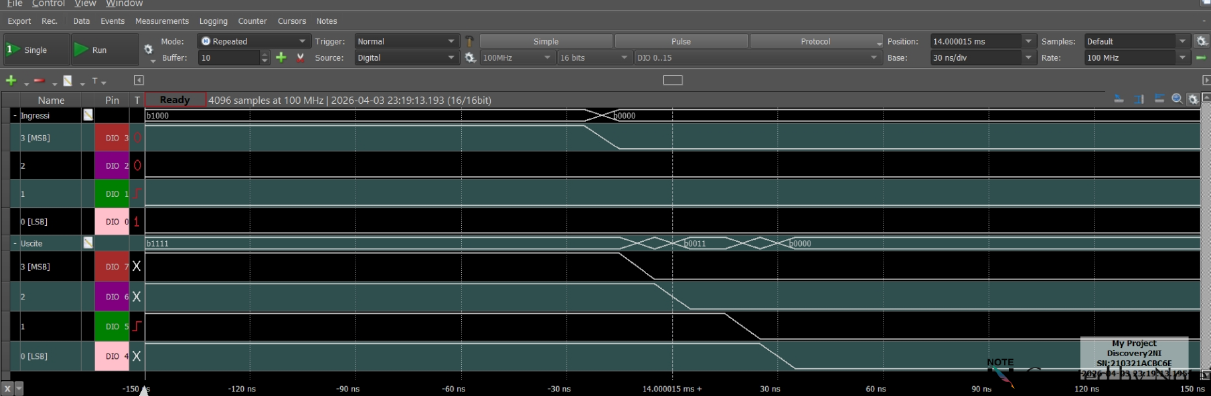
\includegraphics[width=1\linewidth]{1.png}
\end{center}

\noindent Le uscite (gruppo \emph{Uscite}) mostrano le transizioni disallineate dei singoli
bit: da \texttt{b1111} passando per \texttt{b0011} fino a \texttt{b0000}, con i quattro bit
che commutano in istanti diversi (glitch visibile nella zona a cavallo di $t=14{,}000015\,\text{ms}$).
Il registro sincronizzato elimina questi glitch, aggiornando il display solo sul fronte del clock.

% ======================================================================
\chapter{Registri a scorrimento e contatori}
\textit{(17 aprile 2026)}

% ======================================================================
\section{Registri a scorrimento}

I \textbf{registri a scorrimento} agiscono come \textbf{passatori} fra due stati del circuito:
\[
Q_0 = X \to Q_1 = X,\quad Q_0 = Y \to Q_2 = X,\quad Q_1 = Y,\quad Q_0 = Z \to \cdots
\]

\subsection{Modalità di trasmissione dati}

I registri a scorrimento hanno molteplici utilizzi nella trasmissione dati. \textit{(Nota: non è a scorrimento.)}

\begin{itemize}[leftmargin=1.5em]
    \item \textbf{Seriale $\to$ seriale} = \textbf{SISO}: $\text{in} \to [D_2 \to D_1 \to D_0] \to \text{out}$ \hfill \textit{usato per il delaying}
    \item \textbf{Seriale $\to$ parallelo} = \textbf{SIPO}: $\text{in} \to [D_2 \to D_1 \to D_0] \to \text{out}$ \hfill \textit{usato per il filling}
    \item \textbf{Parallelo $\to$ seriale} = \textbf{PISO}: $\text{in} \to [D_2, D_1, D_0] \to \text{out}$ \hfill \textit{usato per il drawing}
    \item \textbf{Parallelo $\to$ parallelo} = \textbf{PIPO}: $\text{in} \to [D_2, D_1, D_0] \to \text{out}$ \hfill \textit{usato per lo storing}
\end{itemize}

I tempi di flip-flop sono sufficientemente brevi, rispettati anche dalla frequenza del clock.

\subsection{Temporizzazione e vincoli}

\defbox{
$T_P > T_H$, \quad $T_S + T_P < T_{CLK}$

\begin{itemize}[leftmargin=1.3em]
  \item $T_{setup}$ e $T_{hold}$: tempi caratteristici del flip-flop rispetto al fronte di clock.
  \item $I_N = D_{SR}$: dato seriale in ingresso.
  \item $Q_0 = D_1$: il primo flip-flop segue l'ingresso.
\end{itemize}
}

\noindent Nei registri sono presenti alcuni controlli:
\begin{itemize}[leftmargin=1.5em]
    \item \textbf{clock} = sincronizza lo shift;
    \item \textbf{reset/clear} = azzera tutto;
    \item \textbf{set} = una segnale;
    \item \textbf{enable} = abilita lo shift.
\end{itemize}

\noindent Si distinguono due tipi di registro:
\begin{itemize}[leftmargin=1.5em]
    \item \textbf{Registri normali (PIPO)}: conservano i dati;
    \item \textbf{Registri a scorrimento}: conservano e spostano i dati.
\end{itemize}

\subsection{Schemi dei registri a scorrimento (SISO, SIPO, PISO)}

Di seguito sono riportati gli schemi a blocchi semplificati per le tre configurazioni più
comuni (ogni blocco è un FF-D con uscite $Q_0$, $\overline{Q_0}$, ingresso $D$ e clock $R$/$CLK$).

\begin{fitcenter}
\begin{circuitikz}[scale=0.75, every node/.style={scale=0.75}]

% -------- PIPO --------
% 2 FF-D in cascata (rappresentativo)
\foreach \i/\xi in {0/0, 1/2.2}{
  \draw (\xi,0) rectangle (\xi+1.8, 2.2);
  \node[font=\scriptsize] at (\xi+0.9, 1.8) {${}^S$};
  \node[font=\scriptsize] at (\xi+0.4, 1.2) {$D_{\i}$};
  \node[font=\scriptsize] at (\xi+0.4, 0.7) {$Q_{\i}$};
  \node[font=\scriptsize] at (\xi+0.4, 0.3) {$\overline{Q_{\i}}$};
  \node[font=\scriptsize] at (\xi+1.4, 0.7) {$R$};
}
\draw[-latex] (-0.8, 1.2) -- (0, 1.2) node[midway,above,font=\tiny]{$D_0$};
\draw[-latex] (1.8, 0.7) -- (2.2, 0.7);
\draw[-latex] (4.0, 0.7) -- (4.6, 0.7) node[right,font=\tiny]{out};
\draw[-latex] (0.9,-0.3) -- (0.9,0) node[right,font=\tiny]{};
\draw (0.9,-0.3) -- (3.1,-0.3);
\draw[-latex] (3.1,-0.3) -- (3.1,0);
\draw (0.9,-0.3) -- (-0.4,-0.3) node[left,font=\tiny]{CLK};
\node[font=\small\bfseries] at (2.0,-0.9) {PIPO};

% -------- SISO --------
\begin{scope}[xshift=6.0cm]
\foreach \i/\xi in {0/0, 1/2.2}{
  \draw (\xi,0) rectangle (\xi+1.8, 2.2);
  \node[font=\scriptsize] at (\xi+0.9, 1.8) {${}^S$};
  \node[font=\scriptsize] at (\xi+0.4, 1.2) {$D_{\i}$};
  \node[font=\scriptsize] at (\xi+0.4, 0.7) {$Q_{\i}$};
  \node[font=\scriptsize] at (\xi+0.4, 0.3) {$\overline{Q_{\i}}$};
  \node[font=\scriptsize] at (\xi+1.4, 0.7) {$R$};
}
\draw[-latex] (-0.8,1.2) -- (0,1.2) node[midway,above,font=\tiny]{in};
\draw[-latex] (1.8,0.7) -- (2.2,1.2);
\draw[-latex] (4.0,0.7) -- (4.6,0.7) node[right,font=\tiny]{out};
\draw (0.9,-0.3) -- (-0.4,-0.3) node[left,font=\tiny]{CLK};
\draw (0.9,-0.3) -- (3.1,-0.3);
\draw[-latex] (0.9,-0.3) -- (0.9,0);
\draw[-latex] (3.1,-0.3) -- (3.1,0);
\node[font=\small\bfseries] at (2.0,-0.9) {SISO};
\end{scope}

% -------- SIPO --------
\begin{scope}[xshift=12.0cm]
\foreach \i/\xi in {0/0, 1/2.2}{
  \draw (\xi,0) rectangle (\xi+1.8, 2.2);
  \node[font=\scriptsize] at (\xi+0.9, 1.8) {${}^S$};
  \node[font=\scriptsize] at (\xi+0.4, 1.2) {$D_{\i}$};
  \node[font=\scriptsize] at (\xi+0.4, 0.7) {$Q_{\i}$};
  \node[font=\scriptsize] at (\xi+0.4, 0.3) {$\overline{Q_{\i}}$};
  \node[font=\scriptsize] at (\xi+1.4, 0.7) {$R$};
}
\draw[-latex] (-0.8,1.2) -- (0,1.2) node[midway,above,font=\tiny]{in};
\draw[-latex] (1.8,0.7) -- (2.2,1.2);
% uscite parallelo
\draw[-latex] (0.9,2.2) -- (0.9,2.7) node[above,font=\tiny]{$Q_0$};
\draw[-latex] (3.1,2.2) -- (3.1,2.7) node[above,font=\tiny]{$Q_1$};
\draw (0.9,-0.3) -- (-0.4,-0.3) node[left,font=\tiny]{CLK};
\draw (0.9,-0.3) -- (3.1,-0.3);
\draw[-latex] (0.9,-0.3) -- (0.9,0);
\draw[-latex] (3.1,-0.3) -- (3.1,0);
\node[font=\small\bfseries] at (2.0,-0.9) {SIPO};
\end{scope}

% -------- PISO --------
\begin{scope}[xshift=18.0cm]
\foreach \i/\xi in {0/0, 1/2.2}{
  \draw (\xi,0) rectangle (\xi+1.8, 2.2);
  \node[font=\scriptsize] at (\xi+0.9, 1.8) {${}^S$};
  \node[font=\scriptsize] at (\xi+0.4, 1.2) {$D_{\i}$};
  \node[font=\scriptsize] at (\xi+0.4, 0.7) {$Q_{\i}$};
  \node[font=\scriptsize] at (\xi+0.4, 0.3) {$\overline{Q_{\i}}$};
  \node[font=\scriptsize] at (\xi+1.4, 0.7) {$R$};
}
% ingressi parallelo
\draw[-latex] (0.9,2.7) -- (0.9,2.2) node[above=0.5cm,font=\tiny]{$D_0$};
\draw[-latex] (3.1,2.7) -- (3.1,2.2) node[above=0.5cm,font=\tiny]{$D_1$};
\draw[-latex] (4.0,0.7) -- (4.6,0.7) node[right,font=\tiny]{out};
\draw (0.9,-0.3) -- (-0.4,-0.3) node[left,font=\tiny]{CLK};
\draw (0.9,-0.3) -- (3.1,-0.3);
\draw[-latex] (0.9,-0.3) -- (0.9,0);
\draw[-latex] (3.1,-0.3) -- (3.1,0);
% sel
\draw[-latex] (2.2,1.8) -- (2.2,2.2) node[above,font=\tiny]{sel};
\node[font=\small\bfseries] at (2.0,-0.9) {PISO};
\end{scope}

\end{circuitikz}
\end{fitcenter}

% ======================================================================
\section{Contatori}
\textit{(17 aprile 2026)}

\defbox{
\textbf{Contatore} = circuito che esegue le transizioni da uno stato al successivo, rappresentando in binario numeri contigui.
}

\begin{itemize}[leftmargin=1.5em]
    \item $Q_0$ cambia ogni periodo (del clock).
    \item $Q_1$ cambia ogni 2 periodi (quando $Q_0$ ha fronte di discesa).
    \item $Q_{i+1}$ cambia ogni $2^{i+1}$ periodi (quando $Q_i$ ha fronte di discesa).
\end{itemize}

\begin{center}
\begin{tikzpicture}[scale=0.85, every node/.style={scale=0.85}]
\draw[-latex] (0,0) -- (8.0,0) node[right]{$t$};
% CLK
\draw[thick] (0,1.2) -- (0.5,1.2) -- (0.5,1.8) -- (1.0,1.8) -- (1.0,1.2) -- (1.5,1.2) -- (1.5,1.8) -- (2.0,1.8) -- (2.0,1.2) -- (2.5,1.2) -- (2.5,1.8) -- (3.0,1.8) -- (3.0,1.2) -- (3.5,1.2) -- (3.5,1.8) -- (4.0,1.8) -- (4.0,1.2) -- (7.5,1.2);
\node[right, font=\small] at (7.5,1.5) {CLK};
% Q0
\draw[thick,blue] (0,0.5) -- (1.0,0.5) -- (1.0,0.9) -- (2.0,0.9) -- (2.0,0.5) -- (3.0,0.5) -- (3.0,0.9) -- (4.0,0.9) -- (4.0,0.5) -- (7.5,0.5);
\node[right, font=\small] at (7.5,0.7) {$Q_0$};
% Q1
\draw[thick,red] (0,-0.3) -- (2.0,-0.3) -- (2.0,0.1) -- (4.0,0.1) -- (4.0,-0.3) -- (7.5,-0.3);
\node[right, font=\small] at (7.5,-0.1) {$Q_1$};
\end{tikzpicture}
\end{center}

\subsection{Contatore asincrono (ripple counter)}

Non tutte le parti del circuito sono guidate dallo stesso clock: \textbf{il contatore è asincrono}. Il clock di ciascun blocco è legato all'uscita del precedente.

Il tempo di propagazione del bit più significativo è $T_n = n\,T_P$.

Deve valere $T_{CLK} > T_n$ per avere un tempo in cui il segnale è stabile.

\begin{center}
\begin{circuitikz}[scale=0.82, every node/.style={scale=0.82}]
% 4 JK FF in cascata (asincrono)
\foreach \i/\xi in {0/0, 1/2.8, 2/5.6, 3/8.4}{
  \draw (\xi,0) rectangle (\xi+2.2, 2.0);
  \node[font=\scriptsize] at (\xi+0.55,1.5) {$K_{\i}$};
  \node[font=\scriptsize] at (\xi+0.55,1.0) {$J_{\i}$};
  \node[font=\scriptsize] at (\xi+1.7,1.0) {$Q_{\i}$};
  \node[font=\scriptsize] at (\xi+1.7,0.4) {$\overline{Q_{\i}}$};
  % J e K collegati a 1
  \draw (\xi+0.2,1.5) -- ++(-0.2,0) coordinate (K\i);
  \draw (\xi+0.2,1.0) -- ++(-0.2,0) coordinate (J\i);
}
% CLK al primo
\draw[-latex] (-1.0,1.0) -- (0,1.0) node[midway,above,font=\scriptsize]{CLK};
\node[font=\scriptsize] at (-0.7,1.8) {$1$};
\draw (-0.5,1.5) -- (0,1.5);
\draw (-0.5,1.0) -- (-0.5,1.5);
% CLK dei successivi collegato a Qi del precedente
\draw[-latex] (2.2,0.4) -- (2.8,0.4) node[midway,below,font=\scriptsize]{};
\draw[-latex] (5.0,0.4) -- (5.6,0.4);
\draw[-latex] (7.8,0.4) -- (8.4,0.4);
% uscite
\draw[-latex] (10.6,1.0) -- (11.2,1.0) node[right,font=\scriptsize]{$Q_3$};
\node[below=0.5cm, font=\small\bfseries, color=noteblue] at (5.3,-0.3) {CONTATORE ASINCRONO};
\end{circuitikz}
\end{center}

\subsection{Contatore sincrono}

Tutte le parti sono guidate dallo stesso clock: ogni uscita dei blocchi è collegata all'uscita del blocco precedente con una porta AND, che fa cambiare stato al successivo \emph{solo se tutte le uscite prima sono sature} (cioè tutte a $1$).

\begin{center}
\begin{circuitikz}[scale=0.82, every node/.style={scale=0.82}]
% 4 JK FF in parallelo sul CLK, con AND in cascata
\foreach \i/\xi in {0/0, 1/3.2, 2/6.4, 3/9.6}{
  \draw (\xi,0) rectangle (\xi+2.4, 2.2);
  \node[font=\scriptsize] at (\xi+0.6,1.7) {$K_{\i}$};
  \node[font=\scriptsize] at (\xi+0.6,1.1) {$J_{\i}$};
  \node[font=\scriptsize] at (\xi+1.85,1.1) {$Q_{\i}$};
  \node[font=\scriptsize] at (\xi+1.85,0.5) {$\overline{Q_{\i}}$};
}
% 1 su J0 e K0
\node[font=\scriptsize] at (-0.4,2.2) {$1$};
\draw[-latex] (-0.3,2.0) -- (0,2.0) -- (0,1.7);
\draw[-latex] (-0.3,2.0) -- (-0.3,1.1) -- (0,1.1);
% CLK comune
\draw[-latex] (-1.2,0.0) -- (-1.2,-0.5) -- (12.0,-0.5);
\foreach \xi in {1.2, 4.4, 7.6, 10.8}{
  \draw[-latex] (\xi,-0.5) -- (\xi,0);
}
\node[left,font=\scriptsize] at (-1.2,0) {CLK};
% AND gates tra i FF (simplified: line from Q_i to J_{i+1}/K_{i+1})
\draw[-latex] (2.4,1.1) -- (3.2,1.1);
\draw[-latex] (2.4,1.7) -- (3.2,1.7);
\draw[-latex] (5.6,1.1) -- (6.4,1.1);
\draw[-latex] (5.6,1.7) -- (6.4,1.7);
\draw[-latex] (8.8,1.1) -- (9.6,1.1);
\draw[-latex] (8.8,1.7) -- (9.6,1.7);
\draw[-latex] (12.0,1.1) -- (12.6,1.1) node[right,font=\scriptsize]{$Q_3$};

\node[below=0.5cm, font=\small\bfseries, color=noteblue] at (6.0,-0.9) {CONTATORE SINCRONO};
\end{circuitikz}
\end{center}

\subsection{Azzeramento dopo un certo conteggio}

Si vuole che a un certo conteggio il contatore ritorni tutto al livello basso (\textbf{azzeramento}): si implementa usando una porta AND; l'ultimo conto dura $T(\text{JK-FF}) + T_P(\text{AND})$.

\medskip
\noindent\textbf{Esempio}: azzeramento dopo il numero 5 (3 bit).

Quando $Q_3 Q_2 Q_1 Q_0 = 0101$ si attiva il clear $\to Q = 0000$ e si ritorna a contare da capo. In questo modo l'ultimo numero ($5$, $= 0101$) dura un tempo pari a $T_f(\text{JK-FF}) + T_P(\text{AND})$.

\begin{center}
\begin{circuitikz}[scale=0.82, every node/.style={scale=0.82}]
% 4 JK FF con RESET asincrono
\foreach \i/\xi in {0/0, 1/2.8, 2/5.6, 3/8.4}{
  \draw (\xi,0) rectangle (\xi+2.2, 2.0);
  \node[font=\scriptsize] at (\xi+0.55,1.5) {$K_{\i}$};
  \node[font=\scriptsize] at (\xi+0.55,1.0) {$J_{\i}$};
  \node[font=\scriptsize] at (\xi+1.7,1.0) {$Q_{\i}$};
  \node[font=\scriptsize] at (\xi+1.7,0.4) {$\overline{Q_{\i}}$};
}
% CLK
\draw[-latex] (-1.0,0.7) -- (0,0.7) node[midway,above,font=\scriptsize]{CLK};
% carry da Qi a CLK_{i+1}
\draw[-latex] (2.2,0.4) -- (2.8,0.4);
\draw[-latex] (5.0,0.4) -- (5.6,0.4);
\draw[-latex] (7.8,0.4) -- (8.4,0.4);
% AND gate per detect di 0101 -> RESET
\node[and port, scale=0.7] (AND) at (6.5,-1.2) {};
\draw (2.2,1.0) -- (2.5,1.0) |- (AND.in 1);
\draw (8.4+1.0,1.0) -- (9.8,1.0) |- (AND.in 2);
\draw (AND.out) -- ++(0.5,0) node[right,font=\scriptsize]{RESET ASINCRONO DI TUTTI i FF};
\node[font=\scriptsize] at (5.0,-1.8) {};
\end{circuitikz}
\end{center}

\subsection{Ripple Carry Output}

Il contatore binario sincrono oltre ai 4 bit di uscita ha anche un \textbf{Ripple Carry Output} (RCO): uscita di una porta NOR con 5 ingressi (i 4 $\overline{Q_i}$ e l'\emph{enable}).

\[
\text{RCO} = 1 \quad \text{(per un periodo } T_{CLK}\text{) quando il conteggio è terminato.}
\]

Segnala, cioè, che il contatore ha raggiunto il valore massimo ed è pronto per ricominciare
(utilizzabile per pilotare il contatore del \emph{digit} successivo in una catena).

\begin{center}
\begin{tikzpicture}[scale=0.85, every node/.style={scale=0.85}]
% Schema a blocchi del SN74LS163A (stilizzato)
\draw (0,0) rectangle (4.5,5.5);
\node[font=\small\bfseries] at (2.25,5.1) {SN74LS163A};
% Ingressi sincroni
\foreach \y/\lab in {4.5/CLK, 4.0/$Q_A$, 3.5/$Q_B$, 3.0/$Q_C$, 2.5/$Q_D$}{
  \draw[-latex] (-1.0,\y) -- (0,\y) node[midway,above,font=\scriptsize]{\lab};
}
% Ingressi DATA
\foreach \y/\lab in {2.0/DATA A, 1.5/DATA B, 1.0/DATA C, 0.5/DATA D}{
  \draw[-latex] (-1.2,\y) -- (0,\y) node[midway,above,font=\tiny]{\lab};
}
% Uscite
\foreach \y/\lab in {4.5/$Q_A$, 3.5/$Q_B$, 2.5/$Q_C$, 1.5/$Q_D$}{
  \draw[-latex] (4.5,\y) -- (5.5,\y) node[right,font=\scriptsize]{\lab};
}
\draw[-latex] (4.5,0.7) -- (5.5,0.7) node[right,font=\scriptsize]{RCO};
% Enable e Load
\draw[-latex] (-1.0,-0.3) -- (2.25,-0.3) -- (2.25,0) node[right,font=\tiny]{ENABLE/LOAD};
\node[font=\tiny, align=center] at (2.25,0.5) {CLOCK\\DATA INPUT};
\end{tikzpicture}
\end{center}

% ======================================================================
\chapter{Conteggio, divisori di frequenza e PRFG}
\textit{(20 aprile 2026)}

% ======================================================================
\section{Contatori a 8 bit: cascata di due SN74LS163}

Due contatori sincroni a 4 bit si collegano in \textbf{cascata} tramite il segnale RCO:
il bit più significativo (\emph{MSB}, gestito dal secondo 163) viene incrementato quando
il contatore meno significativo (\emph{LSB}) raggiunge il valore 15 e porta $\text{RCO}=1$.
Il segnale RCO del primo modulo funge da \emph{enable di conteggio} per il secondo.

\begin{center}
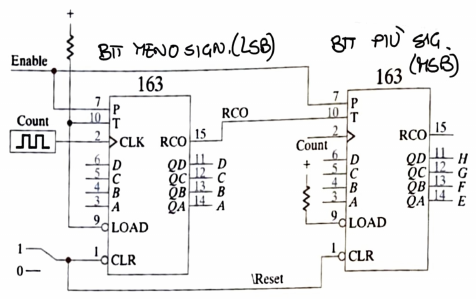
\includegraphics[width=0.85\linewidth]{img_cascata.png}
\end{center}

\noindent Due contatori sincroni a 4 bit si collegano a cascata con il RCO che funge da
\emph{enable di conteggio}: il contatore MSB avanza di un'unità ogni volta che il LSB
arriva a 15 ($\text{RCO}=1$). In questo modo si ottiene un contatore a 8 bit capace di
rappresentare i valori da 0 a 255 ($2^8-1$). Le uscite del secondo modulo ($H$, $G$, $F$,
$E$) sono i bit più significativi dell'intero conteggio; il segnale $\overline{\text{Reset}}$
asincrono è comune ad entrambi i moduli.

% ======================================================================
\section{Divisori di frequenza per un numero $n$}
\textit{(20 aprile 2026)}

\defbox{
\textbf{Divisore di frequenza} = circuito sequenziale che prende in ingresso il segnale
di clock e ne riduce la frequenza di un fattore $n$:
\[
f_{\text{out}} = \frac{f_{\text{CLK}}}{n} \qquad T_{\text{out}} = n\,T_{\text{CLK}}
\]
}

\noindent Si realizzano con il contatore SN74LS163 sfruttando il segnale RCO o il LOAD.
Esistono due varianti principali.

\subsection{Divisore con CLEAR sincrono}

Il circuito conta fino a $\text{DCBA}=1101$ (13); dopodich\'e il CLEAR \`e 1 e ricomincia
da capo.

\begin{center}
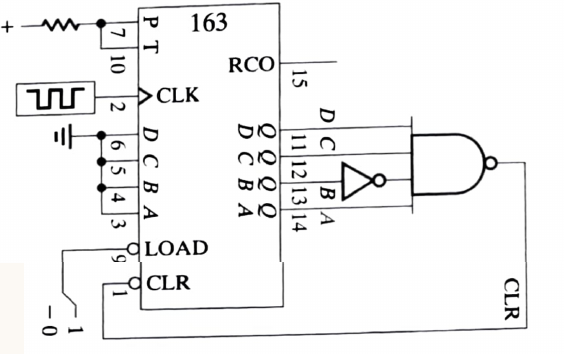
\includegraphics[width=0.52\linewidth]{img_clear.png}
\end{center}

\begin{itemize}[leftmargin=1.5em]
    \item $A$ (LSB) ha $T_A = 2\,T_{\text{CLK}}$.
    \item $D$ (MSB) ha $T_D = 16\,T_{\text{CLK}}$.
    \item Il numero 13 è l'ultimo contato, con $f = f_{\text{CLK}}/14$.
    \item Senza il clear sincrono l'ultimo stato (13) dura poco, non è esattamente un fronte.
\end{itemize}

\noindent\textit{Funzionamento}: le uscite $Q_D Q_C Q_B Q_A$ vengono decodificate da una
porta AND (con buffer invertente sul segnale $C$ per selezionare il pattern $1101$); quando
l'AND vale 1, il segnale CLR si attiva e azzera il contatore al colpo di clock successivo.
L'uscita CLR torna quindi a 0 e il ciclo ricomincia.

\subsection{Divisore con SET sincrono (LOAD)}

Il circuito ha il RCO collegato al LOAD (set) in modo che, dopo aver finito di contare,
venga caricato il valore impostato su $\text{DCBA}=0110$ (6).

\begin{center}
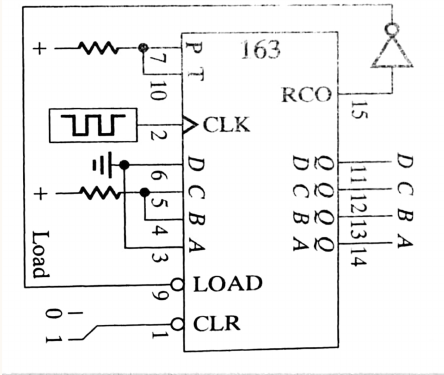
\includegraphics[width=0.52\linewidth]{img_set.png}
\end{center}

\begin{itemize}[leftmargin=1.5em]
    \item RCO ha una frequenza di $4/\text{ciclo}$ $T_{\text{CLK}}$ ($1/10$).
    \item In generale: $T_s = (2^n - n_{\text{load}})\,T_{\text{CLK}}$.
\end{itemize}

\noindent\textit{Funzionamento}: quando il contatore raggiunge 15 e $\text{RCO}=1$, al
colpo di clock successivo il LOAD forza il caricamento del valore preset ($\text{DCBA}=0110$
in questo esempio); il contatore riparte da 6 anziché da 0, ottenendo un ciclo di lunghezza
$16-6=10$, cioè $f_{\text{out}} = f_{\text{CLK}}/10$. Il LED collegato all'RCO si
accende una volta per ciclo.

% ======================================================================
\section{Contatore ad anello}

Si pone in ingresso $Q=0001$ e si applica il clock per vedere come evolve:

\[
0001 \to 0010 \to 0100 \to 1000
\]

I FF copiano il valore in entrata: contatore con solo \textbf{4 valori}.

\begin{center}
\begin{circuitikz}[scale=0.82, every node/.style={scale=0.82}]
% 4 FF-D in anello
\foreach \i/\xi in {0/0, 1/2.6, 2/5.2, 3/7.8}{
  \draw (\xi,0) rectangle (\xi+2.0,1.8);
  \node[font=\scriptsize] at (\xi+0.5,1.3) {$D_{\i}$};
  \node[font=\scriptsize] at (\xi+1.5,1.3) {$Q_{\i}$};
  \node[font=\scriptsize] at (\xi+1.5,0.5) {$\overline{Q_{\i}}$};
}
% collegamento Q_{i} -> D_{i+1}
\draw[-latex] (2.0,1.3) -- (2.6,1.3);
\draw[-latex] (4.6,1.3) -- (5.2,1.3);
\draw[-latex] (7.2,1.3) -- (7.8,1.3);
% feedback anello: Q3 -> D0
\draw (9.8,1.3) -- (9.8,2.2) -- (-0.4,2.2) -- (-0.4,1.3) -- (0,1.3);
% CLK comune
\draw[-latex] (-1.2,-0.3) -- (-1.2,-0.6) -- (9.6,-0.6);
\foreach \xi in {1.0,3.6,6.2,8.8}{
  \draw[-latex] (\xi,-0.6) -- (\xi,0);
}
\node[left,font=\scriptsize] at (-1.2,0) {CLK};
\end{circuitikz}
\end{center}

\section{Contatore ad anello \emph{twisted} (Johnson counter)}

Si pone in ingresso $Q=0000$ e si applica il clock; si nota che $\overline{Q_3}$ è
collegato a $D_0$ (feedback invertito):

\[
0000 \to 0001 \to 0011 \to 0111 \to 1111 \to 1110 \to 1100 \to 1000 \to 0000
\]

I FF copiano il valore in entrata: contatore con \textbf{8 valori} (con 4 FF).

\begin{center}
\begin{circuitikz}[scale=0.82, every node/.style={scale=0.82}]
% 4 FF-D in anello twisted
\foreach \i/\xi in {0/0, 1/2.6, 2/5.2, 3/7.8}{
  \draw (\xi,0) rectangle (\xi+2.0,1.8);
  \node[font=\scriptsize] at (\xi+0.5,1.3) {$D_{\i}$};
  \node[font=\scriptsize] at (\xi+1.5,1.3) {$Q_{\i}$};
  \node[font=\scriptsize] at (\xi+1.5,0.5) {$\overline{Q_{\i}}$};
}
% collegamento Q_{i} -> D_{i+1}
\draw[-latex] (2.0,1.3) -- (2.6,1.3);
\draw[-latex] (4.6,1.3) -- (5.2,1.3);
\draw[-latex] (7.2,1.3) -- (7.8,1.3);
% feedback twisted: Qbar_3 -> D0
\draw (9.8,0.5) -- (9.8,-0.9) -- (-0.4,-0.9) -- (-0.4,1.3) -- (0,1.3);
\node[font=\scriptsize] at (10.3,0.5) {$\overline{Q_3}$};
% CLK comune
\draw[-latex] (-1.2,0.9) -- (0,0.9);
\foreach \xi in {2.6,5.2,7.8}{
  \draw[-latex] (\xi-0.3,0.9) -- (\xi,0.9);
}
\node[left,font=\scriptsize] at (-1.2,0.9) {CLK};
\end{circuitikz}
\end{center}

\defbox{
Rispetto al contatore ad anello normale, il Johnson counter ha \textbf{2N stati} per N
flip-flop utilizzati per realizzarlo.
}

% ======================================================================
\section{Generatori di frequenza pseudo casuali (PRFG)}

\defbox{
\textbf{PRFG} (\emph{Pseudo-Random Frequency Generator}) = applicazione dei registri a
scorrimento che ha trovato grande applicazione nella generazione di sequenze di bit pseudo
casuali. Il registro ha grandezza fissa; questo comporta lo ``pseudo''.\\[0.3em]
Un registro largo $K$ FF genera una sequenza ripetuta al massimo dopo $2^K-1$ eventi.
}

\noindent Nei generatori pseudo casuali \textbf{lineari} si usa lo XOR (o XNOR) per
costruire il circuito: le porte equivalenti alla somma binaria.

\defbox{
\textbf{LPRG} = \emph{Linear Pseudo Random Generator}
}

\begin{center}
\begin{circuitikz}[scale=0.82, every node/.style={scale=0.82}]
% 4 FF-D con feedback XOR (LFSR)
\foreach \i/\xi in {0/0, 1/2.6, 2/5.2, 3/7.8}{
  \draw (\xi,0) rectangle (\xi+2.0,1.8);
  \node[font=\scriptsize] at (\xi+0.5,1.3) {$D_{\i}$};
  \node[font=\scriptsize] at (\xi+1.5,1.3) {$Q_{\i}$};
  \node[font=\scriptsize] at (\xi+1.5,0.5) {$\overline{Q_{\i}}$};
}
% shift: Q_{i} -> D_{i+1}
\draw[-latex] (2.0,1.3) -- (2.6,1.3);
\draw[-latex] (4.6,1.3) -- (5.2,1.3);
\draw[-latex] (7.2,1.3) -- (7.8,1.3);
% XOR gate per feedback
\node[xor port, scale=0.7] (XF) at (1.3, 3.0) {};
% Q3 -> XOR in1 (feedback)
\draw (9.8,1.3) -- (9.8,3.0) -- (XF.in 1);
% Q0 (o altro tap) -> XOR in2
\draw (2.0,1.3) -- (2.0,2.4) -- (XF.in 2);
% XOR out -> D0
\draw[-latex] (XF.out) -- (0,3.0) -- (0,1.8);
% CLK comune
\draw[-latex] (-1.2,-0.4) -- (-1.2,-0.7) -- (9.6,-0.7);
\foreach \xi in {1.0,3.6,6.2,8.8}{
  \draw[-latex] (\xi,-0.7) -- (\xi,0);
}
\node[left,font=\scriptsize] at (-1.2,0) {CLK};
\end{circuitikz}
\end{center}

\noindent La tabella degli stati del LPRG a 3 FF (FF0, FF1, FF2), con feedback XOR tra
FF2 e FF1, mostra la sequenza pseudo casuale di lunghezza $2^3-1=7$:

\begin{center}
\begin{tabular}{c|ccc}
\toprule
Clock & FF0 & FF1 & FF2 \\
\midrule
0 & 1 & 1 & 1 \\
1 & 0 & 1 & 1 \\
2 & 1 & 0 & 1 \\
3 & 1 & 1 & 0 \\
4 & 0 & 1 & 1 \\
5 & 1 & 0 & 1 \\
6 & 0 & 0 & 1 \\
7 & 1 & 0 & 0 \\
8 & 1 & 1 & 0 \\
9 & 0 & 1 & 1 \\
10 & 0 & 0 & 1 \\
11 & 1 & 0 & 0 \\
12 & 1 & 1 & 0 \\
13 & 1 & 1 & 1 \\
\bottomrule
\end{tabular}
\end{center}

% ======================================================================
\chapter{Macchine a stati finiti (FSM)}
\textit{(24 aprile 2026)}

\defbox{
\textbf{FSM} (\emph{Finite State Machine}) = architettura in cui gli stati presenti
determinano quelli futuri.
}

\defbox{
\textbf{Diagramma di stato} = mappa per rappresentare il comportamento di un sistema
sequenziale (possibili stati e legami).\\[0.3em]
Gli stati sono legati fra loro da precise transizioni. Gli stati sono definiti da
condizioni \textbf{INTERNE} (presenti nel sistema) e/o da condizioni \textbf{ESTERNE}
(segnali in ingresso dall'esterno).
}

\noindent Ogni circuito digitale è una FSM.

% ======================================================================
% Continuazione Capitolo 8: Macchine a stati finiti (FSM)
% (24 aprile 2026)
% ======================================================================

\section{Tipi di architettura FSM: Moore e Mealy}

Esistono due tipi principali di architettura per le FSM:

\begin{itemize}[leftmargin=1.5em]
    \item \textbf{Architettura di Moore}
    \item \textbf{Architettura di Mealy}
\end{itemize}

\subsection{Architettura di Moore}

\begin{center}
\begin{tikzpicture}[scale=0.85, every node/.style={scale=0.85},
  box/.style={draw, minimum width=2.0cm, minimum height=1.0cm, align=center, font=\small}]

\node[box] (lcf) at (0,0)    {logica\\combinatoria\\stato futuro};
\node[box] (reg) at (3.6,0)  {registro\\di\\memoria};
\node[box] (lcu) at (7.2,0)  {logica\\combinatoria\\uscite};

% Frecce principali
\draw[-latex] (-1.8,0) -- (lcf.west) node[midway,above,font=\scriptsize]{ingressi};
\draw[-latex] (lcf.east) -- (reg.west) node[midway,above,font=\scriptsize]{futuro};
\draw[-latex] (reg.east) -- (lcu.west) node[midway,above,font=\scriptsize]{presente};
\draw[-latex] (lcu.east) -- ++(1.4,0) node[right,font=\scriptsize]{uscite};

% CLK al registro
\draw[-latex] (3.6,-1.2) -- (reg.south) node[below=1.0cm,font=\scriptsize]{CLK};

% Feedback dallo stato presente alla logica combinatoria stato futuro
\draw[-latex] (3.6,0.5) -- (3.6,1.4) -- (-0.2,1.4) -- (-0.2,0.5);

% bus (freccia dal basso dell'uscita)
\draw[-latex] (8.0,-0.5) -- (8.0,-1.2) node[below,font=\scriptsize]{bus};

\end{tikzpicture}
\end{center}

\begin{itemize}[leftmargin=1.5em]
    \item Uno stato è univocamente conseguenza dello stato precedente.
    \item Gli ingressi esterni non sempre sono presenti.
\end{itemize}

% ======================================================================
\section{Dal diagramma di stato al circuito}
\textit{(24 aprile 2026)}

\noindent Il diagramma di stato è composto da \textbf{stati} (cerchi etichettati con il
valore di uscita) collegati da \textbf{transizioni} (frecce etichettate con il valore
dell'ingresso/condizione):

\begin{center}
\begin{tikzpicture}[scale=0.9, every node/.style={scale=0.9},
  state/.style={draw, circle, minimum size=1.0cm, font=\small, align=center}]

\node[state] (s0) at (0,0)    {$S_0$ \\ {\tiny 00}};
\node[state] (s1) at (2.4,-1.2)  {$S_1$ \\ {\tiny 011}};
\node[state] (s2) at (-2.4,-1.2) {$S_2$ \\ {\tiny 101}};

\draw[-latex] (s0) -- (s1);
\draw[-latex] (s1) -- (s2);
\draw[-latex] (s2) -- (s0);

\node[above right, font=\scriptsize] at (s0.north east) {stato};
\node[below, font=\scriptsize] at (s1.south) {valore di uscita};
\node[left,  font=\scriptsize] at (-1.5,-1.8) {transizione};
\node[above, font=\scriptsize, color=noteteal] at (0.6,-0.4) {diagramma di stato};

\end{tikzpicture}
\end{center}

\noindent La procedura per passare dal diagramma di stato al circuito è la seguente:

\begin{enumerate}[leftmargin=1.5em]
    \item \textbf{Dato il numero di stati} (3) definisco il numero di bit che mi serve a
          rappresentarli: $\lceil\log_2 3\rceil = 2\;\Rightarrow\;$ 2 bit.
    \item \textbf{Associo a ogni stato una rappresentazione in bit}:
          $S_0=[00]$, $S_1=[01]$, $S_2=[10]$, $S_3=[X]$ \emph{(don't care)}.
    \item \textbf{Per ogni bit uso un FF}: $S_i = Q_i Q_0^i$.
    \item \textbf{Scrivo la tabella di verità}: associo a ogni stato presente uno stato
          futuro.

\begin{center}
\begin{tabular}{cc|cc}
\toprule
$Q_1$ & $Q_0$ & $Q_1^+$ & $Q_0^+$\\
\midrule
0 & 0 & 0 & 1\\
0 & 1 & 1 & 0\\
1 & 0 & 0 & 0\\
1 & 1 & $\times$ & $\times$\\
\bottomrule
\end{tabular}
\end{center}

    \item \textbf{Scelgo il tipo di FF} (D, JK, T): in questo caso uso DFF,
          poiché $Q^+=D$.
    \item \textbf{Ricavo le funzioni di $D_i = f(Q_i)$}:
          \[
          D_1 = Q_0 \qquad D_0 = \overline{Q_1}\cdot\overline{Q_0}
          \]
    \item \textbf{Disegno il circuito}:

\begin{center}
\begin{circuitikz}[scale=0.85, every node/.style={scale=0.85}]
% Due DFF in cascata
\draw (0,0) rectangle (1.8,2.0);
\node[font=\scriptsize] at (0.5,1.5) {$D_0\,Q_0$};
\node[font=\scriptsize] at (0.5,0.5) {$\overline{Q_0}$};
\draw (2.8,0) rectangle (4.6,2.0);
\node[font=\scriptsize] at (3.3,1.5) {$D_1\,Q_1$};
\node[font=\scriptsize] at (3.3,0.5) {$\overline{Q_1}$};

% D0 <- feedback da Q0 (D0 = Qbar1 * Qbar0, semplificato come segnale)
\draw[-latex] (-1.0,1.5) -- (0,1.5) node[midway,above,font=\tiny]{$D_0$};
% Q0 -> D1
\draw[-latex] (1.8,1.5) -- (2.8,1.5) node[midway,above,font=\tiny]{$Q_0$};
% Uscita Q1
\draw[-latex] (4.6,1.5) -- (5.4,1.5) node[right,font=\tiny]{$Q_1$};

% CLK comune
\draw[-latex] (-1.0,-0.5) -- (0.9,-0.5) -- (0.9,0) node[above,font=\tiny]{};
\draw (0.9,-0.5) -- (3.7,-0.5);
\draw[-latex] (3.7,-0.5) -- (3.7,0);
\node[left,font=\scriptsize] at (-1.0,-0.5) {CLK};
\end{circuitikz}
\end{center}

\end{enumerate}

\defbox{
\begin{itemize}[leftmargin=1.3em,itemsep=2pt]
    \item \textbf{DFF}: $Q^+=D$ \quad più usato, semplice.
    \item \textbf{TFF}: $Q^+=T\oplus Q$ \quad per contatori e sequenze regolari.
    \item \textbf{JKFF}: flessibile, può fare tutto (set, reset, toggle).
\end{itemize}
}

\subsection{Ricavare le funzioni dei segnali di uscita: $O_i = f(Q_i)$}

\begin{center}
\begin{tabular}{cc|cc|ccc}
\toprule
$Q_1$ & $Q_0$ & $D_0$ & $D_1$ & $O_2$ & $O_1$ & $O_0$\\
\midrule
0 & 0 & 1 & 0 & 0 & 1 & 0\\
0 & 1 & 0 & 1 & 0 & 1 & 1\\
1 & 0 & 0 & 0 & 1 & 0 & 1\\
1 & 1 & $\times$ & $\times$ & $\times$ & $\times$ & $\times$\\
\bottomrule
\end{tabular}
\end{center}

\[
O_0 = Q_0 + Q_1 \qquad O_1 = \overline{Q_1} \qquad O_2 = Q_1
\]

\subsection{Stato bloccante e segnale di Enable}

Al punto 9 si verifica quale sia lo stato futuro del caso $Q_1 = Q_0 = 1$: se è uno
\textbf{stato bloccante}, è un problema che dobbiamo risolvere.

\noindent Nel nostro caso, da $Q=11$ si andrà a finire in $D=10$, quindi ricomincerà la
sequenza (non blocca il circuito).

\medskip
\noindent Se volessimo scorrere il ciclo al contrario, possiamo inserire un segnale di
\textbf{Enable}:

\begin{itemize}[leftmargin=1.5em]
    \item $E=1$: si ha $010 \to 011 \to 101$ \quad (dritto).
    \item $E=0$: si ha $101 \to 011 \to 010$ \quad (rovescio).
\end{itemize}

\noindent Cambiamo le entrate $D_i$ ma le uscite restano le stesse:
\[
D_i = f(Q_i, E) \qquad O_i = f(Q_i)
\]

\noindent Possiamo scrivere le funzioni:
\[
D_1 = \overline{E}\cdot\overline{Q_1}\cdot\overline{Q_0} + E\cdot Q_0
\qquad
D_0 = E\cdot\overline{Q_1}\cdot\overline{Q_0} + \overline{E}\cdot Q_1
\]

\begin{center}
\begin{tikzpicture}[scale=0.85, every node/.style={scale=0.85},
  state/.style={draw, circle, minimum size=0.9cm, font=\scriptsize, align=center}]

% Diagramma di stato con Enable
\node[state] (s0) at (0,0)       {$S_0$ \\ {\tiny 00}};
\node[state] (s1) at (2.2,-1.0)  {$S_1$ \\ {\tiny 011}};
\node[state] (s2) at (-2.2,-1.0) {$S_2$ \\ {\tiny 101}};

\draw[-latex,bend left=15] (s0) to (s1);
\draw[-latex,bend left=15] (s1) to (s2);
\draw[-latex,bend left=15] (s2) to (s0);

\end{tikzpicture}
\hspace{1.5cm}
\begin{circuitikz}[scale=0.82, every node/.style={scale=0.82}]
% Schema a blocchi con Enable
\draw (1.5,0) rectangle (3.3,2.2);
\node[font=\scriptsize] at (2.1,1.7) {$D_0\,Q_0$};
\node[font=\scriptsize] at (2.1,0.5) {$\overline{Q_0}$};

\draw (4.2,0) rectangle (6.0,2.2);
\node[font=\scriptsize] at (4.8,1.7) {$D_1\,Q_1$};
\node[font=\scriptsize] at (4.8,0.5) {$\overline{Q_1}$};

% E entra nella logica a sinistra
\draw[-latex] (0.0,1.7) -- (1.5,1.7) node[midway,above,font=\tiny]{$D_0$};
\draw[-latex] (-0.5,2.5) -- (0.8,2.5) -- (0.8,1.7) node[near start,above,font=\tiny]{$E$};

% Q0 -> D1
\draw[-latex] (3.3,1.7) -- (4.2,1.7);
% Uscite
\draw[-latex] (6.0,1.7) -- (6.8,1.7) node[right,font=\tiny]{$Q_1$};

% CLK
\draw[-latex] (0.2,-0.9) -- (2.4,-0.9) -- (2.4,0);
\draw (2.4,-0.9) -- (5.1,-0.9);
\draw[-latex] (5.1,-0.9) -- (5.1,0);
\node[left,font=\scriptsize] at (0.2,-0.9) {CLK};

% Label logiche
\node[below=0.3cm,font=\scriptsize,align=center,color=noteteal] at (0.7,0)
      {logica che mi permette\\di ottenere $D_i=f(Q_i,E)$};
\node[below=0.3cm,font=\scriptsize,align=center,color=noteteal] at (6.5,0)
      {logica che permette\\di ottenere $O_i=f(Q_i)$};
\end{circuitikz}
\end{center}

% ======================================================================
% Seguito Capitolo 8 -- Macchine a stati finiti (FSM)
% Continuazione esempio insegna luminosa + Architettura di Mealy
% (27 aprile 2026)
% ======================================================================

\subsection{Esempio: insegna luminosa (continuazione)}

La sequenza dell'insegna luminosa, con $E=1$, è:
\[
RABA \to RABS \to RSBA \to RABA \to \cdots \quad (E=1)
\]
\[
BA \to BS \to BA \to \cdots \quad (E=0, \text{ RS costante})
\]

\noindent Per aggiungere lo stato ``$RS$ costante'' disabilitato, dobbiamo aggiungere un
4\textdegree{} stato, perché $O_i \leftrightarrow f(Q_i) \not\ni E$.

\begin{center}
\begin{tikzpicture}[scale=0.88, every node/.style={scale=0.88},
  state/.style={draw, circle, minimum size=1.1cm, font=\scriptsize, align=center}]

% Diagramma Moore (sinistra)
\node[state] (s0M) at (0, 2.0) {$S_0$\\{[RB]}};
\node[state] (s1M) at (-1.4, 0) {$S_1$\\{[R]}};
\node[state] (s2M) at (1.4, 0)  {$S_2$\\{[B]}};

\draw[-latex, dashed, bend left=15] (s0M) to node[right,font=\tiny]{R} (s1M);
\draw[-latex, dashed, bend left=15] (s1M) to node[below,font=\tiny]{B} (s2M);
\draw[-latex, dashed, bend left=15] (s2M) to node[right,font=\tiny]{} (s0M);
\draw[-latex] (s0M) to[bend right=30] node[left,font=\tiny]{} (s1M);

\node[font=\small\bfseries] at (0,-1.0) {Moore};

% Diagramma Mealy (destra) con stato S3 disabilitato
\begin{scope}[xshift=5.5cm]
\node[state] (s0) at (0, 2.0) {$S_0$\\{[RB]}};
\node[state] (s1) at (-1.4, 0) {$S_1$\\{[R]}};
\node[state] (s2) at (1.4, 0)  {$S_2$\\{[B]}};
\node[state] (s3) at (1.4,-1.6) {$S_3$\\{[-]}};

\draw[-latex, dashed, bend left=15] (s0) to (s1);
\draw[-latex, dashed, bend left=15] (s1) to (s2);
\draw[-latex, dashed, bend left=15] (s2) to (s0);
% S3 con E=0+1
\draw[-latex] (s3) to[bend left=20] (s2);
\node[right, font=\scriptsize, color=noteteal] at (2.0,-0.8) {$E\!=\!0\!+\!1$};

\node[font=\small\bfseries] at (0,-2.4) {Mealy};
\end{scope}

\end{tikzpicture}
\end{center}

\noindent Possiamo quindi implementare l'architettura di Moore.

% ======================================================================
\section{Architettura di Mealy}
\textit{(27 aprile 2026)}

\begin{center}
\begin{tikzpicture}[scale=0.85, every node/.style={scale=0.85},
  box/.style={draw, minimum width=2.0cm, minimum height=1.0cm, align=center, font=\small}]

\node[box] (lcf) at (0,0)   {logica\\combinatoria\\stato futuro};
\node[box] (reg) at (3.6,0) {registro\\di\\memoria};
\node[box] (lcu) at (7.2,0) {logica\\combinatoria\\uscite};

\draw[-latex] (-2.0,0) -- (lcf.west) node[midway,above,font=\scriptsize]{ingressi};
\draw[-latex] (lcf.east) -- (reg.west) node[midway,above,font=\scriptsize]{futuro};
\draw[-latex] (reg.east) -- (lcu.west) node[midway,above,font=\scriptsize]{presente};
\draw[-latex] (lcu.east) -- ++(1.4,0) node[right,font=\scriptsize]{uscite};

% CLK
\draw[-latex] (3.6,-1.2) -- (reg.south) node[below=1.0cm,font=\scriptsize]{CLK};

% Feedback: stato presente -> logica stato futuro
\draw[-latex] (3.6, 0.5) -- (3.6,1.4) -- (-0.2,1.4) -- (-0.2,0.5);

% Differenza: ingressi vanno anche alla logica uscite (linea tratteggiata)
\draw[-latex, dashed] (-1.4,0) -- (-1.4,-1.0) -- (7.2,-1.0) -- (7.2,-0.5);

\end{tikzpicture}
\end{center}

\noindent La differenza principale fra Moore e Mealy è la dipendenza delle uscite dai
parametri del circuito:
\begin{itemize}[leftmargin=1.5em]
    \item in \textbf{Moore}: $O_i = f(Q_i)$, sincrona al clock.
    \item in \textbf{Mealy}: $O_i = f(Q_i, I_i)$, asincrona.
\end{itemize}

\noindent Il valore delle uscite si associa alle \textbf{transizioni}. Riprendendo l'esempio
dell'insegna luminosa, il diagramma di Mealy è:

\begin{center}
\begin{tikzpicture}[scale=0.9, every node/.style={scale=0.9},
  state/.style={draw, circle, minimum size=1.0cm, font=\scriptsize, align=center}]

\node[state] (s0) at (0,0)    {$S_0$\\{\tiny 00}};
\node[state] (s1) at (-2.0,-1.6) {$S_1$\\{\tiny 01}};
\node[state] (s2) at (2.0,-1.6)  {$S_2$\\{\tiny 10}};

% Transizioni con etichette RB, R, B
\draw[-latex, bend left=10] (s0) to node[left, font=\scriptsize]{$-$} (s1);
\draw[-latex, bend left=10] (s1) to node[below, font=\scriptsize]{B} (s2);
\draw[-latex, bend left=10] (s2) to node[right, font=\scriptsize]{R} (s0);
\draw[-latex] (s0) to[loop above] node[font=\scriptsize]{RB} (s0);

% Ingressi E su transizioni
\node[above left, font=\tiny] at (-0.4, -0.6) {$RB$};

\end{tikzpicture}
\end{center}

\begin{itemize}[leftmargin=1.5em]
    \item $E=1$: l'uscita è legata al passaggio fra 2 stati, non allo stato di per sé.
    \item $E=0$: il fronte di clock è asincrono, perché dipende anche da $E$, che è
          asincrono: se il clock si ferma ma $E$ cambia, allora le uscite cambiano.
\end{itemize}

\noindent Per implementare il circuito dei registri si usano JKFF in modalità
``\textbf{toggle}'' (1) oppure ``\textbf{hold}'' (0): $J=K$ in una sola modalità.

\subsection{Tabella di verità dell'insegna luminosa (Mealy)}

\begin{center}
\begin{tabular}{cc|cc|cc}
\toprule
\multicolumn{2}{c|}{} & \multicolumn{2}{c|}{stato futuro} & \multicolumn{2}{c}{uscite}\\
$Q_1$ & $Q_0$ & $Q_1^+$ & $Q_0^+$ & $R$ & $B$\\
\midrule
\multicolumn{6}{l}{$E=1$}\\
\midrule
0 & 0 & 0 & 1 & 1 & 1\\
0 & 1 & 1 & 0 & 1 & 0\\
1 & 0 & 0 & 0 & 0 & 1\\
1 & 1 & $\times$ & $\times$ & $\times$ & $\times$\\
\midrule
\multicolumn{6}{l}{$E=0$}\\
\midrule
0 & 0 & 0 & 0 & 1 & 0\\
0 & 1 & 0 & 1 & 0 & 1\\
1 & 0 & 0 & 1 & 0 & 1\\% [DA VERIFICARE: riga 1,0 con E=0 — leggibile come Q+=01]
1 & 1 & $\times$ & $\times$ & $\times$ & $\times$\\
\bottomrule
\end{tabular}
\end{center}

\subsection{Tabella JK per l'implementazione}

Usando JKFF con $J=K$ (modalità toggle quando $Q_i \neq Q_i^+$, hold quando $Q_i = Q_i^+$):

\begin{center}
\begin{tabular}{cc|cc|cc}
\toprule
$Q_1$ & $Q_0$ & $Q_1^+$ & $Q_0^+$ & $JK_1$ & $JK_0$\\
\midrule
\multicolumn{6}{l}{$E=1$}\\
\midrule
0 & 0 & 0 & 1 & 0 & 1\\
0 & 1 & 1 & 0 & 1 & 1\\
1 & 0 & 0 & 0 & 1 & 0\\
1 & 1 & $\times$ & $\times$ & $\times$ & $\times$\\
\midrule
\multicolumn{6}{l}{$E=0$}\\
\midrule
0 & 0 & 0 & 0 & 0 & 0\\% hold su entrambi
0 & 1 & 0 & 1 & 0 & 0\\
1 & 0 & 0 & 1 & 1 & 1\\
1 & 1 & $\times$ & $\times$ & $\times$ & $\times$\\
\bottomrule
\end{tabular}
\end{center}

\begin{itemize}[leftmargin=1.5em]
    \item Quando $Q_i = Q_i^+$: fa \textbf{hold} ($JK=0$).
    \item Quando $\overline{Q_i} = Q_i^+$: fa \textbf{toggle} ($JK=1$).
\end{itemize}

\[
Q_1^+ = E\,Q_0 \qquad\qquad Q_0^+ = \overline{Q_0}\,(\overline{E}+\overline{Q_1})
\]

\subsection{Mappe di Karnaugh per $JK_0$ e $JK_1$}

\begin{fitcenter}
\begin{tikzpicture}[scale=0.82, every node/.style={scale=0.82}]

% --- Mappa JK0 ---
\node[font=\small] at (2.0,3.2) {Mappa $JK_0$};
\draw (0,0) grid (4,2);
% header colonne Gray: Q1Q0 = 00, 01, 11, 10
\node[font=\scriptsize] at (0.5,2.35) {00};
\node[font=\scriptsize] at (1.5,2.35) {01};
\node[font=\scriptsize] at (2.5,2.35) {11};
\node[font=\scriptsize] at (3.5,2.35) {10};
\node[font=\scriptsize, anchor=east] at (-0.1,1.5) {0};
\node[font=\scriptsize, anchor=east] at (-0.1,0.5) {1};
\node[font=\scriptsize] at (-0.7,2.35) {$E\backslash Q_1Q_0$};
% Valori: riga E=0: 0,0,X,0; riga E=1: 1,1,X,0
\node at (0.5,1.5) {0}; \node at (1.5,1.5) {0}; \node at (2.5,1.5) {$\times$}; \node at (3.5,1.5) {0};
\node at (0.5,0.5) {1}; \node at (1.5,0.5) {1}; \node at (2.5,0.5) {$\times$}; \node at (3.5,0.5) {0};
% Raggruppamento (viola): celle (E=1,00),(E=1,01) + (E=0... non incluse)
\draw[violet, thick, rounded corners=3pt] (0.06,0.06) rectangle (1.94,0.94);
% Raggruppamento esteso con don't care
\draw[violet, thick, rounded corners=3pt] (0.06,0.06) rectangle (2.94,1.94);
% Label risultato
\node[fill=yellow!40, rounded corners=2pt, font=\small] at (5.4,0.5)
      {$JK_0=\overline{Q_1}+\overline{E}$};

% --- Mappa JK1 ---
\begin{scope}[xshift=7.5cm]
\node[font=\small] at (2.0,3.2) {Mappa $JK_1$};
\draw (0,0) grid (4,2);
\node[font=\scriptsize] at (0.5,2.35) {00};
\node[font=\scriptsize] at (1.5,2.35) {01};
\node[font=\scriptsize] at (2.5,2.35) {11};
\node[font=\scriptsize] at (3.5,2.35) {10};
\node[font=\scriptsize, anchor=east] at (-0.1,1.5) {0};
\node[font=\scriptsize, anchor=east] at (-0.1,0.5) {1};
\node[font=\scriptsize] at (-0.7,2.35) {$E\backslash Q_1Q_0$};
% Valori: riga E=0: 0,0,X,1; riga E=1: 0,1,X,1
\node at (0.5,1.5) {0}; \node at (1.5,1.5) {0}; \node at (2.5,1.5) {$\times$}; \node at (3.5,1.5) {1};
\node at (0.5,0.5) {0}; \node at (1.5,0.5) {1}; \node at (2.5,0.5) {$\times$}; \node at (3.5,0.5) {1};
% Raggruppamenti
\draw[teal, thick, rounded corners=3pt] (1.06,0.06) rectangle (2.94,0.94);
\draw[orange!80!black, thick, rounded corners=3pt] (2.06,0.06) rectangle (3.94,1.94);
\node[fill=orange!30, rounded corners=2pt, font=\small] at (5.6,0.5)
      {$JK_1=Q_1+E\,Q_0$};
\end{scope}

\end{tikzpicture}
\end{fitcenter}

% ======================================================================
\section{Esempio: riconoscitore di sequenze}

In ingresso c'è una serie di bit: vogliamo accendere un LED quando trovo $Q_{i+1}Q_i=11$:

\medskip
\noindent Serie di bit: $I = 1011010\mathbf{11}10001\ldots$ \quad \textbf{LED acceso}

\begin{itemize}[leftmargin=1.5em]
    \item $S_0$ = non ho ancora trovato il $1^\circ$ $1$: LED spento (S).
    \item $S_1$ = ho trovato il $1^\circ$ $1$: LED spento (S).
    \item $S_2$ = ho trovato il $2^\circ$ $1$: LED acceso (A).
    \item $I=1$, $I=0$.
\end{itemize}

\begin{center}
\begin{tikzpicture}[scale=0.88, every node/.style={scale=0.88},
  state/.style={draw, circle, minimum size=1.1cm, font=\scriptsize, align=center}]

% Moore
\node[state] (m0) at (0,0)    {$S_0$\\{\tiny [00]}};
\node[state] (m1) at (2.4,0)  {$S_1$\\{\tiny [01]}};
\node[state] (m2) at (1.2,-1.8) {$S_2$\\{\tiny [11]}};

\draw[-latex] (m0) to[bend left=20] node[above,font=\tiny]{$I\!=\!1$} (m1);
\draw[-latex] (m0) to[loop left]    node[font=\tiny]{$I\!=\!0$} (m0);
\draw[-latex] (m1) to[bend left=20] node[left,font=\tiny]{$I\!=\!1$} (m2);
\draw[-latex] (m1) to[bend left=20] node[below,font=\tiny]{$I\!=\!0$} (m0);
\draw[-latex] (m2) to[loop below]   node[font=\tiny]{$I\!=\!1$} (m2);
\draw[-latex] (m2) to[bend left=20] node[right,font=\tiny]{$I\!=\!0$} (m0);

\node[font=\small\bfseries] at (1.2,-2.8) {Moore};

% Mealy
\begin{scope}[xshift=6.0cm]
\node[state] (my0) at (0,0)   {$S_0$};
\node[state] (my1) at (2.4,0) {$S_1$};

\draw[-latex] (my0) to[bend left=20] node[above,font=\tiny]{$I\!=\!1$/LS} (my1);
\draw[-latex] (my0) to[loop left]    node[font=\tiny]{$I\!=\!0$/LS} (my0);
\draw[-latex] (my1) to[loop right]   node[font=\tiny]{$I\!=\!1$/LS} (my1);
\draw[-latex] (my1) to[bend left=20] node[below,font=\tiny]{$I\!=\!0$/LA} (my0);

\node[font=\small\bfseries] at (1.2,-1.6) {Mealy};
\end{scope}

\end{tikzpicture}
\end{center}

% ======================================================================
\section{Esempio: macchina distributrice del caffè}

\begin{itemize}[leftmargin=1.5em]
    \item Costo caffè: $0{,}30\,\text{€}$.
    \item L'erogazione del caffè avviene se metto $\geq 0{,}30\,\text{€}$.
    \item La macchina \textbf{non dà resto}.
    \item La macchina riconosce il peso e accetta solo monete da $0{,}10\,\text{€}$
          e $0{,}20\,\text{€}$.
\end{itemize}

\noindent Stati della macchina (2 FF, 4 stati):

\begin{center}
\begin{tabular}{ll}
\toprule
Stato & Credito\\
\midrule
$S_0$ & $0\,\text{cent}$\\
$S_1$ & $10\,\text{cent}$\\
$S_2$ & $20\,\text{cent}$\\
$S_3$ & $\geq 30\,\text{cent}$\\
\bottomrule
\end{tabular}
\end{center}

% ======================================================================
% Seguito Capitolo 8 -- completamento macchina caffè
% ======================================================================

\subsection{Diagramma di stato della macchina del caffè (Moore)}

\noindent Per Mealy ogni stato non deve avere uscite mai definite, altrimenti
ci sono dei problemi di confusione.

\begin{center}
\begin{tikzpicture}[scale=0.9, every node/.style={scale=0.9},
  state/.style={draw, circle, minimum size=1.1cm, font=\scriptsize, align=center}]

\node[state] (s0) at (0, 2.2)   {$S_0$\\{\tiny [0]}};
\node[state] (s1) at (-2.4, 0)  {$S_1$\\{\tiny [10]}};
\node[state] (s2) at (2.4, 0)   {$S_2$\\{\tiny [20]}};
\node[state] (s3) at (0, -2.0)  {$S_3$\\{\tiny [30]}};

% S0 self-loop (0 cent inseriti)
\draw[-latex] (s0) to[loop above] node[font=\scriptsize]{0} (s0);
% S0 -> S1 con 10
\draw[-latex] (s0) to[bend right=15] node[left,  font=\scriptsize]{10} (s1);
% S0 -> S2 con 20
\draw[-latex] (s0) to[bend left=15]  node[right, font=\scriptsize]{20} (s2);
% S1 self-loop (0)
\draw[-latex] (s1) to[loop left]  node[font=\scriptsize]{0} (s1);
% S1 -> S2 con 10
\draw[-latex] (s1) to[bend right=10] node[above, font=\scriptsize]{10} (s2);
% S1 -> S3 con 20
\draw[-latex] (s1) to[bend right=10] node[left,  font=\scriptsize]{20} (s3);
% S2 self-loop (0)
\draw[-latex] (s2) to[loop right] node[font=\scriptsize]{0} (s2);
% S2 -> S3 con 10
\draw[-latex] (s2) to[bend left=10]  node[right, font=\scriptsize]{10} (s3);
% S2 -> S3 con 20
\draw[-latex] (s2) to[bend right=30] node[right, font=\scriptsize]{20} (s3);
% S3 self-loop con 10 e 20 (già pagato)
\draw[-latex] (s3) to[loop right] node[font=\scriptsize]{10} (s3);
\draw[-latex] (s3) to[loop below] node[font=\scriptsize]{20} (s3);
% S3 -> S0 non esplicitato (reset dopo erogazione) -- freccia verso S0
\draw[-latex] (s3) to[bend right=30] node[left, font=\scriptsize]{} (s0);

\node[font=\small\bfseries] at (0,-3.2) {Moore};

\end{tikzpicture}
\end{center}

% ======================================================================
\chapter{Elettronica combinatoria complessa}
\textit{(11 maggio 2026)}

\noindent Circuiti che permettono di implementare funzioni in modo compatto.

% ======================================================================
\section{ROM -- Read Only Memory}

\defbox{
\textbf{ROM} (\emph{Read Only Memory}): può essere interpretata in 2 modi:
\begin{enumerate}[leftmargin=1.5em]
    \item \textbf{Memoria} da $2^n$ parole da $p$ bit.
    \item \textbf{Implementazione} di $p$ funzioni delle $n$ variabili in ingresso.
\end{enumerate}
Per $n$ linee di ingresso ho $2^n$ possibili combinazioni; $p$ sono le linee di uscita.
}

\begin{center}
\begin{tikzpicture}[scale=0.88, every node/.style={scale=0.88},
  box/.style={draw, minimum width=1.6cm, minimum height=1.0cm, align=center, font=\small}]
\node[box] (rom) {ROM};
\draw (rom.west) -- ++(-0.8,0) node[left]{$n$} ++(0,0.1) -- ++(-0.6,0);
\draw (rom.west) -- ++(-0.8,-0.1) -- ++(-0.6,0);
\draw (rom.east) -- ++(0.8,0) node[right]{$p$} ++(0,0.1) -- ++(0.6,0);
\draw (rom.east) -- ++(0.8,-0.1) -- ++(0.6,0);
\end{tikzpicture}
\end{center}

\subsection{Come è fatta?}

La ROM è costituita da un \textbf{piano di AND} e un \textbf{piano di OR}:

\begin{center}
\begin{tikzpicture}[scale=0.85, every node/.style={scale=0.85},
  box/.style={draw, minimum width=1.6cm, minimum height=0.9cm, align=center, font=\small}]

\node[box] (dec) {decoder};
\node[box, right=1.4cm of dec] (enc) {encoder};

% Ingressi decoder
\draw (dec.north west) -- ++(-0.3,0.4) node[left, font=\scriptsize]{LSB};
\draw (dec.south west) -- ++(-0.3,-0.4) node[left, font=\scriptsize]{MSB};
\node[font=\scriptsize] at ($(dec.west)+(-0.6,0)$) {$\vdots$};

% Uscite encoder
\draw (enc.north east) -- ++(0.3,0.4) node[right, font=\scriptsize]{LSB};
\draw (enc.south east) -- ++(0.3,-0.4) node[right, font=\scriptsize]{MSB};
\node[font=\scriptsize] at ($(enc.east)+(0.6,0)$) {$\vdots$};

% Connessione decoder -> encoder
\draw[-latex] (dec.east) -- (enc.west);

% Labels sotto
\draw[-latex] (dec.south) -- ++(0,-0.6) node[below, font=\scriptsize]{$n$};
\draw[-latex] ($(dec.east)!0.5!(enc.west)$) ++ (0,-0.1) -- ++(0,-0.5)
              node[below, font=\scriptsize]{$2^n$};
\draw[-latex] (enc.south) -- ++(0,-0.6) node[below, font=\scriptsize]{$p$};

% Testi sotto frecce
\node[below=1.0cm, font=\scriptsize, align=center] at (dec.south)
      {associa ad un\\indirizzo una\\singola linea};
\node[below=1.0cm, font=\scriptsize, align=center] at (enc.south)
      {associa ad una\\linea in codice};

\end{tikzpicture}
\end{center}

\noindent Per realizzare il circuito si usa la \textbf{matrice di diodi}.

\begin{center}
\begin{tikzpicture}[scale=0.72, every node/.style={scale=0.72}]

% --- Piano di AND e NOT (sinistra) ---
\begin{scope}[xshift=0cm]
% 3 ingressi con NOT
\foreach \i/\y in {0/3.5, 1/2.5, 2/1.5}{
  \draw[-latex] (-1.0,\y) -- (0,\y);
  \node[not port, scale=0.55] (n\i) at (0.6,\y) {};
  \draw (n\i.out) -- ++(0.4,0);
}
% Porte AND (4 mintermini = 2^2 con 2 ingressi, stilizzato con 6 porte)
\foreach \j/\y in {0/3.0, 1/2.5, 2/2.0, 3/1.5, 4/1.0, 5/0.5}{
  \node[and port, scale=0.55] (a\j) at (2.2,\y) {};
  \draw (a\j.out) -- ++(0.4,0);
}
\node[below=0.2cm, font=\small\bfseries] at (1.4,-0.2) {piano di AND e NOT};
\end{scope}

% --- Piano della matrice di diodi (destra) ---
\begin{scope}[xshift=5.5cm]
% Griglia 4x4 stilizzata
\foreach \r in {0,1,2,3}{
  \foreach \c in {0,1,2,3}{
    % diodo su alcune celle (pattern esempio)
    \pgfmathparse{mod(\r+\c,2)==0 ? 1 : 0}
    \ifnum\pgfmathresult=1
      \draw[thick] (\c*0.8, \r*0.8+0.15) -- ++(-0.2,-0.15) -- ++(0.2,-0.15) -- cycle;
    \fi
    \fill (\c*0.8, \r*0.8) circle (0.06cm);
  }
}
% Linee verticali (righe = mintermini)
\foreach \c in {0,1,2,3}{
  \draw (\c*0.8, -0.4) -- (\c*0.8, 3.6);
  \node[below=0.3cm, font=\scriptsize] at (\c*0.8,-0.4) {$D_{\c}$};
}
% Linee orizzontali (colonne = uscite)
\foreach \r in {0,1,2,3}{
  \draw (-0.4,\r*0.8) -- (3.0,\r*0.8);
}
% Resistori di pull-down (simbolo semplificato)
\foreach \c in {0,1,2,3}{
  \draw (\c*0.8,-0.3) -- (\c*0.8,-0.6);
  \draw (\c*0.8-0.12,-0.6) -- (\c*0.8+0.12,-0.6);
  \draw (\c*0.8-0.08,-0.75) -- (\c*0.8+0.08,-0.75);
}
\node[right=0.3cm, font=\small\bfseries, align=left] at (3.0,1.6)
      {piano della\\matrice di diodi};
\end{scope}

\end{tikzpicture}
\end{center}

\noindent La matrice di diodi usa \textbf{diodi} (non resistenze, così non c'è influenza fra linee diverse).

\noindent Possiamo vedere $B_i = f(T_j)$; ad esempio:
\[
B_0 = T_1 + T_3 + T_5 + T_7 + T_9 \quad \text{(righe collegate alla colonna $B_0$)}
\]

\noindent Il circuito che implementa la ROM è: \textbf{decoder + encoder}.

% ======================================================================
\subsection{Esempio: la tastiera}

Ad ogni tasto si associa un codice BCD. La tastiera ha tasti $T_0 \ldots T_9$ e uscite
$B_3 B_2 B_1 B_0$ (codice BCD a 4 bit):

\begin{center}
{\small
\begin{tabular}{l|cccccccccc|cccc}
\toprule
 & $T_9$ & $T_8$ & $T_7$ & $T_6$ & $T_5$ & $T_4$ & $T_3$ & $T_2$ & $T_1$ & $T_0$
 & $B_3$ & $B_2$ & $B_1$ & $B_0$\\
\midrule
 & 0 & \ldots & \underline{\phantom{0}} & \underline{\phantom{0}} & & & & & 0 & 1
 & 0 & 0 & 0 & 0\\
 & \ldots & & & & & & & & \ldots & \ldots
 & \ldots & \ldots & \ldots & \ldots\\
 & 1 & 0 & --- & & & & & & 0 & 1
 & 0 & 1 & 0 & 0\\
\bottomrule
\end{tabular}
}
\end{center}

\noindent Gli incroci non sono collegati: i rami vengono uniti tramite la \textbf{matrice di diodi}.

\begin{center}
\begin{tikzpicture}[scale=0.82, every node/.style={scale=0.82},
  box/.style={draw, minimum width=1.4cm, minimum height=0.8cm, align=center, font=\small}]

% Schema a blocchi tastiera -> ROM
\node[font=\scriptsize, align=right] at (-1.2, 0.8) {$a_0$ \\ $a_1$};
\node[box] (rom) at (0,0.5) {ROM};
\node[font=\scriptsize, align=left] at (1.2, 0.9) {$b_0$ \\ $b_1$ \\ $b_2$};
\draw (-0.8,0.8) -- (rom.west |- 0,0.8);
\draw (-0.8,0.2) -- (rom.west |- 0,0.2);
\draw (rom.east |- 0,0.9) -- ++(0.5,0);
\draw (rom.east |- 0,0.5) -- ++(0.5,0);
\draw (rom.east |- 0,0.1) -- ++(0.5,0);

\end{tikzpicture}
\end{center}

% ======================================================================
\subsection{Esempio: la ROM del semaforo}

\begin{center}
\begin{tikzpicture}[scale=0.82, every node/.style={scale=0.82},
  box/.style={draw, minimum width=1.4cm, minimum height=1.2cm, align=center, font=\small}]

\node[box] (rom) {ROM};

% Ingressi
\draw (rom.north west |- 0,0.5) -- ++(-1.0,0) node[left,font=\scriptsize]{$Q_0$};
\draw (rom.west)                 -- ++(-1.0,0) node[left,font=\scriptsize]{$Q_1$};
\draw (rom.south west |- 0,-0.3) -- ++(-1.0,0) node[left,font=\scriptsize]{$E$};

% Uscite
\draw (rom.north east |- 0,0.7)  -- ++(0.8,0) node[right,font=\scriptsize]{$D_0$};
\draw (rom.east |- 0,0.3)         -- ++(0.8,0) node[right,font=\scriptsize]{$V$};
\draw (rom.east |- 0,-0.1)        -- ++(0.8,0) node[right,font=\scriptsize]{$G$};
\draw (rom.south east |- 0,-0.5) -- ++(0.8,0) node[right,font=\scriptsize]{$R$};

\end{tikzpicture}
\end{center}
% ======================================================================
% Continuazione Capitolo 9 -- PLA (Before/After Programming) + MUX/DEMUX + USR
% ======================================================================

\subsection{Struttura della PLA: prima e dopo la programmazione}

\noindent La PLA è composta da due matrici programmabili: un \textbf{piano AND} (che genera
gli implicanti selezionati) e un \textbf{piano OR} (che combina gli implicanti per
ciascuna uscita). Prima della programmazione \emph{tutti} gli incroci sono connessi; la
programmazione \textbf{brucia i diodi inutili}, lasciando solo le connessioni che
implementano le funzioni desiderate.

\begin{center}
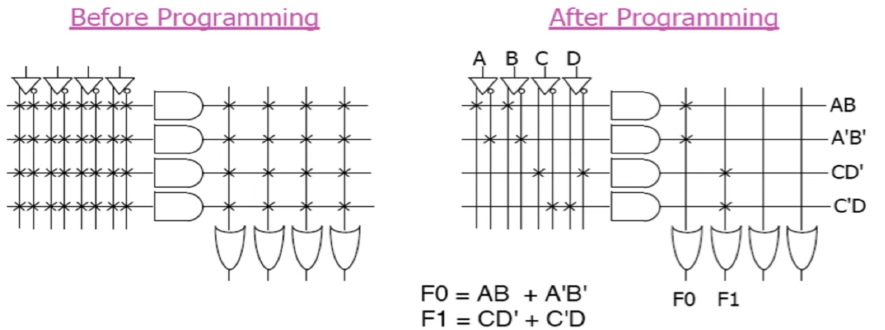
\includegraphics[width=0.86\linewidth]{bf.png}
\end{center}

\noindent\textbf{Esempio}: con 4 ingressi $A,B,C,D$ e 4 implicanti programmati
($AB$,~$A'B'$,~$CD'$,~$C'D$) si implementano le due funzioni:
\[
F_0 = AB + A'B' \qquad\quad F_1 = CD' + C'D = C \oplus D
\]

\defbox{
La \textbf{PLA} risparmia area rispetto alla ROM perché genera \emph{solo} gli implicanti
necessari e non tutti i $2^n$ mintermini. Il numero di righe del piano AND è uguale al
numero di implicanti distinti scelti (non a $2^n$).
}

% ======================================================================
\section{Multiplexer e demultiplexer}

\defbox{
\textbf{MUX} (multiplexer) = circuito digitale che funziona similmente a un selettore,
ma con $2^n$ ingressi, $n$ linee di controllo e 1 uscita.
}

\begin{fitcenter}
\begin{tikzpicture}[scale=0.88, every node/.style={scale=0.88}]
%--- MUX generico ---
\draw (0,0) rectangle (1.8,3.0);
\node at (0.9,1.5) {$2^n$};
% ingressi dati
\foreach \y in {2.5,2.0,1.0,0.5}{
  \draw[-latex] (-1.0,\y) -- (0,\y);
}
\node[left] at (-1.1,1.5) {ingressi};
\node[left,font=\scriptsize] at (-1.1,0.7) {$\vdots$};
% linee di controllo
\draw[-latex] (0.9,-0.8) -- (0.9,0) node[near start,right,font=\scriptsize]{$n$ linee di controllo};
% uscita
\draw[-latex] (1.8,1.5) -- (2.8,1.5) node[right]{uscita};

%--- Freccia =>  ---
\node at (4.2,1.5) {$\Rightarrow$};

%--- MUX 2:1 (con n=1) ---
\begin{scope}[xshift=5.0cm]
% corpo trapezoidale
\draw (0,0.3) -- (1.6,0.8) -- (1.6,2.2) -- (0,2.7) -- cycle;
\node[font=\scriptsize] at (0.75,1.5) {MUX};
% ingressi a0, a1
\draw[-latex] (-0.9,2.3) -- (0,2.3) node[midway,above,font=\scriptsize]{$a_0$};
\draw[-latex] (-0.9,0.7) -- (0,0.7) node[midway,above,font=\scriptsize]{$a_1$};
% selettore S
\draw[-latex] (0.75,-0.3) -- (0.75,0.3) node[near start,right,font=\scriptsize]{$S$};
% uscita
\draw[-latex] (1.6,1.5) -- (2.4,1.5) node[right,font=\scriptsize]{uscita};
\node[below=0.1cm,font=\scriptsize] at (0.75,-0.7) {con $n=1$};
\end{scope}

%--- Notazione ---
\begin{scope}[xshift=9.8cm]
\node[font=\small,align=center] at (0,1.8) {si chiama multiplexer};
\node[font=\small] at (0,1.3) {$2^n : m$};
\node[font=\scriptsize,color=noteteal] at (0.9,1.6) {$\leftarrow$ uscite};
\node[font=\scriptsize,color=noteteal] at (0.9,1.0) {$\leftarrow$ ingressi};
\end{scope}
\end{tikzpicture}
\end{fitcenter}

\medskip
\noindent\textbf{Ogni funzione a $n$ variabili può essere implementata con un
multiplexer $2^{n-1}:1$.}

\medskip
\noindent Consideriamo $F(a,b,c)=a\overline{b}+abc$ e costruiamo la
\textbf{tabella di verità funzionale} usando $a$ e $b$ come indirizzi del MUX\,4:1
($2^2=4$ ingressi) e $c$ come eventuale ingresso dati:

\begin{center}
\begin{minipage}{0.30\linewidth}
\begin{tabular}{cc|c}
\toprule
$a$ & $b$ & $D_i$ (MUX input)\\
\midrule
0 & 0 & 0\\
0 & 1 & 0\\
1 & 0 & 1\\
1 & 1 & $c$\\
\bottomrule
\end{tabular}
\end{minipage}%
\hspace{1.2cm}%
\begin{minipage}{0.45\linewidth}
\begin{tikzpicture}[scale=0.82, every node/.style={scale=0.82}]
% MUX 4:1 che implementa F(abc)
\draw (0,0) rectangle (1.8,3.4);
\node[font=\scriptsize] at (0.9,3.0) {MUX 4:1};
% ingressi dati
\draw[-latex] (-1.4,2.8) -- (0,2.8) node[midway,above,font=\tiny]{$D_{00}=0$};
\draw[-latex] (-1.4,2.1) -- (0,2.1) node[midway,above,font=\tiny]{$D_{01}=0$};
\draw[-latex] (-1.4,1.3) -- (0,1.3) node[midway,above,font=\tiny]{$D_{10}=1$};
\draw[-latex] (-1.4,0.6) -- (0,0.6) node[midway,above,font=\tiny]{$D_{11}=c$};
% selettori
\draw[-latex] (0.55,-0.5) -- (0.55,0) node[near start,left,font=\tiny]{$a$};
\draw[-latex] (1.25,-0.5) -- (1.25,0) node[near start,right,font=\tiny]{$b$};
% uscita
\draw[-latex] (1.8,1.7) -- (2.6,1.7) node[right,font=\tiny]{$F$};
\end{tikzpicture}
\end{minipage}
\end{center}

\medskip

\defbox{
\textbf{DEMUX} (demultiplexer) = circuito digitale opposto al MUX, con 1 ingresso,
$n$ linee di controllo e $2^n$ uscite.
}

\begin{fitcenter}
\begin{tikzpicture}[scale=0.88, every node/.style={scale=0.88}]
%--- DEMUX generico ---
\draw (0,0) rectangle (1.8,3.0);
\node at (0.9,1.5) {$2^n$};
% ingresso
\draw[-latex] (-1.0,1.5) -- (0,1.5) node[midway,above,font=\scriptsize]{ingresso $I$};
% linee di controllo
\draw[-latex] (0.9,-0.8) -- (0.9,0) node[near start,right,font=\scriptsize]{$n$ linee di controllo};
% uscite
\foreach \y in {2.5,2.0,1.0,0.5}{
  \draw[-latex] (1.8,\y) -- (2.8,\y);
}
\node[right,font=\scriptsize] at (2.9,1.5) {$2^n$ uscite};

%--- Freccia ---
\node at (4.4,1.5) {$\Rightarrow$};

%--- DEMUX 1:2 (con n=1) ---
\begin{scope}[xshift=5.2cm]
\draw (0,0.8) -- (0,2.2) -- (1.6,2.7) -- (1.6,0.3) -- cycle;
\node[font=\scriptsize] at (0.75,1.5) {DEMUX};
% ingresso
\draw[-latex] (-0.9,1.5) -- (0,1.5) node[midway,above,font=\scriptsize]{$D$};
% selettore
\draw[-latex] (0.75,-0.3) -- (0.75,0.8) node[near start,right,font=\scriptsize]{$S$};
% uscite
\draw[-latex] (1.6,2.3) -- (2.4,2.3) node[right,font=\scriptsize]{$o_1$};
\draw[-latex] (1.6,0.7) -- (2.4,0.7) node[right,font=\scriptsize]{$o_0$};
\node[below=0.1cm,font=\scriptsize] at (0.75,-0.7) {con $n=1$};
\end{scope}

%--- Notazione ---
\begin{scope}[xshift=10.0cm]
\node[font=\small,align=center] at (0,1.8) {si chiama multiplexer};
\node[font=\small] at (0,1.3) {$m : 2^n$};
\node[font=\scriptsize,color=noteteal] at (0.9,1.6) {$\leftarrow$ uscite};
\node[font=\scriptsize,color=noteteal] at (0.9,1.0) {$\leftarrow$ ingressi};
\end{scope}
\end{tikzpicture}
\end{fitcenter}

% ======================================================================
\section{Universal Shift Register (USR)}

\defbox{
\textbf{USR} (Universal Shift Register) = dispositivo che permette di mettere dati
in parallelo o in serie e di spostarli a destra e sinistra.
}

\begin{center}
\begin{tikzpicture}[scale=0.88, every node/.style={scale=0.88}]
% Tre celle n-1, n, n+1
\foreach \xi/\lab in {0/$n{-}1$, 2.8/$n$, 5.6/$n{+}1$}{
  \draw (\xi,0) rectangle (\xi+2.2,1.6);
  \node at (\xi+1.1,0.8) {\lab};
}
% Frecce rosse shift left (da destra a sinistra)
\draw[-latex,red,thick] (2.8,1.2) -- (2.2,1.2);
\draw[-latex,red,thick] (5.6,1.2) -- (5.0,1.2);
\draw[-latex,red,thick] (-0.7,1.2) -- (0,1.2);
\draw[-latex,red,thick] (7.8,1.2) -- (7.2,1.2) node[right,black,font=\scriptsize]{$\leftarrow$ shift left};
% Frecce blu/verde shift right (da sinistra a destra)
\draw[-latex,teal,thick] (2.2,0.4) -- (2.8,0.4);
\draw[-latex,teal,thick] (5.0,0.4) -- (5.6,0.4);
\draw[-latex,teal,thick] (-0.7,0.4) -- (0,0.4) node[right,black,font=\scriptsize]{};
\draw[-latex,teal,thick] (7.2,0.4) -- (7.9,0.4) node[right,black,font=\scriptsize]{shift right $\rightarrow$};
% Frecce verdi parallelo (dall'alto)
\foreach \xi in {1.1,3.9,6.7}{
  \draw[-latex,green!60!black,thick] (\xi,2.2) -- (\xi,1.6);
}
\node[above,font=\scriptsize,color=green!50!black] at (3.9,2.2) {caricamento parallelo};
% S0, S1
\draw[-latex] (-0.7,-0.5) -- (-0.7,0) node[below=0.4cm,font=\scriptsize]{$S_0$};
\draw[-latex] (0.0,-0.5) -- (0.0,0)  node[below=0.4cm,font=\scriptsize]{$S_1$};
\end{tikzpicture}
\end{center}

\noindent\textbf{Vediamo come implementare ogni singola unità dell'USR.}

\medskip
\noindent Possiamo guidare le quattro funzioni con un \textbf{MUX 4:1} (2 indirizzi):
HOLD, SHIFT LEFT, SHIFT RIGHT, DATA IN.

\begin{center}
\begin{minipage}{0.28\linewidth}
\begin{tabular}{cc|l}
\toprule
$S_1$ & $S_0$ & Funzione\\
\midrule
0 & 0 & hold\\
0 & 1 & shift right\\
1 & 0 & shift left\\
1 & 1 & data in\\
\bottomrule
\end{tabular}
\end{minipage}%
\hspace{0.8cm}%
\begin{minipage}{0.58\linewidth}
\begin{tikzpicture}[scale=0.85, every node/.style={scale=0.85}]
%--- MUX 4:1 ---
\draw (1.5,0) rectangle (3.0,4.0);
\node[font=\scriptsize\bfseries] at (2.25,3.6) {M};
\node[font=\scriptsize\bfseries] at (2.25,3.2) {U};
\node[font=\scriptsize\bfseries] at (2.25,2.8) {X};
% ingressi dati
\draw[-latex] (0,3.5) -- (1.5,3.5) node[midway,above,font=\tiny]{$Q_n$\;\;(00)};
\draw[-latex] (0,2.5) -- (1.5,2.5) node[midway,above,font=\tiny]{$Q_{n-1}$\;(10)};
\draw[-latex] (0,1.5) -- (1.5,1.5) node[midway,above,font=\tiny]{$Q_{n+1}$\;(01)};
\draw[-latex] (0,0.5) -- (1.5,0.5) node[midway,above,font=\tiny]{$I_n$\;\;\;(11)};
% selettori
\draw[-latex] (1.9,-0.6) -- (1.9,0) node[near start,left,font=\tiny]{$S_1$};
\draw[-latex] (2.6,-0.6) -- (2.6,0) node[near start,right,font=\tiny]{$S_0$};
%--- uscita MUX -> DFF ---
\draw[-latex] (3.0,2.0) -- (4.0,2.0) node[midway,above,font=\tiny]{$D_n$};
%--- DFF ---
\draw (4.0,1.2) rectangle (5.8,2.8);
\node[font=\scriptsize] at (4.9,2.4) {$D$\quad$Q_n$};
% triangolo clock
\draw (4.0,1.5) -- (4.3,1.7) -- (4.0,1.9);
\draw[-latex] (4.9,0.5) -- (4.9,1.2) node[near start,right,font=\tiny]{CLK};
% CLR
\draw[-latex] (4.3,0.5) -- (4.3,1.2) node[near start,left,font=\tiny]{CLR};
% uscita Q_n
\draw[-latex] (5.8,2.0) -- (6.6,2.0) node[right,font=\scriptsize]{$Q_n$};
% feedback Q_n -> input 00
\draw (6.3,2.0) -- (6.3,4.8) -- (-0.4,4.8) -- (-0.4,3.5) -- (0,3.5);
\node[right,font=\tiny,color=noteteal] at (6.6,2.5) {$=$ USR};
\end{tikzpicture}
\end{minipage}
\end{center}

\noindent\textit{Se CLR = 1 si effettua un RESET a 0 sincrono.}

% ======================================================================
\subsection{Implementazione a 4 bit per trasmissione PISO}

\begin{fitcenter}
\begin{tikzpicture}[scale=0.8, every node/.style={scale=0.8}]
% 4 celle USR in cascata
\foreach \i/\xi/\lin in {0/0/$I_0$, 1/2.6/$I_1$, 2/5.2/$I_2$, 3/7.8/$I_3$}{
  \draw (\xi,0.4) rectangle (\xi+2.2,2.4);
  \node[font=\scriptsize] at (\xi+1.1,1.4) {$Q_{\i}$};
  % Ingresso parallelo dall'alto
  \draw[-latex] (\xi+1.1,3.0) -- (\xi+1.1,2.4) node[above=0.5cm,font=\tiny]{\lin};
  % S0 S1 dal basso
  \draw[-latex] (\xi+0.6,-0.3) -- (\xi+0.6,0.4) node[below=0.3cm,font=\tiny]{$S_0$};
  \draw[-latex] (\xi+1.5,-0.3) -- (\xi+1.5,0.4) node[below=0.3cm,font=\tiny]{$S_1$};
}
% collegamento in cascata: Q_i uscita -> Q_{i+1} ingresso seriale
\draw[-latex] (2.2,1.4) -- (2.6,1.4);
\draw[-latex] (4.8,1.4) -- (5.2,1.4);
\draw[-latex] (7.4,1.4) -- (7.8,1.4);
% input sinistro LI (=LSI)
\draw[-latex] (-0.9,1.8) -- (0,1.8) node[midway,above,font=\tiny]{$L_I$};
% input destro RI (=RSI)
\draw[-latex] (10.9,1.0) -- (10.0,1.0) node[midway,above,font=\tiny]{$R_I$};
% uscita sinistra L0
\draw[-latex] (0,1.0) -- (-0.9,1.0) node[left,font=\tiny]{$L_0$};
% uscita destra R0
\draw[-latex] (10.0,1.8) -- (10.9,1.8) node[right,font=\tiny]{$R_0$};
% CLK comune
\draw[-latex] (-1.2,-1.0) -- (-1.2,-1.4) -- (9.8,-1.4);
\foreach \xi in {1.1,3.7,6.3,8.9}{
  \draw[-latex] (\xi,-1.4) -- (\xi,0.4);
}
\node[left,font=\tiny] at (-1.2,-1.0) {CLK};
% CLR comune
\draw[-latex] (-0.6,-0.9) -- (-0.6,-1.9) -- (9.7,-1.9);
\foreach \xi in {0.8,3.4,6.0,8.6}{
  \draw (\xi,-1.9) -- (\xi,-0.3);
  \draw[-latex] (\xi,-0.3) -- (\xi,0.4);
}
\node[left,font=\tiny] at (-0.6,-0.9) {CLR};
% Legenda
\node[align=left,font=\tiny] at (10.5,-0.4) {$L_I = \text{LSI}$\\$R_I = \text{RSI}$\\$L_0 = \text{LSD}$\\$R_0 = \text{RSO}$};
\end{tikzpicture}
\end{fitcenter}

\noindent Il circuito permette 4 modalità operative selezionate da $S_1 S_0$:
caricamento parallelo, shift left (seriale verso sinistra), shift right (seriale verso
destra) e hold.

\subsection{Applicazione: trasmissione seriale Sender--Receiver}

\begin{center}
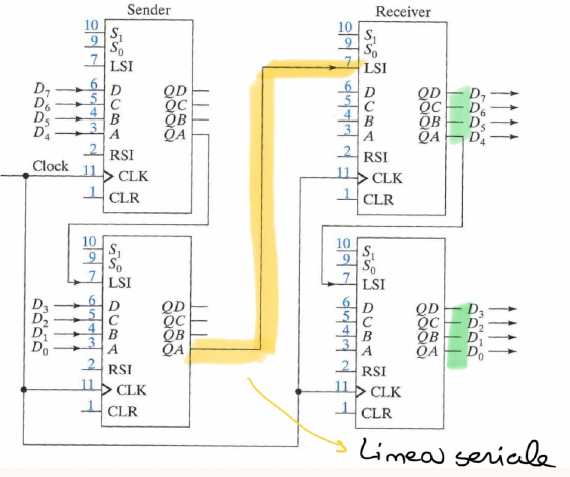
\includegraphics[width=0.78\linewidth]{crl.png}
\end{center}

\noindent Il flusso dell'operazione è:
\[
\text{Caricamento nel Sender di }D_i
\;\xrightarrow{\text{shift}}\;
\text{Trasmissione sulla linea seriale}
\;\xrightarrow{\text{shift}}\;
\text{Lettura sulle uscite del Receiver}
\]

% ======================================================================
\section{Vincoli temporali dell'USR e Jitter}

\noindent La \textbf{massima frequenza del clock} per un USR corrisponde al
\textbf{minimo periodo del clock}:

\[
\boxed{T_{\text{CLK,min}} = T_{\text{setup}} + T_{\text{propag}} + T_{\text{lc}} + T_{\text{jitter}}}
\]

\begin{center}
\begin{tikzpicture}[scale=0.9, every node/.style={scale=0.9}]
% Linea temporale con le 4 componenti
\draw[-latex] (0,0) -- (9.5,0) node[right]{$t$};
% Segmenti
\draw[thick,teal]   (0,0)   -- (2.0,0);
\draw[thick,orange] (2.0,0) -- (4.2,0);
\draw[thick,blue]   (4.2,0) -- (6.5,0);
\draw[thick,red]    (6.5,0) -- (8.5,0);
% tick marks
\foreach \x in {0,2.0,4.2,6.5,8.5}{
  \draw (\x,0.15) -- (\x,-0.15);
}
% etichette
\node[above,font=\scriptsize,color=teal]   at (1.0,0.1) {$T_{\text{propag}}$};
\node[above,font=\scriptsize,color=orange] at (3.1,0.1) {$T_{\text{lc}}$};
\node[above,font=\scriptsize,color=blue]   at (5.35,0.1) {$T_{\text{setup}}$};
\node[above,font=\scriptsize,color=red]    at (7.5,0.1) {$T_{\text{jitter}}$};
% frecce-descrizione
\node[below,font=\tiny,color=teal,align=center]   at (1.0,-0.3) {ritardo\\CLK$\to Q$ nel FF};
\node[below,font=\tiny,color=orange,align=center] at (3.1,-0.3) {ritardo logica\\comb.\ (MUX)};
\node[below,font=\tiny,color=blue,align=center]   at (5.35,-0.3) {stabilità per\\CLK successivo};
\node[below,font=\tiny,color=red,align=center]    at (7.5,-0.3) {jitter del CLK};
\end{tikzpicture}
\end{center}

\defbox{
\textbf{Jitter del CLK} = $\Delta_{\max}$ fra gli istanti di arrivo dei fronti di clock
che dovrebbero giungere \emph{contemporaneamente} a tutti i componenti del circuito, ma
che in pratica non lo fanno a causa di variazioni fisiche (disadattamenti di linea,
rumore, disomogeneità dei percorsi).
}


% ======================================================================
\chapter{Conversione Digitale--Analogica e Analogica--Digitale}
\textit{(15 maggio 2026)}

% ======================================================================
\section{Conversione digitale $\leftrightarrow$ analogica}

Il processo di acquisizione e ricostruzione del segnale si articola in due fasi:

\begin{center}
\begin{tikzpicture}[scale=0.85, every node/.style={scale=0.85},
  box/.style={draw, minimum width=1.6cm, minimum height=0.8cm, align=center, font=\small},
  arr/.style={-latex,thick}]

% --- segnale analogico campionato ---
\node[font=\small] at (0,2.2) {$\Delta V$};
\draw[arr] (-0.2,0) -- (4.2,0); \node[right,font=\scriptsize] at (4.2,0) {$t$};
\draw[arr] (0,-0.2) -- (0,2.0);
\foreach \x/\h in {0.5/1.2, 1.0/1.6, 1.5/1.8, 2.0/1.5, 2.5/1.0, 3.0/0.8, 3.5/1.3}{
  \draw[blue,thick] (\x,0) -- (\x,\h);
  \fill[blue] (\x,\h) circle (2pt);
}
\node[above,font=\scriptsize] at (2.0,2.2) {campionamenti $V(t_i)$};

% --- blocchi Sensore -> ADC ---
\node[box] (sens) at (5.8,0.9) {Sensore};
\node[box] (adc)  at (7.8,0.9) {ADC};
\draw[arr] (4.5,0.9) -- (sens.west);
\draw[arr] (sens.east) -- (adc.west);
\draw[arr] (adc.south) -- ++(0,-0.5) node[below,font=\scriptsize,align=center]{convertitore\\analogico$\to$digitale};
\draw[arr] (adc.east)  -- ++(1.0,0);

% --- segnale ricostruito ---
\begin{scope}[xshift=9.5cm]
\node[font=\small] at (0,2.2) {$\Delta V$};
\draw[arr] (-0.2,0) -- (4.2,0); \node[right,font=\scriptsize] at (4.2,0) {$t$};
\draw[arr] (0,-0.2) -- (0,2.0);
\foreach \x/\h in {0.5/1.2, 1.0/1.6, 1.5/1.8, 2.0/1.5, 2.5/1.0, 3.0/0.8, 3.5/1.3}{
  \fill[blue] (\x,\h) circle (2pt);
}
\draw[blue,thick,domain=0.5:3.5,samples=60] plot(\x,{1.5+0.4*sin(3.14159*\x r)+0.3*cos(6.28*\x r)});
\node[above,font=\scriptsize] at (2.0,2.3) {estrapolazioni lineari};
\node[below,font=\scriptsize] at (2.0,-0.3) {dopo l'elaborazione del segnale};
\end{scope}
\end{tikzpicture}
\end{center}

\noindent Il quesito è: cosa succede fra il campionamento e la ricostruzione? La risposta è
\textbf{sample and hold} $\to$ \textbf{convertitore analogico$\to$digitale} $\to$ \textbf{convertitore digitale$\to$analogico}, in sintesi:
\[
\text{Sensore} \;\xrightarrow{\text{ADC}}\; \text{elaborazione digitale} \;\xrightarrow{\text{DAC}}\; \text{uscita analogica}
\]

\noindent Definizioni di base:
\begin{itemize}[leftmargin=1.5em]
    \item $n_{(\cdot)}$ = numero che dipende dai bit disponibili;
    \item $\Delta V$ = \textbf{granularità}, ovvero il passo minimo distinguibile;
    \item $V_{\text{ref}}$ = valore massimo attingibile.
\end{itemize}

\defbox{
\textbf{Funzione di trasferimento di un ADC}: $\quad n_{\text{out}} = V_{\text{in}}/\Delta V$\\[0.3em]
\textbf{Funzione di trasferimento di un DAC}: $\quad V_{\text{out}} = n_{\text{in}} \cdot \Delta V$
}

% ======================================================================
\section{Caratteristiche del DAC}

\defbox{
\textbf{Precisione} = determinata dal numero di bit e dall'intervallo di tensioni:
\[
V_{\text{out}} = n_{\text{in}} \cdot \Delta V
\]
Ad esempio, con $n$-bit $= 3$ e $\Delta V = 1\,\text{V}$:
$n_{\text{in}} \in [0,\, 2^3{-}1] \;\Rightarrow\; V_{\text{out}} \in [0,\, 2^3{-}1]\,\text{V}$.
}

\noindent La velocità di conversione è molto importante e dipende da diversi fattori: tipo di
assestamento, architettura e numero di bit. Le tre principali sorgenti di errore nel DAC sono:

\begin{center}
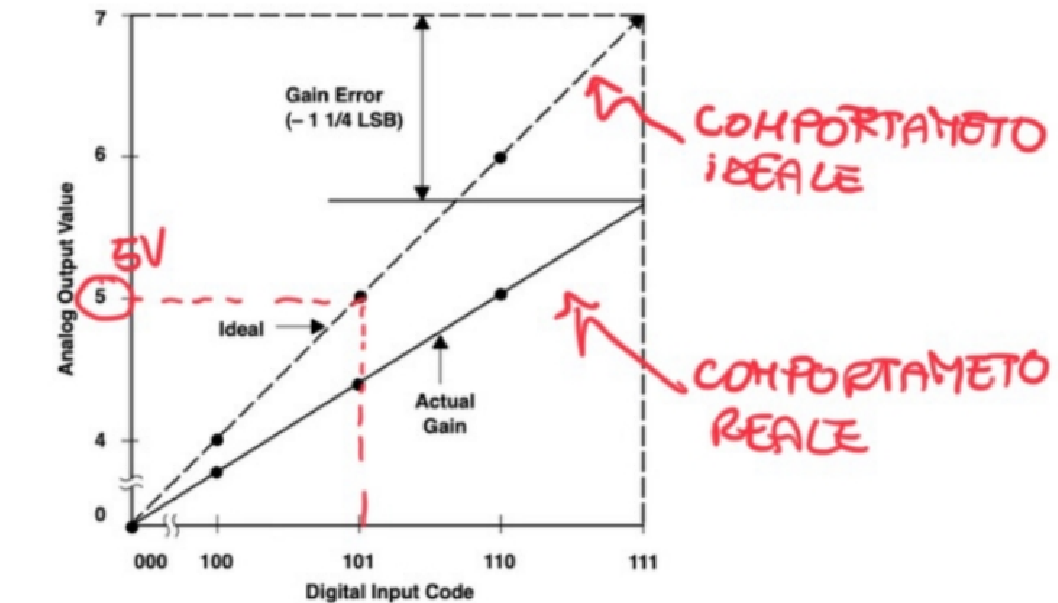
\includegraphics[width=0.32\linewidth]{err_g.png}\hfill
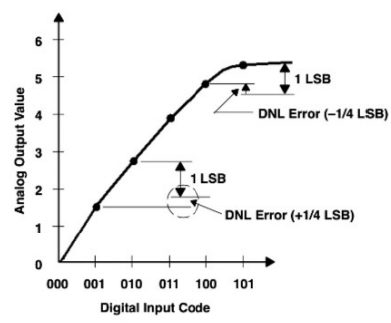
\includegraphics[width=0.32\linewidth]{n_lin.png}\hfill
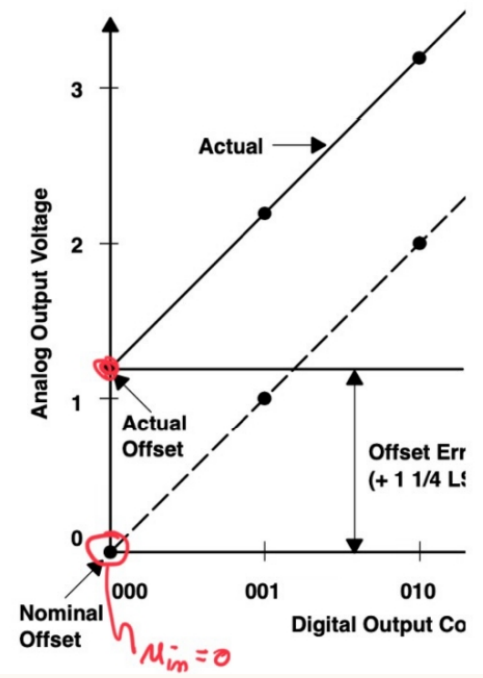
\includegraphics[width=0.32\linewidth]{er_nlin.png}
\end{center}

% ======================================================================
\section{DAC a sommatore}

L'architettura più semplice di DAC è il \textbf{DAC a sommatore pesato}: si usa un
amplificatore operazionale invertente con resistenze pesate $R_i = R/2^i$ per ciascun
bit. Le resistenze di ingresso sono collegate a $V_{\text{ref}}$ (bit $a_i=1$) o a massa
(bit $a_i=0$) tramite uno switch digitale per ciascun bit.

\begin{center}
\begin{circuitikz}[scale=0.85, every node/.style={scale=0.85}, american voltages]

\node[op amp, noinv input up] (OA) at (4.0,0) {};

% Resistenza di retroazione R
\draw (OA.out) -- ++(0,1.4) to[R, l=$R$] ++(-2.4,0) -- ++(0,-0.55);

% Nodo sommatore (ingresso invertente)
\draw (OA.-) -- ++(-0.4,0) coordinate (suma);

% Bit a0 (MSB)
\draw (suma) -- ++(0,+0.9) to[R, l=$R$, -*] ++(-1.8,0)
      node[left]{$V_{\text{ref}}$} node[above right,font=\scriptsize]{$a_0$ (MSB)};

% Bit a1
\draw (suma) to[R, l=$2R$, -*] ++(-1.8,0)
      node[left]{$V_{\text{ref}}$} node[above right,font=\scriptsize]{$a_1$};

% Bit a2 (LSB)
\draw (suma) -- ++(0,-0.9) to[R, l=$4R$, -*] ++(-1.8,0)
      node[left]{$V_{\text{ref}}$} node[above right,font=\scriptsize]{$a_2$ (LSB)};

% Massa sul + dell'OA
\draw (OA.+) -- ++(0,-0.4) node[ground]{};

% Uscita
\draw (OA.out) -- ++(0.8,0) node[right]{$V_{\text{out}}$};

\end{circuitikz}
\end{center}

\noindent\textit{Nota}: ogni ramo $a_i$ è collegato a $V_{\text{ref}}$ tramite uno switch
digitale, che si chiude o si apre (collegando in alternativa a massa) a seconda del valore
del bit; il simbolo del cursore $\updownarrow$ negli appunti originali indica proprio questo
switch a monte dell'ingresso invertente.

\noindent La formula di uscita si ricava dalla sovrapposizione degli effetti:
\[
V_{\text{out}} = -V_{\text{ref}}\!\left(\frac{R}{R_0}+\frac{R}{R_1}+\frac{R}{R_2}\right)
\]
Se si pone $R_i = R/2^i$, allora $R/R_i = 2^i$ e quindi:
\[
\boxed{V_{\text{out}} = -V_{\text{ref}}\sum_i 2^i}
\]
Considerando gli switch digitali, ogni bit $a_i$ vale 0 (collegamento a terra) oppure 1
(collegamento a $V_{\text{ref}}$):
\[
\boxed{V_{\text{out}} = -V_{\text{ref}}\sum_i a_i\,2^i}
\]

\medskip
\noindent\textbf{Limite pratico}: supponendo 10 bit, $R_i = 100\,\text{k}\Omega/2^i$.
Se la tolleranza è $\sigma_0 = 1\%$ e $R_0 = 1\,\text{k}\Omega$, i bit meno significativi
vengono persi perché il loro valore di resistenza scende sotto la tolleranza stessa
($R_i < \sigma_0$). Questo DAC è quindi utilizzabile solo con pochi bit; altrimenti non è
sufficientemente preciso.

% ======================================================================
\section{DAC R-2R Ladder}

Per avere un DAC più preciso si usa la tecnica \textbf{R-2R Ladder}, che genera pesi
binari per i bit usando solo due valori di resistenza ($R$ e $2R$):

\begin{center}
\begin{circuitikz}[scale=0.85, every node/.style={scale=0.85}, american voltages]

\coordinate (n0) at (0,6.0);   % MSB (bit 0)
\coordinate (n1) at (0,4.0);   % bit 1
\coordinate (n2) at (0,2.0);   % bit 2
\coordinate (n3) at (0,0.0);   % LSB (bit 3)

% Rami 2R orizzontali verso Vref/switch
\foreach \y/\lab in {6.0/0, 4.0/1, 2.0/2, 0.0/3}{
  \draw (0,\y) to[R, l=$2R$] (-2.4,\y);
  \draw[-latex] (-2.4,\y) -- (-3.2,\y) node[left,font=\scriptsize]{$a_{\lab}$};
}

% Rami R verticali tra i nodi
\draw (0,6.0) to[R, l=$R$] (0,4.0);
\draw (0,4.0) to[R, l=$R$] (0,2.0);
\draw (0,2.0) to[R, l=$R$] (0,0.0);

% Terminazione a massa
\draw (0,0.0) to[R, l=$R$] (0,-1.6) node[ground]{};

% Linea di uscita verso OA
\draw (0,6.0) -- (1.0,6.0) coordinate (vout_line);

% OpAmp
\node[op amp, noinv input up] (OA) at (3.5,5.2) {};
\draw (vout_line) -- (OA.-);
\draw (OA.+) -- ++(0,-0.4) node[ground]{};
\draw (OA.out) -- ++(0,1.2) to[R, l=$2R$] ++(-2.6,0) -- ++(0,-0.6);
\draw (OA.out) -- ++(0.8,0) node[right]{$V_{\text{out}}$};

\node[right,font=\scriptsize,color=noteblue] at (0.2,6.0) {MSB};
\node[right,font=\scriptsize,color=noteblue] at (0.2,0.0) {LSB};

\end{circuitikz}
\end{center}

\noindent Ogni bit $a_i$ contribuisce all'uscita con un peso binario:
\[
a_i \;\longrightarrow\; V_{\text{out},i} = -\frac{V_{\text{ref}}}{2^{i+1}}
\qquad\Rightarrow\quad
\text{i pesi sono } \frac{1}{2},\,\frac{1}{4},\,\frac{1}{8},\,\frac{1}{16},\ldots
\]
\[
\boxed{V_{\text{out}} = -V_{\text{ref}}\sum_i \frac{a_i}{2^{i+1}}}
\]

\noindent\textbf{Esempio}: con 4 bit, ingresso $1010_2$ e $V_{\text{ref}} = 8\,\text{V}$:
\[
V_{\text{out}} = -8\!\left(\frac{1}{2}+\frac{1}{8}\right) = -8 \cdot \frac{5}{8} = -5\,\text{V}
\]

% ======================================================================
\section{Caratteristiche dell'ADC}

\begin{itemize}[leftmargin=1.5em]
    \item \textbf{Accuratezza} = insieme di tutte le sorgenti di errore, errore di
          quantizzazione compreso.
    \item \textbf{Errore di quantizzazione} = dipende dal tipo di ADC ed è dovuto alla
          discretizzazione del segnale durante la conversione; di solito vale $1$ LSB
          oppure $0{,}5$ LSB.
    \item \textbf{Tempo di conversione} e \textbf{funzionamento} sono altre caratteristiche
          importanti dell'ADC.
\end{itemize}

\noindent Analogamente al DAC, anche l'ADC presenta tre principali tipi di errore rispetto
al comportamento ideale:

\begin{center}
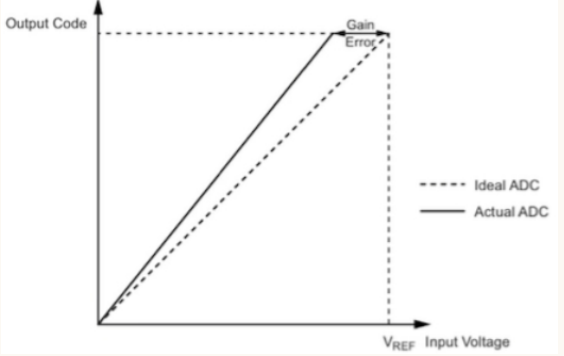
\includegraphics[width=0.32\linewidth]{err_g2.png}\hfill
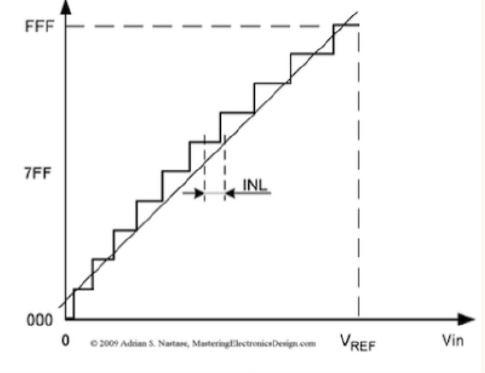
\includegraphics[width=0.32\linewidth]{n_lin2.png}\hfill
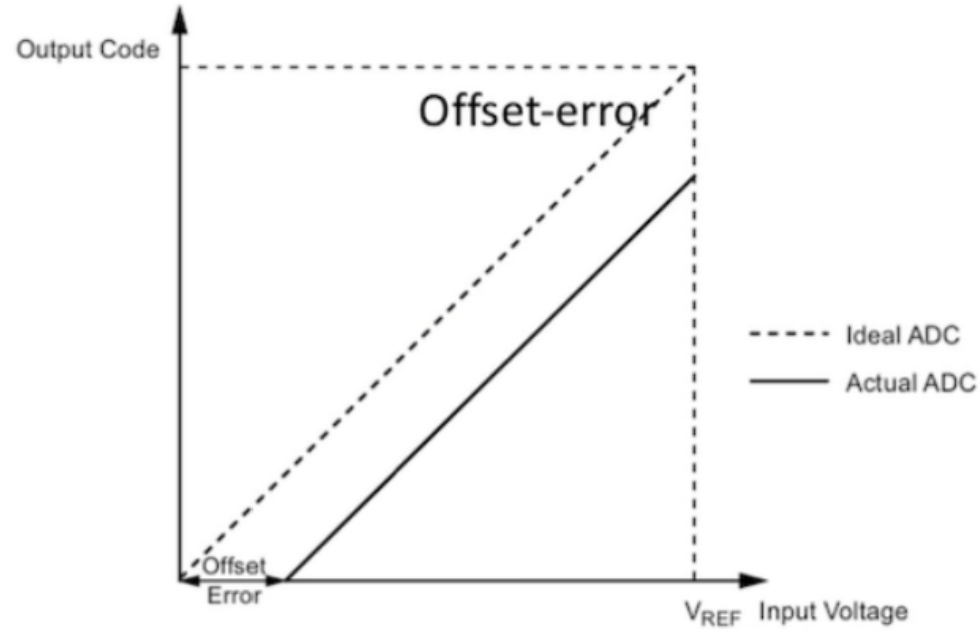
\includegraphics[width=0.32\linewidth]{er_nlin2.png}
\end{center}

% ======================================================================
\chapter{Convertitori Analogico-Digitali (ADC)}
\textit{(15 maggio 2026 -- cont.)}

% ---------- BLOCCO 1: ADC a gradinata ----------
\section{ADC a gradinata}

\noindent
\begin{minipage}[t]{0.42\textwidth}
    \vspace{0pt}
    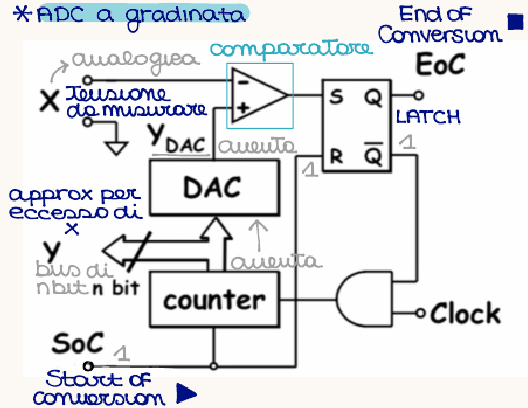
\includegraphics[width=\textwidth]{11.png}
\end{minipage}%
\hfill
\begin{minipage}[t]{0.55\textwidth}
    \vspace{0pt}
    \begin{itemize}[leftmargin=1em]
        \item \textbf{Funzionamento del comparatore}: finché $X > Y_{DAC}$ il conteggio procede; appena $Y_{DAC} \geq X$ il comparatore cambia stato $\rightarrow$ il latch RS blocca il \texttt{CLK} e il \texttt{counter}.
        \item \textbf{Funzionamento del contatore}: genera $N_{in_2} \rightarrow N_{in_0}$ e aumenta la tensione.
        \item La granularità dipende da $V_{REF}$ del DAC (cioè il $\Delta V$ con cui aumenta).
        \item Asintoticamente questo ADC deve fare $2^{n}$ confronti, dove $n$ sono i livelli del DAC:
        \begin{equation*}
            T_{conv} = 2^{n} \, T_{CLK}
        \end{equation*}
    \end{itemize}
\end{minipage}

\vspace{1.5em}

% ---------- BLOCCO 2: ADC SAR ----------
\section{ADC ad approssimazioni successive (SAR)}

\noindent
\begin{minipage}[t]{0.42\textwidth}
    \vspace{0pt}
    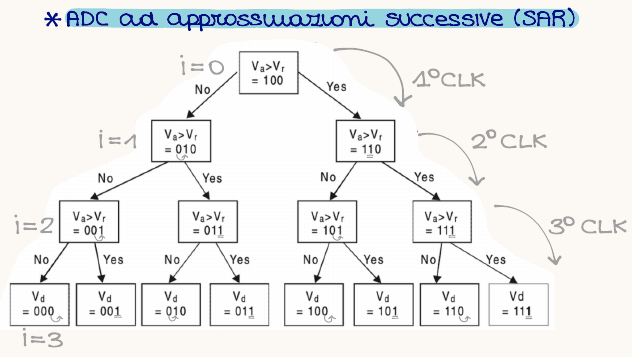
\includegraphics[width=\textwidth]{22.png}
\end{minipage}%
\hfill
\begin{minipage}[t]{0.55\textwidth}
    \vspace{0pt}
    \begin{itemize}[leftmargin=1em]
        \item Il valore di tensione da misurare si confronta con i successivi.
        \item Ogni conversione avviene in un ciclo di \texttt{CLK}. Se $n_{bit}=3$ ci sono 3 cicli.
        \item \textbf{Yes}: metto un 1 nella posizione $i+1$ se passo da $i$ a $i+1$.
        \item \textbf{No}: sposto l'1 dalla posizione $i$ alla posizione $i+1$ passando da $i$ a $i+1$.
        \item È una ricerca binaria: i confronti sono $n$, quindi:
        \begin{equation*}
            T_{conv} = n \, T_{CLK}
        \end{equation*}
        \item Funzionamento specifico alla pagina successiva.
    \end{itemize}
\end{minipage}

\vspace{1.5em}

% ---------- BLOCCO 3: FLASH ADC ----------
\section{Flash ADC}

\noindent
\begin{minipage}[t]{0.42\textwidth}
    \vspace{0pt}
    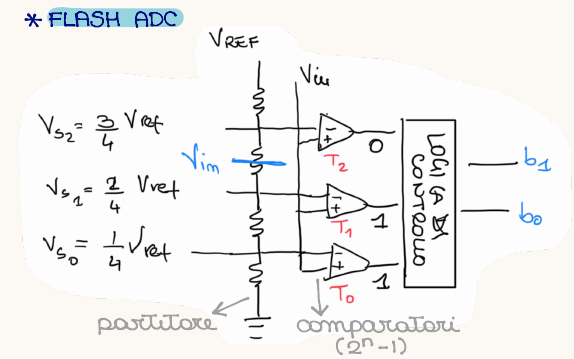
\includegraphics[width=\textwidth]{33.png}
\end{minipage}%
\hfill
\begin{minipage}[t]{0.55\textwidth}
    \vspace{0pt}
    \begin{itemize}[leftmargin=1em]
        \item La tensione viene confrontata contemporaneamente con $n$ valori; poi un circuito combinatorio converte le uscite dei confronti in binario (1 = valori coperti da $V_{in}$; 0 = valori più alti di $V_{in}$).
        \item Un confronto: istantaneo (fatto in parallelo) $\Rightarrow$ è il più veloce.
        \item La precisione è però molto minore di quella degli altri (servono tante resistenze, con i problemi già discussi).
        \item Risolvo coi mintermini, sapendo che se $j < i < k$ e $T_i = 1$ allora $T_j = 1$ e $T_k = 0$:
        \begin{align*}
            b_0 &= T_2 + T_0 \cdot T_1 \\
            b_1 &= T_2 + T_1 \cdot \overline{T_2}
        \end{align*}
    \end{itemize}
\end{minipage}

\vspace{1.5em}

\section{Osservazioni generali}
\begin{itemize}[leftmargin=1.5em]
    \item L'errore di quantizzazione è pari a $0{,}5 \, V_{REF}/2^{n}$.
\end{itemize}

\section{ADC dell'AD2}
\begin{itemize}[leftmargin=1.5em]
    \item Ci sono \SI{14}{bit} $\Rightarrow 2^{14}$ possibili valori.
    \item Se scelgo la scala \SI{0.5}{\volt}/div l'intervallo in cui misuro è $(0, 0{,}5 \cdot 10)\,\si{\volt} = (0,5)\,\si{\volt}$, e la quantizzazione è:
    \begin{equation*}
        \frac{\SI{5}{\volt}}{2^{14}} \approx \SI{0.3}{\milli\volt}
    \end{equation*}
\end{itemize}

% ============================================================
% ADC ad approssimazioni successive (SAR) - Circuito a 3 bit
% Spiegazione dettagliata basata sulle slide del corso
% ============================================================

\subsection{ADC ad approssimazioni successive (SAR): analisi del circuito a 3 bit}

Il convertitore analogico--digitale ad \emph{approssimazioni successive} (in inglese \textbf{S}uccessive \textbf{A}pproximation \textbf{R}egister, SAR) determina il codice digitale corrispondente ad una tensione analogica $V_a$ eseguendo un confronto ``dicotomico'' bit a bit, a partire dal bit più significativo (MSB) fino al meno significativo (LSB). Il circuito visto a lezione realizza un SAR a 3 bit ed è composto dai seguenti blocchi funzionali:

\begin{itemize}
    \item \textbf{Ring Counter} (registro a scorrimento circolare) costituito da 5 flip-flop $S_0,\dots,S_4$: genera, un colpo di clock alla volta, un impulso che si sposta da uno stadio al successivo. Questo impulso scandisce il tempo di test di ciascun bit (MSB $\to$ LSB) e determina quando la conversione è terminata.
    \item \textbf{Registro dei bit di prova} composto da 3 flip-flop $Q_2, Q_1, Q_0$ (MSB $\to$ LSB): contiene, istante per istante, il codice binario di tentativo.
    \item \textbf{DAC} (convertitore digitale--analogico): converte il codice presente in $Q_2Q_1Q_0$ nella tensione di confronto $V_{DAC}$.
    \item \textbf{Comparatore analogico}: confronta $V_a$ (tensione incognita da convertire) con $V_{DAC}$.
    \item \textbf{Logica combinatoria (porte AND/OR)}: in base all'uscita del comparatore e allo stadio attivo del Ring Counter, decide se mantenere a 1 oppure resettare a 0 il bit appena testato.
\end{itemize}

\`E importante notare che il Ring Counter e il registro dei bit di prova lavorano \emph{in parallelo}: mentre il Ring Counter ``punta'' al bit che si sta testando in quel colpo di clock, il registro $Q_2Q_1Q_0$ contiene il codice di prova corrente, che viene aggiornato bit dopo bit.

\bigskip
\subsubsection{Fase 1 -- Inizializzazione (prima del primo fronte di clock)}

Prima dell'arrivo del primo fronte di clock il circuito viene inizializzato nel seguente modo:

\begin{enumerate}
    \item Si invia il segnale di \texttt{CLEAR} (attivo basso) contemporaneamente a tutti i flip-flop del registro dati $Q_2,Q_1,Q_0$: tutte le uscite vengono forzate a 0.
    \item Contemporaneamente si setta $S_0=1$ (primo stadio del Ring Counter) tramite ingresso asincrono, mentre tutti gli altri stadi $S_1,\dots,S_4$ vengono inizializzati a 0.
    \item Poich\'e il registro dati è tutto a 0, l'ingresso del DAC è $000$, quindi l'uscita del DAC è
    \[
        V_{DAC} = 0\ \text{V}.
    \]
\end{enumerate}

Lo stato del sistema subito prima del primo fronte di clock è dunque:
\[
(S_4 S_3 S_2 S_1 S_0) = (0\,0\,0\,0\,1), \qquad (Q_2 Q_1 Q_0) = (0\,0\,0), \qquad V_{DAC}=0\text{ V}.
\]

\bigskip
\subsubsection{Fase 2 -- Subito dopo il primo fronte di clock}

Al primo fronte di clock accadono due cose contemporaneamente:

\begin{itemize}
    \item Il Ring Counter avanza di uno stadio: $S_0 \to 0$, $S_1 \to 1$. Questo impulso su $S_1$ abilita la scrittura del bit più significativo $Q_2$.
    \item La logica combinatoria pone \emph{a priori} $Q_2 = 1$ (si ``prova'' il bit più significativo settandolo a 1): il nuovo codice di prova è $Q_2Q_1Q_0 = 100$.
\end{itemize}

Con il nuovo codice in ingresso, il DAC produce la tensione corrispondente a $n=4$ (in decimale):
\[
V_{DAC} = V(n{=}4) \quad \text{(tensione corrispondente al codice \texttt{100})}.
\]

A questo punto il comparatore confronta $V_a$ con $V_{DAC}$: il risultato di questo confronto sarà disponibile e utilizzato al fronte di clock \emph{successivo} per decidere se mantenere $Q_2=1$ oppure resettarlo a 0.

\bigskip
\subsubsection{Esempio numerico}

Supponiamo che il DAC abbia una risoluzione $\Delta V = 1\text{ V}$ sull'intervallo $[0,7]\text{ V}$ (3 bit, 8 livelli) e che la tensione incognita sia
\[
V_a = 5.5\text{ V}.
\]

Dopo il primo fronte di clock il registro contiene $Q_2Q_1Q_0=100$, quindi
\[
V_{DAC} = 4\text{ V}.
\]

Il comparatore verifica se $V_a > V_{DAC}$ (equivalentemente, se $V_a$ supera la metà del fondo scala, $V_{max}/2$):
\[
V_a = 5.5\text{ V} > V_{DAC}=4\text{ V} \quad\Longrightarrow\quad \text{SI}.
\]

Poich\'e il confronto ha dato esito positivo, il bit $Q_2$ appena testato viene \textbf{mantenuto a 1} (l'approssimazione ``per difetto'' era corretta: la tensione reale è maggiore di quella generata dal DAC con quel bit a 1, quindi quel bit resta valido nel codice finale).

\bigskip
\subsubsection{Fase 4 -- Subito dopo il secondo fronte di clock}

Al secondo fronte di clock:

\begin{itemize}
    \item Il Ring Counter avanza ancora: $S_1\to 0$, $S_2\to 1$. L'impulso su $S_2$ abilita ora la scrittura del bit successivo $Q_1$.
    \item Il risultato del confronto precedente (esito ``SI'', $V_a>V_{DAC}$) viene usato dalla logica combinatoria per \textbf{confermare} $Q_2=1$ definitivamente.
    \item Contemporaneamente si prova il nuovo bit ponendo $Q_1=1$: il codice di prova diventa $Q_2Q_1Q_0 = 110$.
\end{itemize}

Il DAC aggiorna quindi la propria uscita al nuovo codice:
\[
V_{DAC} = 4\text{ V} + 2\text{ V} = 6\text{ V}.
\]

Si esegue un nuovo confronto:
\[
V_a = 5.5\text{ V} < V_{DAC} = 6\text{ V} \quad\Longrightarrow\quad \text{esito negativo}.
\]

Questa volta il bit appena provato ($Q_1$) risulter\`a, al fronte di clock successivo, \textbf{resettato a 0} (il DAC ha superato $V_a$, quindi quel bit non pu\`o essere 1 nel codice finale): il codice torna a $100$ per quanto riguarda $Q_2Q_1$, e si passer\`a a testare l'ultimo bit $Q_0$.

\bigskip
\subsubsection{Algoritmo generale (n bit)}

Il procedimento si generalizza a un ADC-SAR a $n$ bit come segue: per ogni bit, dal MSB al LSB,

\begin{enumerate}
    \item il Ring Counter abilita la scrittura del bit corrente;
    \item la logica pone a 1 (in via di prova) il bit corrente, lasciando invariati i bit gi\`a decisi in precedenza;
    \item il DAC converte il nuovo codice di prova in $V_{DAC}$;
    \item il comparatore confronta $V_a$ con $V_{DAC}$;
    \item al fronte di clock successivo, in base al risultato del confronto:
    \begin{itemize}
        \item se $V_a > V_{DAC}$: il bit resta a 1 (viene confermato);
        \item se $V_a < V_{DAC}$: il bit viene riportato a 0.
    \end{itemize}
\end{enumerate}

Il processo richiede quindi $n$ colpi di clock per determinare i bit, pi\`u un colpo aggiuntivo di inizializzazione/lettura: per questo il Ring Counter dell'esempio ha 5 stadi ($S_0,\dots,S_4$) per un ADC a 3 bit (1 stadio di start + 3 stadi di conversione + 1 stadio di fine conversione/lettura del risultato).

\bigskip
\subsubsection{Tabella riassuntiva dell'esempio ($V_a = 5.5$~V)}

\begin{center}
\begin{tabular}{c c c c c}
\hline
\textbf{Fronte di clock} & \textbf{Bit testato} & \textbf{Codice di prova} $Q_2Q_1Q_0$ & $V_{DAC}$ & \textbf{Confronto} $V_a \gtrless V_{DAC}$ \\
\hline
1 (init.) & $Q_2$ & $100$ & $4$ V & $5.5 > 4 \Rightarrow$ mantieni \\
2          & $Q_1$ & $110$ & $6$ V & $5.5 < 6 \Rightarrow$ resetta \\
3          & $Q_0$ & $101$ & $5$ V & $5.5 > 5 \Rightarrow$ mantieni \\
\hline
\end{tabular}
\end{center}

Il codice digitale finale \`e dunque $Q_2Q_1Q_0 = 101$ (decimale 5), corrispondente a $V_{DAC}=5$~V: il valore pi\`u vicino per difetto a $V_a=5.5$~V ottenibile con una risoluzione di 1~V (errore di quantizzazione $=0.5$~V, cio\`e met\`a del passo, come atteso).

% ============================================================
% ADC SAR a 3 bit - Continuazione: Fasi 5-9
% (da aggiungere subito dopo la sezione "Fase 4" del file precedente)
% ============================================================

\subsubsection{Fase 5 -- Valutazione del confronto (subito dopo il secondo fronte)}

Nello stesso ciclo di clock in cui $Q_1$ è stato posto a 1 (Fase 4), il comparatore valuta il nuovo confronto tra $V_a$ e la $V_{DAC}$ appena aggiornata:
\[
V_a = 5.5\text{ V} \quad \text{vs} \quad V_{DAC} = 6\text{ V}.
\]
Poich\'e
\[
V_a = 5.5\text{ V} < V_{DAC} = 6\text{ V},
\]
l'esito del confronto è \textbf{negativo}: il bit $Q_1$ appena provato \emph{non} sar\`a confermato. Questo risultato viene memorizzato dalla logica combinatoria e sar\`a applicato al registro dati al fronte di clock \emph{successivo} (Fase 6): la fase di ``confronto'' è quindi concettualmente distinta dalla fase di ``scrittura'', anche se entrambe avvengono nello stesso periodo di clock.

\bigskip
\subsubsection{Fase 6 -- Subito dopo il terzo fronte di clock}

Al terzo fronte di clock accadono, come nei casi precedenti, due cose:

\begin{itemize}
    \item Il Ring Counter avanza: $S_2\to 0$, $S_3\to 1$. L'impulso su $S_3$ abilita ora la scrittura del bit meno significativo $Q_0$.
    \item In base al risultato negativo della Fase 5, il bit $Q_1$ viene \textbf{resettato a 0}: il codice torna ad avere $Q_2Q_1 = 10$.
    \item Contemporaneamente si prova il nuovo bit ponendo $Q_0=1$: il codice di prova diventa $Q_2Q_1Q_0 = 101$.
\end{itemize}

Il DAC aggiorna quindi la propria uscita:
\[
V_{DAC} = 4\text{ V} + 0\text{ V} + 1\text{ V} = 5\text{ V}.
\]

\bigskip
\subsubsection{Fase 7 -- Confronto sull'ultimo bit (LSB)}

Si esegue l'ultimo confronto della conversione:
\[
V_a = 5.5\text{ V} > V_{DAC} = 5\text{ V} \quad\Longrightarrow\quad \text{esito \textbf{positivo} (SI)}.
\]

Il bit $Q_0$ appena provato viene quindi \textbf{mantenuto a 1}. A questo punto tutti e tre i bit sono stati testati e il codice binario è stato completamente determinato:
\[
Q_2 Q_1 Q_0 = 1\,0\,1 \quad (= 5 \text{ in decimale}), \qquad V_{DAC}=5\text{ V}.
\]

\bigskip
\subsubsection{Fase 8 -- Subito dopo il quarto fronte di clock: fine conversione}

Al quarto fronte di clock il Ring Counter avanza all'ultimo stadio ($S_3\to 0$, $S_4\to 1$). Questo impulso non serve pi\`u a testare un bit (tutti e 3 i bit sono gi\`a stati decisi), ma segnala la \textbf{fine della conversione}:

\begin{itemize}
    \item Vengono attivate le porte di uscita $G_A, G_B, G_C$, che trasferiscono il contenuto del registro $Q_2Q_1Q_0=101$ alle uscite digitali finali del convertitore $D_A, D_B, D_C$ (mostrate nello schema come $-1,\,-0,\,-1$, cio\`e $1,0,1$).
    \item Il risultato $101_2 = 5$ rappresenta un \textbf{arrotondamento per difetto} di $V_a=5.5$~V rispetto alla risoluzione del DAC ($\Delta V = 1$~V): l'errore di quantizzazione vale $5.5-5=0.5$~V, pari a met\`a passo, come atteso per un ADC con questa risoluzione.
\end{itemize}

Il valore digitale $N_{ADC}=101$ resta stabile in uscita (latched) finch\'e non verr\`a completata una nuova conversione: \emph{``$N_{ADC}$ rimane costante finch\'e il prossimo valore verr\`a trasferito''}.

\bigskip
\subsubsection{Fase 9 -- Avvio di una nuova conversione}

Quando si presenta un nuovo valore analogico da convertire, ad esempio
\[
V_a = 3.5\text{ V},
\]
al quinto fronte di clock (che coincide, per il Ring Counter, con un nuovo primo fronte del ciclo successivo) accade quanto segue:

\begin{itemize}
    \item Viene inviato nuovamente il segnale di \texttt{CLEAR} ai flip-flop del registro dati $Q_0,Q_1$ (e implicitamente $Q_2$): il registro si azzera per iniziare una nuova ricerca dicotomica.
    \item Il Ring Counter viene resettato: $S_4\to 0$, $S_0 \to 1$ di nuovo, esattamente come nella Fase 1 iniziale.
    \item Si ricomincia quindi il ciclo di conversione da capo, testando nuovamente il MSB $Q_2$: il registro di prova riparte da $Q_2Q_1Q_0=100$ e $V_{DAC}=4$~V.
\end{itemize}

Le uscite finali $D_A D_B D_C$ (risultato della \emph{conversione precedente}, $101$) restano invariate in questa fase, poich\'e vengono aggiornate solo al termine della \emph{nuova} conversione (di nuovo dopo 4 fronti di clock): questo è il motivo per cui il registro di uscita e il registro interno di lavoro sono tenuti separati nello schema.

\bigskip
\subsubsection{Tabella riassuntiva completa (aggiornata)}

\begin{center}
\begin{tabular}{c c c c c c}
\hline
\textbf{Fronte} & \textbf{Ring Counter attivo} & \textbf{Bit testato} & \textbf{Codice} $Q_2Q_1Q_0$ & $V_{DAC}$ & \textbf{Esito confronto} \\
\hline
--   & $S_0$ & (init.) & $000$ & $0$ V  & -- \\
1    & $S_1$ & $Q_2$   & $100$ & $4$ V  & $5.5>4$: mantieni \\
2    & $S_2$ & $Q_1$   & $110$ & $6$ V  & $5.5<6$: resetta \\
3    & $S_3$ & $Q_0$   & $101$ & $5$ V  & $5.5>5$: mantieni \\
4    & $S_4$ & --      & $101$ & $5$ V  & fine conversione, latch uscite \\
\hline
\end{tabular}
\end{center}

Risultato finale: $D_AD_BD_C = 101_2 = 5$, con $V_{DAC}=5$~V $\approx V_a=5.5$~V (arrotondamento per difetto).

\end{document}

